\section{Mức lương ở các vị trí việc làm trong lĩnh vực khoa học dữ liệu}

\subsection{Giới thiệu}\label{nghi:giux1edbi-thiux1ec7u}

Mức lương trong lĩnh vực khoa học dữ liệu có sự khác biệt giữa các vị
trí, cấp kinh nghiệm và bối cảnh làm việc. Nghề nghiệp, quy mô doanh
nghiệp, hình thức làm việc, địa lý và thời điểm ghi nhận đều có thể liên
hệ với mức lương, vì vậy cần được xem xét đồng thời thay vì dựa trên một
so sánh riêng lẻ.

Dữ liệu gồm các bản ghi mức lương tại nhiều quốc gia trong giai đoạn
2020--2022. Mỗi dòng thể hiện mức lương và đặc điểm của một vị trí; dữ
liệu không có mã nhân viên, mã công ty hoặc mã tin tuyển dụng để xác
định mỗi bản ghi có thuộc một đối tượng riêng biệt hay không. Biến mục
tiêu là \texttt{salary\_in\_usd}, tức mức lương đã quy đổi sang USD để
tạo thước đo chung giữa các quốc gia.

Khoảng thời gian ba năm chỉ cho phép mô tả thay đổi trong giai đoạn quan
sát, không đại diện cho xu hướng dài hạn. Mức lương chưa được điều chỉnh
theo lạm phát hoặc sức mua, và dữ liệu quan sát không cho phép kết luận
quan hệ nhân quả.

\begin{longtable}[]{@{}
  >{\raggedright\arraybackslash}p{(\linewidth - 6\tabcolsep) * \real{0.3043}}
  >{\raggedright\arraybackslash}p{(\linewidth - 6\tabcolsep) * \real{0.3727}}
  >{\raggedright\arraybackslash}p{(\linewidth - 6\tabcolsep) * \real{0.1366}}
  >{\raggedright\arraybackslash}p{(\linewidth - 6\tabcolsep) * \real{0.1863}}@{}}
\caption{Từ điển dữ liệu rút gọn}\tabularnewline
\toprule\noalign{}
\begin{minipage}[b]{\linewidth}\raggedright
Biến
\end{minipage} & \begin{minipage}[b]{\linewidth}\raggedright
Nội dung
\end{minipage} & \begin{minipage}[b]{\linewidth}\raggedright
Kiểu
\end{minipage} & \begin{minipage}[b]{\linewidth}\raggedright
Vai trò trong phân tích
\end{minipage} \\
\midrule\noalign{}
\endfirsthead
\toprule\noalign{}
\begin{minipage}[b]{\linewidth}\raggedright
Biến
\end{minipage} & \begin{minipage}[b]{\linewidth}\raggedright
Nội dung
\end{minipage} & \begin{minipage}[b]{\linewidth}\raggedright
Kiểu
\end{minipage} & \begin{minipage}[b]{\linewidth}\raggedright
Vai trò trong phân tích
\end{minipage} \\
\midrule\noalign{}
\endhead
\bottomrule\noalign{}
\endlastfoot
salary\_in\_usd & Mức lương quy đổi sang USD & Định lượng & Biến mục
tiêu \\
work\_year & Năm ghi nhận từ 2020 đến 2022 & Phân loại & Biến thời
gian \\
job\_title; job\_title\_standardized & Chức danh gốc và chức danh sau
chuẩn hóa & Phân loại & Đối chiếu và diễn giải \\
job\_field & Bốn lĩnh vực nghề nghiệp & Phân loại & Biến nghề nghiệp dự
báo chung \\
experience\_level; employment\_group; remote\_ratio & Kinh nghiệm, nhóm
tuyển dụng và hình thức làm việc & Phân loại & Biến dự báo \\
employment\_type & Loại hình tuyển dụng gốc & Phân loại & Đối chiếu \\
company\_size & Quy mô công ty & Phân loại & Biến dự báo \\
employee\_residence; company\_location & Quốc gia cư trú và quốc gia đặt
công ty & Phân loại & Đối chiếu địa lý \\
employee\_region; company\_region; same\_country & Khu vực cư trú, khu
vực công ty và trạng thái cùng quốc gia & Phân loại & Biến địa lý \\
salary; salary\_currency & Mức lương và đơn vị tiền tệ gốc & Định lượng;
phân loại & Không dùng làm biến dự báo \\
\end{longtable}

\texttt{salary} và \texttt{salary\_currency} không được dùng làm biến dự
báo vì \texttt{salary\_in\_usd} được hình thành từ chính hai thông tin
này. Việc đưa chúng vào mô hình có thể gây rò rỉ thông tin của biến mục
tiêu.

\subsection{Tiền xử lý dữ
liệu}\label{nghi:tiux1ec1n-xux1eed-luxfd-dux1eef-liux1ec7u}

\subsubsection{Kiểm tra và làm sạch dữ
liệu}\label{nghi:kiux1ec3m-tra-vuxe0-luxe0m-sux1ea1ch-dux1eef-liux1ec7u}

Bộ dữ liệu ban đầu gồm 607 quan sát và 12 cột. Cột đầu tiên chỉ đóng vai
trò chỉ mục do nguồn dữ liệu tạo ra, không chứa thông tin về mức lương
hoặc đặc điểm công việc nên được loại khỏi phân tích. Sau bước này, dữ
liệu còn 11 biến.

Dữ liệu không có giá trị khuyết hoặc chuỗi rỗng. Các giá trị lương đều
dương và toàn bộ mã của biến phân loại phù hợp với tập giá trị quy ước,
nên không cần loại thêm quan sát ở bước kiểm tra hợp lệ.

Sau khi bỏ cột chỉ mục, 42 dòng trùng hoàn toàn được xác định trên toàn
bộ 11 biến phân tích. Các dòng này được loại bằng cách giữ lần xuất hiện
đầu tiên, đưa số quan sát còn lại xuống 565.

Việc loại trùng tránh tạo trọng số không chủ ý cho những cấu hình đặc
trưng và mức lương được lặp lại. Tuy nhiên, dữ liệu không có mã định
danh nên quyết định này không bảo đảm các quan sát độc lập hoàn toàn.

\subsubsection{Chuẩn hóa nghề nghiệp và địa
lý}\label{nghi:chuux1ea9n-huxf3a-nghux1ec1-nghiux1ec7p-vuxe0-ux111ux1ecba-luxfd}

\texttt{job\_title} gốc được giữ để đối chiếu.
\texttt{job\_title\_standardized} chỉ gộp các cách viết có cùng chức
năng cốt lõi; quy tắc chuẩn hóa và phân nhóm nghề nghiệp không sử dụng
\texttt{salary\_in\_usd}, mức lương gốc, cấp kinh nghiệm, tần suất chức
danh hoặc kết quả mô hình. Bốn nhóm \texttt{job\_field} chỉ được xác
định từ chức năng nghề nghiệp cốt lõi và không được điều chỉnh theo độ
chính xác dự báo.

Sau chuẩn hóa, \texttt{job\_title\_standardized} vẫn gồm 46 chức danh và
một số chức danh chỉ có ít quan sát. Các chức danh có chức năng tương
đồng vì vậy được quy về bốn lĩnh vực \texttt{job\_field}, giúp giảm độ
thưa sau mã hóa và tạo mức thông tin nghề nghiệp ổn định hơn cho mô
hình.

\texttt{job\_field} được sử dụng làm biến nghề nghiệp đầu vào chung cho
OLS, Ridge Regression, LASSO Regression và CatBoost để bốn mô hình được
so sánh trên cùng mức thông tin. \texttt{job\_title\_standardized} chỉ
được giữ để kiểm tra quá trình chuẩn hóa, trình bày bảng ánh xạ và diễn
giải các trường hợp cụ thể; biến này không được đưa vào các mô hình
chính. Hai biến không được sử dụng đồng thời trong cùng một mô hình vì
\texttt{job\_field} được tạo trực tiếp từ
\texttt{job\_title\_standardized} và chứa thông tin nghề nghiệp chồng
lặp.

\begin{longtable}[]{@{}
  >{\raggedright\arraybackslash}p{(\linewidth - 4\tabcolsep) * \real{0.3388}}
  >{\raggedright\arraybackslash}p{(\linewidth - 4\tabcolsep) * \real{0.3388}}
  >{\raggedright\arraybackslash}p{(\linewidth - 4\tabcolsep) * \real{0.3223}}@{}}
\caption{Ánh xạ đầy đủ của 50 chức danh gốc}\tabularnewline
\toprule\noalign{}
\begin{minipage}[b]{\linewidth}\raggedright
job\_title
\end{minipage} & \begin{minipage}[b]{\linewidth}\raggedright
job\_title\_standardized
\end{minipage} & \begin{minipage}[b]{\linewidth}\raggedright
job\_field
\end{minipage} \\
\midrule\noalign{}
\endfirsthead
\toprule\noalign{}
\begin{minipage}[b]{\linewidth}\raggedright
job\_title
\end{minipage} & \begin{minipage}[b]{\linewidth}\raggedright
job\_title\_standardized
\end{minipage} & \begin{minipage}[b]{\linewidth}\raggedright
job\_field
\end{minipage} \\
\midrule\noalign{}
\endhead
\bottomrule\noalign{}
\endlastfoot
Business Data Analyst & Business Data Analyst & Data Analytics \&
Business Intelligence \\
BI Data Analyst & Business Intelligence Data Analyst & Data Analytics \&
Business Intelligence \\
Data Analyst & Data Analyst & Data Analytics \& Business Intelligence \\
Data Analytics Manager & Data Analytics Manager & Data Analytics \&
Business Intelligence \\
Data Specialist & Data Specialist & Data Analytics \& Business
Intelligence \\
Finance Data Analyst & Financial Data Analyst & Data Analytics \&
Business Intelligence \\
Financial Data Analyst & Financial Data Analyst & Data Analytics \&
Business Intelligence \\
Head of Data & Head of Data & Data Analytics \& Business Intelligence \\
Data Analytics Lead & Lead Data Analyst & Data Analytics \& Business
Intelligence \\
Lead Data Analyst & Lead Data Analyst & Data Analytics \& Business
Intelligence \\
Marketing Data Analyst & Marketing Data Analyst & Data Analytics \&
Business Intelligence \\
Principal Data Analyst & Principal Data Analyst & Data Analytics \&
Business Intelligence \\
Product Data Analyst & Product Data Analyst & Data Analytics \& Business
Intelligence \\
Analytics Engineer & Analytics Engineer & Data Engineering \&
Architecture \\
Data Analytics Engineer & Analytics Engineer & Data Engineering \&
Architecture \\
Big Data Architect & Big Data Architect & Data Engineering \&
Architecture \\
Big Data Engineer & Big Data Engineer & Data Engineering \&
Architecture \\
Cloud Data Engineer & Cloud Data Engineer & Data Engineering \&
Architecture \\
Data Architect & Data Architect & Data Engineering \& Architecture \\
Data Engineer & Data Engineer & Data Engineering \& Architecture \\
Data Engineering Manager & Data Engineering Manager & Data Engineering
\& Architecture \\
Director of Data Engineering & Director of Data Engineering & Data
Engineering \& Architecture \\
ETL Developer & ETL Developer & Data Engineering \& Architecture \\
Lead Data Engineer & Lead Data Engineer & Data Engineering \&
Architecture \\
Principal Data Engineer & Principal Data Engineer & Data Engineering \&
Architecture \\
Applied Data Scientist & Applied Data Scientist & Data Science \&
Research \\
Data Science Consultant & Data Science Consultant & Data Science \&
Research \\
Data Science Engineer & Data Science Engineer & Data Science \&
Research \\
Data Science Manager & Data Science Manager & Data Science \&
Research \\
Data Scientist & Data Scientist & Data Science \& Research \\
Director of Data Science & Director of Data Science & Data Science \&
Research \\
Head of Data Science & Head of Data Science & Data Science \&
Research \\
Lead Data Scientist & Lead Data Scientist & Data Science \& Research \\
Principal Data Scientist & Principal Data Scientist & Data Science \&
Research \\
Research Scientist & Research Scientist & Data Science \& Research \\
Staff Data Scientist & Staff Data Scientist & Data Science \&
Research \\
3D Computer Vision Researcher & 3D Computer Vision Researcher & Machine
Learning \& AI \\
AI Scientist & AI Scientist & Machine Learning \& AI \\
Applied Machine Learning Scientist & Applied Machine Learning Scientist
& Machine Learning \& AI \\
Computer Vision Engineer & Computer Vision Engineer & Machine Learning
\& AI \\
Computer Vision Software Engineer & Computer Vision Software Engineer &
Machine Learning \& AI \\
Head of Machine Learning & Head of Machine Learning & Machine Learning
\& AI \\
Lead Machine Learning Engineer & Lead Machine Learning Engineer &
Machine Learning \& AI \\
Machine Learning Developer & Machine Learning Developer & Machine
Learning \& AI \\
ML Engineer & Machine Learning Engineer & Machine Learning \& AI \\
Machine Learning Engineer & Machine Learning Engineer & Machine Learning
\& AI \\
Machine Learning Infrastructure Engineer & Machine Learning
Infrastructure Engineer & Machine Learning \& AI \\
Machine Learning Manager & Machine Learning Manager & Machine Learning
\& AI \\
Machine Learning Scientist & Machine Learning Scientist & Machine
Learning \& AI \\
NLP Engineer & Natural Language Processing Engineer & Machine Learning
\& AI \\
\end{longtable}

Quốc gia cư trú và quốc gia đặt công ty trước hết được ánh xạ vào sáu
khu vực địa lý. North America, Europe và Asia được giữ riêng; Latin
America \& Caribbean, Africa và Oceania có lần lượt 14, 5 và 4 quan sát
cư trú nên được gộp thành \texttt{Others}. Quy tắc gộp chỉ dựa trên cỡ
mẫu, không sử dụng thông tin mức lương.

\begin{longtable}[]{@{}
  >{\raggedright\arraybackslash}p{(\linewidth - 6\tabcolsep) * \real{0.3824}}
  >{\raggedleft\arraybackslash}p{(\linewidth - 6\tabcolsep) * \real{0.1765}}
  >{\raggedleft\arraybackslash}p{(\linewidth - 6\tabcolsep) * \real{0.1765}}
  >{\raggedright\arraybackslash}p{(\linewidth - 6\tabcolsep) * \real{0.2647}}@{}}
\caption{Quy tắc gộp khu vực cư trú theo cỡ mẫu}\tabularnewline
\toprule\noalign{}
\begin{minipage}[b]{\linewidth}\raggedright
Khu vực ban đầu
\end{minipage} & \begin{minipage}[b]{\linewidth}\raggedleft
Số quốc gia
\end{minipage} & \begin{minipage}[b]{\linewidth}\raggedleft
Số quan sát
\end{minipage} & \begin{minipage}[b]{\linewidth}\raggedright
Khu vực sau xử lý
\end{minipage} \\
\midrule\noalign{}
\endfirsthead
\toprule\noalign{}
\begin{minipage}[b]{\linewidth}\raggedright
Khu vực ban đầu
\end{minipage} & \begin{minipage}[b]{\linewidth}\raggedleft
Số quốc gia
\end{minipage} & \begin{minipage}[b]{\linewidth}\raggedleft
Số quan sát
\end{minipage} & \begin{minipage}[b]{\linewidth}\raggedright
Khu vực sau xử lý
\end{minipage} \\
\midrule\noalign{}
\endhead
\bottomrule\noalign{}
\endlastfoot
North America & 2 & 322 & North America \\
Europe & 28 & 160 & Europe \\
Asia & 13 & 60 & Asia \\
Latin America \& Caribbean & 8 & 14 & Others \\
Africa & 4 & 5 & Others \\
Oceania & 2 & 4 & Others \\
\end{longtable}

Việc gộp giúp giảm độ thưa của biến khu vực và hỗ trợ so sánh mô tả ổn
định hơn. Cùng quy tắc được áp dụng cho \texttt{employee\_region} và
\texttt{company\_region}; \texttt{Others} là nhóm tổng hợp, không đại
diện cho một khu vực địa lý đồng nhất. Các mã quốc gia gốc vẫn được giữ
để đối chiếu khi cần.

Full-time chiếm 546 trong 565 quan sát, trong khi Part-time, Contract và
Freelance cộng lại có 19 quan sát. Ba hình thức này được gộp thành
\texttt{Other\ employment\ arrangements} để giảm các mức quá thưa và tạo
biến \texttt{employment\_group} phù hợp hơn cho phân tích và mô hình
hóa. Nhóm sau khi gộp vẫn nhỏ hơn đáng kể so với Full-time, nên các
thống kê liên quan được diễn giải thận trọng. \texttt{employment\_type}
gốc được giữ để đối chiếu nhưng không được dùng trong các mô hình chính.

\texttt{salary\_in\_usd} là biến mục tiêu định lượng liên tục. Tập biến
dự báo dự kiến gồm \texttt{work\_year}, \texttt{experience\_level},
\texttt{employment\_group}, \texttt{job\_field}, \texttt{remote\_ratio},
\texttt{company\_size}, \texttt{employee\_region} và
\texttt{same\_country}; tất cả đều được xử lý như biến phân loại.

\texttt{work\_year} chỉ có ba mức 2020--2022 và \texttt{remote\_ratio}
biểu thị ba hình thức On-site, Hybrid và Fully remote, nên hai biến
không được xem là định lượng liên tục dù được lưu ban đầu dưới dạng số.
\texttt{experience\_level} và \texttt{company\_size} có thứ tự tự nhiên
nhưng khoảng cách giữa các mức không nhất thiết tuyến tính, còn
\texttt{same\_country} là biến phân loại nhị phân. \texttt{salary} và
\texttt{salary\_currency} không được dùng làm biến dự báo vì sẽ làm rò
rỉ thông tin của biến mục tiêu.

\subsubsection{Ngoại lai của mức
lương}\label{nghi:ngoux1ea1i-lai-cux1ee7a-mux1ee9c-lux1b0ux1a1ng}

Quy tắc 1,5 \(\times\) IQR xác định 10 mức lương nằm xa phần trung tâm của phân
phối. Đây là các ngoại lai về mặt thống kê, nhưng không đồng nghĩa với
lỗi dữ liệu. Vì vậy, các quan sát này được kiểm tra thêm dựa trên chức
danh, cấp kinh nghiệm, đơn vị tiền tệ và các đặc điểm công việc.

\begin{longtable}[]{@{}
  >{\raggedright\arraybackslash}p{(\linewidth - 8\tabcolsep) * \real{0.0505}}
  >{\raggedright\arraybackslash}p{(\linewidth - 8\tabcolsep) * \real{0.2727}}
  >{\raggedright\arraybackslash}p{(\linewidth - 8\tabcolsep) * \real{0.3535}}
  >{\raggedright\arraybackslash}p{(\linewidth - 8\tabcolsep) * \real{0.1212}}
  >{\raggedright\arraybackslash}p{(\linewidth - 8\tabcolsep) * \real{0.2020}}@{}}
\caption{Các quan sát được xác định là ngoại lai theo quy tắc 1,5 \(\times\)
IQR}\tabularnewline
\toprule\noalign{}
\begin{minipage}[b]{\linewidth}\raggedright
Năm
\end{minipage} & \begin{minipage}[b]{\linewidth}\raggedright
Kinh nghiệm
\end{minipage} & \begin{minipage}[b]{\linewidth}\raggedright
Chức danh chuẩn hóa
\end{minipage} & \begin{minipage}[b]{\linewidth}\raggedright
Lương (USD)
\end{minipage} & \begin{minipage}[b]{\linewidth}\raggedright
Hình thức làm việc
\end{minipage} \\
\midrule\noalign{}
\endfirsthead
\toprule\noalign{}
\begin{minipage}[b]{\linewidth}\raggedright
Năm
\end{minipage} & \begin{minipage}[b]{\linewidth}\raggedright
Kinh nghiệm
\end{minipage} & \begin{minipage}[b]{\linewidth}\raggedright
Chức danh chuẩn hóa
\end{minipage} & \begin{minipage}[b]{\linewidth}\raggedright
Lương (USD)
\end{minipage} & \begin{minipage}[b]{\linewidth}\raggedright
Hình thức làm việc
\end{minipage} \\
\midrule\noalign{}
\endhead
\bottomrule\noalign{}
\endlastfoot
2021 & Executive-level / Director & Principal Data Engineer & \$600,000
& Fully remote (100\%) \\
2020 & Mid-level / Intermediate & Research Scientist & \$450,000 &
On-site (0\%) \\
2021 & Mid-level / Intermediate & Financial Data Analyst & \$450,000 &
Fully remote (100\%) \\
2021 & Mid-level / Intermediate & Applied Machine Learning Scientist &
\$423,000 & Hybrid (50\%) \\
2021 & Executive-level / Director & Principal Data Scientist & \$416,000
& Fully remote (100\%) \\
2020 & Senior-level / Expert & Data Scientist & \$412,000 & Fully remote
(100\%) \\
2022 & Senior-level / Expert & Lead Data Analyst & \$405,000 & Fully
remote (100\%) \\
2022 & Senior-level / Expert & Applied Data Scientist & \$380,000 &
Fully remote (100\%) \\
2020 & Executive-level / Director & Director of Data Science & \$325,000
& Fully remote (100\%) \\
2022 & Executive-level / Director & Data Engineer & \$324,000 & Fully
remote (100\%) \\
\end{longtable}

Có 10 quan sát vượt ngưỡng trên \$283,864 và không có quan sát nào thấp
hơn ngưỡng dưới. Trong số này, 7 quan sát thuộc cấp Senior hoặc
Executive và 8 quan sát là các vị trí Fully remote; các trường hợp còn
lại chủ yếu tập trung ở những chức danh đòi hỏi chuyên môn cao. Cả 10
ngoại lai đều thuộc North America, phù hợp với kết quả EDA cho thấy khu
vực này có mặt bằng lương danh nghĩa cao hơn phần còn lại của mẫu; sự
tập trung ở Fully remote cũng cần được đặt trong bối cảnh hình thức này
đã chiếm 61,2\% toàn mẫu và thường đi cùng vị trí cấp cao hoặc khu vực
lương cao. Các giá trị đều dương, sử dụng đơn vị tiền tệ hợp lệ và không
cho thấy dấu hiệu rõ ràng của lỗi nhập liệu, nên được giữ nguyên trong
dữ liệu.

\subsection{Phân tích khám phá dữ
liệu}\label{nghi:phuxe2n-tuxedch-khuxe1m-phuxe1-dux1eef-liux1ec7u}

\subsubsection{Cấu trúc mẫu}\label{nghi:cux1ea5u-truxfac-mux1eabu}

\begin{longtable}[]{@{}
  >{\raggedright\arraybackslash}p{(\linewidth - 6\tabcolsep) * \real{0.3068}}
  >{\raggedright\arraybackslash}p{(\linewidth - 6\tabcolsep) * \real{0.4432}}
  >{\raggedleft\arraybackslash}p{(\linewidth - 6\tabcolsep) * \real{0.1364}}
  >{\raggedleft\arraybackslash}p{(\linewidth - 6\tabcolsep) * \real{0.1136}}@{}}
\caption{Tần số và tỷ lệ của các biến phân loại}\tabularnewline
\toprule\noalign{}
\begin{minipage}[b]{\linewidth}\raggedright
Đặc điểm
\end{minipage} & \begin{minipage}[b]{\linewidth}\raggedright
Nhóm
\end{minipage} & \begin{minipage}[b]{\linewidth}\raggedleft
Số quan sát
\end{minipage} & \begin{minipage}[b]{\linewidth}\raggedleft
Tỷ lệ (\%)
\end{minipage} \\
\midrule\noalign{}
\endfirsthead
\toprule\noalign{}
\begin{minipage}[b]{\linewidth}\raggedright
Đặc điểm
\end{minipage} & \begin{minipage}[b]{\linewidth}\raggedright
Nhóm
\end{minipage} & \begin{minipage}[b]{\linewidth}\raggedleft
Số quan sát
\end{minipage} & \begin{minipage}[b]{\linewidth}\raggedleft
Tỷ lệ (\%)
\end{minipage} \\
\midrule\noalign{}
\endhead
\bottomrule\noalign{}
\endlastfoot
Năm & 2020 & 72 & 12,7 \\
Năm & 2021 & 215 & 38,1 \\
Năm & 2022 & 278 & 49,2 \\
Kinh nghiệm & Entry-level / Junior & 88 & 15,6 \\
Kinh nghiệm & Mid-level / Intermediate & 208 & 36,8 \\
Kinh nghiệm & Senior-level / Expert & 243 & 43,0 \\
Kinh nghiệm & Executive-level / Director & 26 & 4,6 \\
Nhóm tuyển dụng & Full-time & 546 & 96,6 \\
Nhóm tuyển dụng & Other employment arrangements & 19 & 3,4 \\
Hình thức làm việc & On-site (0\%) & 121 & 21,4 \\
Hình thức làm việc & Hybrid (50\%) & 98 & 17,3 \\
Hình thức làm việc & Fully remote (100\%) & 346 & 61,2 \\
Quy mô công ty & Small & 82 & 14,5 \\
Quy mô công ty & Medium & 290 & 51,3 \\
Quy mô công ty & Large & 193 & 34,2 \\
Lĩnh vực nghề nghiệp & Data Science \& Research & 195 & 34,5 \\
Lĩnh vực nghề nghiệp & Data Engineering \& Architecture & 168 & 29,7 \\
Lĩnh vực nghề nghiệp & Data Analytics \& Business Intelligence & 118 &
20,9 \\
Lĩnh vực nghề nghiệp & Machine Learning \& AI & 84 & 14,9 \\
Khu vực cư trú & North America & 322 & 57,0 \\
Khu vực cư trú & Europe & 160 & 28,3 \\
Khu vực cư trú & Asia & 60 & 10,6 \\
Khu vực cư trú & Others & 23 & 4,1 \\
Quan hệ địa lý với công ty & Cùng quốc gia & 514 & 91,0 \\
Quan hệ địa lý với công ty & Khác quốc gia & 51 & 9,0 \\
\end{longtable}

Cấu trúc mẫu tập trung rõ ở năm 2022 (49,2\%), cấp Senior (43,0\%), công
ty Medium (51,3\%), hình thức Fully remote (61,2\%) và North America
(57,0\%). Full-time chiếm 96,6\% số quan sát, còn nhóm
\texttt{Other\ employment\ arrangements} chỉ gồm 19 trường hợp; các
thống kê của nhóm này vẫn được trình bày nhưng dễ bị chi phối bởi từng
quan sát. Nhóm Executive và \texttt{Others} lần lượt có 26 và 23 quan
sát, trong khi 91,0\% vị trí có người lao động và công ty ở cùng quốc
gia. Sự mất cân đối giữa các mức có thể làm giảm độ ổn định của thông
tin dự báo và cần được xử lý nhất quán khi mã hóa, điều chuẩn và đánh
giá ngoài mẫu.

\subsubsection{Thống kê mô tả mức
lương}\label{nghi:thux1ed1ng-kuxea-muxf4-tux1ea3-mux1ee9c-lux1b0ux1a1ng}

\begin{longtable}[]{@{}ll@{}}
\caption{Thống kê mô tả salary\_in\_usd}\tabularnewline
\toprule\noalign{}
Thống kê & Giá trị \\
\midrule\noalign{}
\endfirsthead
\toprule\noalign{}
Thống kê & Giá trị \\
\midrule\noalign{}
\endhead
\bottomrule\noalign{}
\endlastfoot
Số quan sát & 565 \\
Trung bình & \$110,610 \\
Độ lệch chuẩn & \$72,281 \\
Nhỏ nhất & \$2,859 \\
Q1 & \$60,757 \\
Trung vị & \$100,000 \\
Q3 & \$150,000 \\
IQR & \$89,243 \\
Lớn nhất & \$600,000 \\
Độ lệch (skewness) & 1,73 \\
\end{longtable}

\begin{figure}

{\centering 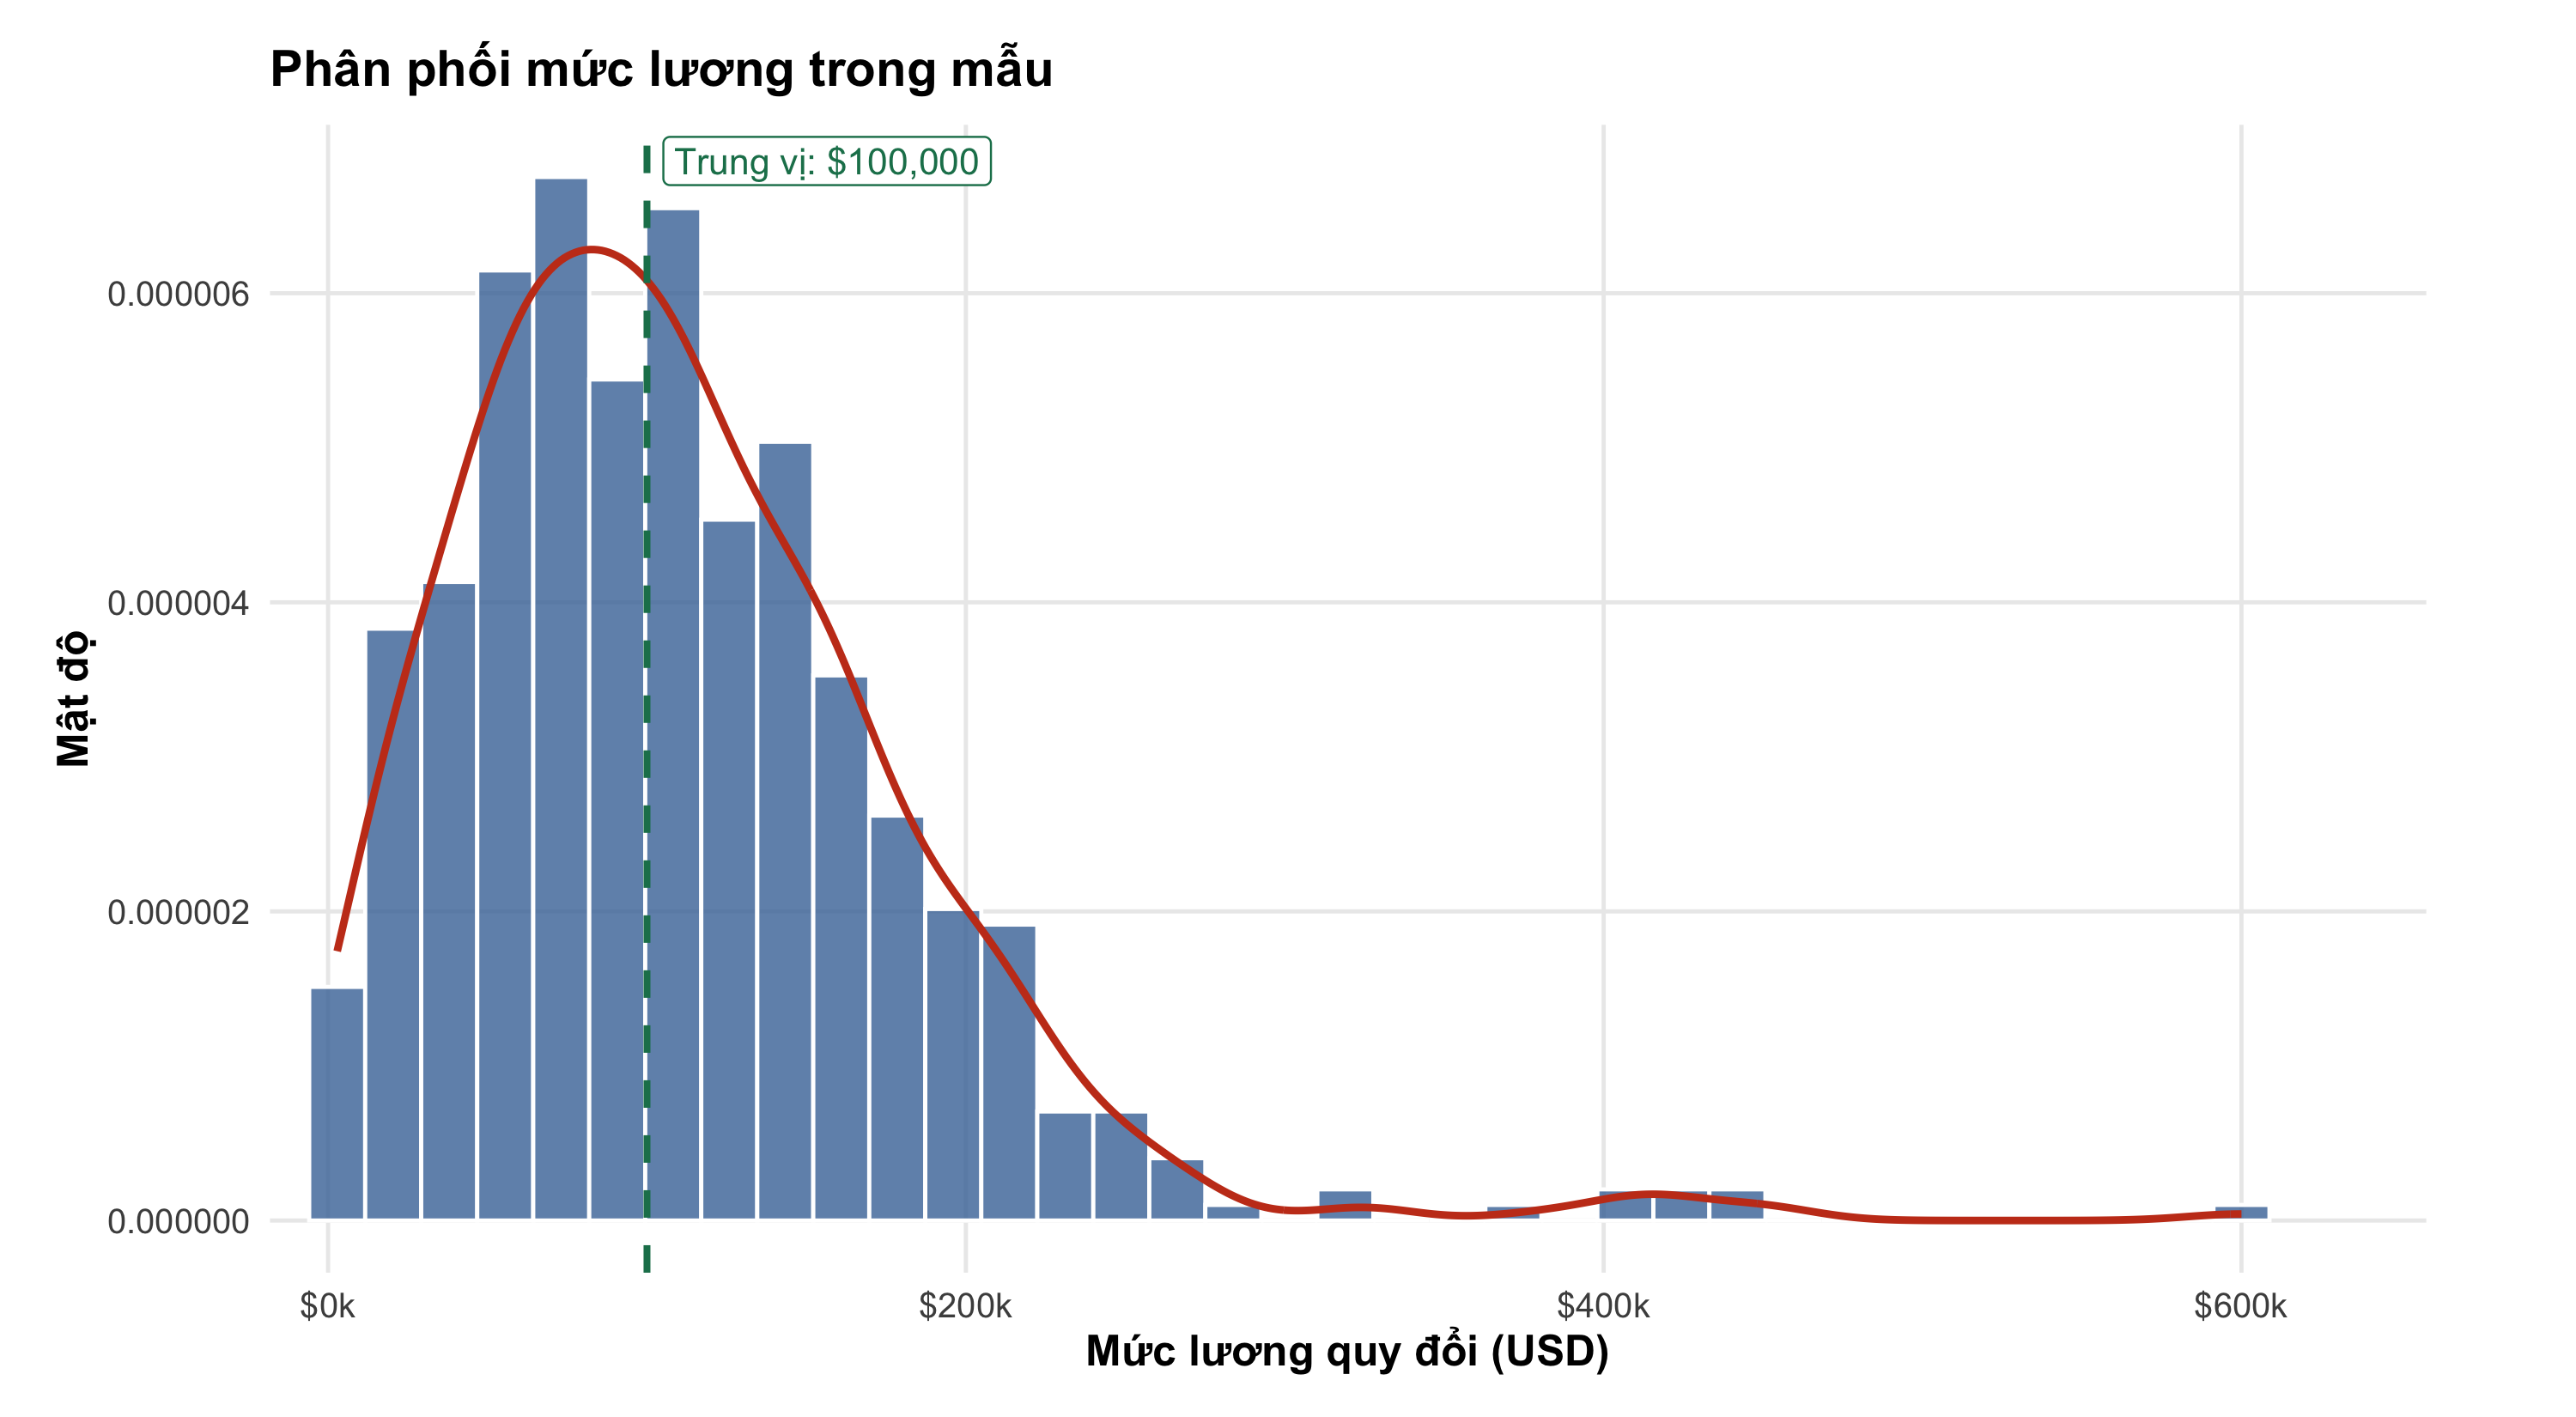
\includegraphics[width=1\linewidth]{img/nghi-salary-histogram-1.png} 

}

\caption{Phân phối mức lương quy đổi sang USD; đường đứt nét biểu diễn trung vị.}\label{nghi:fig:salary-histogram}
\end{figure}

Trung bình (\$110,610) cao hơn trung vị (\$100,000) khoảng \$10,600; độ
lệch (skewness) bằng 1,73 và mức lớn nhất \$600,000 xác nhận đuôi phải
kéo dài. Tuy nhiên, 50\% quan sát trung tâm đã trải từ \$60,757 đến
\$150,000, với IQR \$89,243, nên độ phân tán lớn không chỉ do một vài
mức lương cao. Trung vị và IQR vì vậy phản ánh vị trí và độ rộng của
phần trung tâm tốt hơn trung bình và độ lệch chuẩn trong các so sánh
nhóm. \texttt{salary\_in\_usd} có phân phối lệch phải và chứa một số mức
lương cao nhưng hợp lý về mặt nội dung. Đặc điểm này được lưu ý khi xây
dựng và đánh giá mô hình, nhưng không tự động dẫn đến việc biến đổi log.

\subsubsection{Mức lương theo các đặc điểm công
việc}\label{nghi:mux1ee9c-lux1b0ux1a1ng-theo-cuxe1c-ux111ux1eb7c-ux111iux1ec3m-cuxf4ng-viux1ec7c}

\begin{landscape}
\small
\begin{longtable}[]{@{}
  >{\raggedright\arraybackslash}p{(\linewidth - 12\tabcolsep) * \real{0.1780}}
  >{\raggedright\arraybackslash}p{(\linewidth - 12\tabcolsep) * \real{0.3305}}
  >{\raggedleft\arraybackslash}p{(\linewidth - 12\tabcolsep) * \real{0.0339}}
  >{\raggedleft\arraybackslash}p{(\linewidth - 12\tabcolsep) * \real{0.0932}}
  >{\raggedleft\arraybackslash}p{(\linewidth - 12\tabcolsep) * \real{0.1186}}
  >{\raggedleft\arraybackslash}p{(\linewidth - 12\tabcolsep) * \real{0.0763}}
  >{\raggedleft\arraybackslash}p{(\linewidth - 12\tabcolsep) * \real{0.1695}}@{}}
\caption{Thống kê mô tả mức lương theo các nhóm chính}\tabularnewline
\toprule\noalign{}
\begin{minipage}[b]{\linewidth}\raggedright
Đặc điểm
\end{minipage} & \begin{minipage}[b]{\linewidth}\raggedright
Nhóm
\end{minipage} & \begin{minipage}[b]{\linewidth}\raggedleft
n
\end{minipage} & \begin{minipage}[b]{\linewidth}\raggedleft
Trung bình
\end{minipage} & \begin{minipage}[b]{\linewidth}\raggedleft
Độ lệch chuẩn
\end{minipage} & \begin{minipage}[b]{\linewidth}\raggedleft
Trung vị
\end{minipage} & \begin{minipage}[b]{\linewidth}\raggedleft
Q1--Q3
\end{minipage} \\
\midrule\noalign{}
\endfirsthead
\toprule\noalign{}
\begin{minipage}[b]{\linewidth}\raggedright
Đặc điểm
\end{minipage} & \begin{minipage}[b]{\linewidth}\raggedright
Nhóm
\end{minipage} & \begin{minipage}[b]{\linewidth}\raggedleft
n
\end{minipage} & \begin{minipage}[b]{\linewidth}\raggedleft
Trung bình
\end{minipage} & \begin{minipage}[b]{\linewidth}\raggedleft
Độ lệch chuẩn
\end{minipage} & \begin{minipage}[b]{\linewidth}\raggedleft
Trung vị
\end{minipage} & \begin{minipage}[b]{\linewidth}\raggedleft
Q1--Q3
\end{minipage} \\
\midrule\noalign{}
\endhead
\bottomrule\noalign{}
\endlastfoot
Lĩnh vực nghề nghiệp & Data Science \& Research & 195 & \$115,791 &
\$74,561 & \$104,702 & \$62,058 -- \$153,084 \\
Lĩnh vực nghề nghiệp & Data Engineering \& Architecture & 168 &
\$117,668 & \$71,451 & \$109,512 & \$69,342 -- \$160,000 \\
Lĩnh vực nghề nghiệp & Data Analytics \& Business Intelligence & 118 &
\$99,393 & \$64,026 & \$93,350 & \$60,325 -- \$126,500 \\
Lĩnh vực nghề nghiệp & Machine Learning \& AI & 84 & \$100,226 &
\$77,490 & \$80,020 & \$45,046 -- \$128,250 \\
Kinh nghiệm & Entry-level / Junior & 88 & \$61,643 & \$44,396 & \$56,500
& \$27,505 -- \$85,426 \\
Kinh nghiệm & Mid-level / Intermediate & 208 & \$87,793 & \$64,119 &
\$76,940 & \$47,164 -- \$112,075 \\
Kinh nghiệm & Senior-level / Expert & 243 & \$138,375 & \$59,956 &
\$135,000 & \$99,532 -- \$171,881 \\
Kinh nghiệm & Executive-level / Director & 26 & \$199,392 & \$117,071 &
\$171,438 & \$130,006 -- \$233,750 \\
Nhóm tuyển dụng & Full-time & 546 & \$111,812 & \$70,791 & \$100,000 &
\$62,726 -- \$150,000 \\
Nhóm tuyển dụng & Other employment arrangements & 19 & \$76,083 &
\$103,282 & \$31,875 & \$13,983 -- \$100,000 \\
Quy mô công ty & Small & 82 & \$77,872 & \$63,815 & \$65,511 & \$41,816
-- \$100,000 \\
Quy mô công ty & Medium & 290 & \$114,807 & \$60,779 & \$109,640 &
\$70,822 -- \$150,214 \\
Quy mô công ty & Large & 193 & \$118,214 & \$86,753 & \$100,000 &
\$60,000 -- \$153,667 \\
Hình thức làm việc & On-site (0\%) & 121 & \$105,785 & \$68,393 &
\$98,158 & \$62,000 -- \$136,000 \\
Hình thức làm việc & Hybrid (50\%) & 98 & \$80,722 & \$57,639 & \$68,010
& \$50,000 -- \$99,926 \\
Hình thức làm việc & Fully remote (100\%) & 346 & \$120,763 & \$74,930 &
\$110,712 & \$70,000 -- \$159,750 \\
Khu vực cư trú & North America & 322 & \$145,659 & \$70,375 & \$135,000
& \$100,000 -- \$174,000 \\
Khu vực cư trú & Europe & 160 & \$69,200 & \$34,793 & \$63,278 &
\$46,422 -- \$87,932 \\
Khu vực cư trú & Asia & 60 & \$52,156 & \$54,233 & \$32,712 & \$17,766
-- \$66,083 \\
Khu vực cư trú & Others & 23 & \$60,493 & \$51,391 & \$40,038 & \$19,454
-- \$93,712 \\
Năm & 2020 & 72 & \$95,813 & \$82,832 & \$75,544 & \$45,724 --
\$115,526 \\
Năm & 2021 & 215 & \$99,430 & \$80,304 & \$82,528 & \$50,000 --
\$135,000 \\
Năm & 2022 & 278 & \$123,089 & \$59,889 & \$120,000 & \$78,791 --
\$160,000 \\
\end{longtable}
\end{landscape}

Theo quy mô công ty, khoảng cách chính nằm giữa Small với hai nhóm còn
lại: trung vị của Small là \$65,511, so với \$109,640 ở Medium và
\$100,000 ở Large. Khoảng Q1--Q3 của Medium và Large chồng lấp rộng, còn
Q3 của Small chỉ đạt mức trung vị của Large, cho thấy phần trung tâm của
phân phối tại doanh nghiệp nhỏ nằm thấp hơn. Việc Medium không thấp hơn
Large gợi ý mối liên hệ có dạng ngưỡng giữa Small và Medium/Large hơn là
tăng tuyến tính theo quy mô. Do đó, \texttt{company\_size} phù hợp với
cách biểu diễn phân loại thay vì áp đặt một hệ số tuyến tính theo thứ tự
S--M--L.

Fully remote có trung vị \$110,712, cao hơn On-site khoảng \$12,600 và
Hybrid khoảng \$42,700, nhưng các khoảng Q1--Q3 vẫn chồng lấp rộng. Mẫu
hình này có thể phản ánh việc các vị trí Fully remote tập trung nhiều
hơn ở North America, cấp Senior hoặc những nghề có thị trường tuyển dụng
quốc tế, thay vì một chênh lệch đồng nhất theo hình thức làm việc.
\texttt{remote\_ratio} vì vậy được giữ dưới dạng biến phân loại và được
xem xét cùng khu vực cư trú.

Sau khi gộp, nhóm \texttt{Other\ employment\ arrangements} có trung vị
\$31,875 và khoảng Q1--Q3 từ \$13,983 đến \$100,000, so với trung vị
\$100,000 của Full-time. Nhóm này chỉ gồm 19 quan sát và kết hợp ba hình
thức tuyển dụng khác nhau, nên độ phân tán lớn và mức trung tâm có thể
thay đổi đáng kể theo từng trường hợp. \texttt{employment\_group} được
sử dụng như một chỉ báo tuyển dụng khái quát, không hàm ý phân loại tình
trạng lao động chính thức hay không chính thức.

\begin{figure}

{\centering 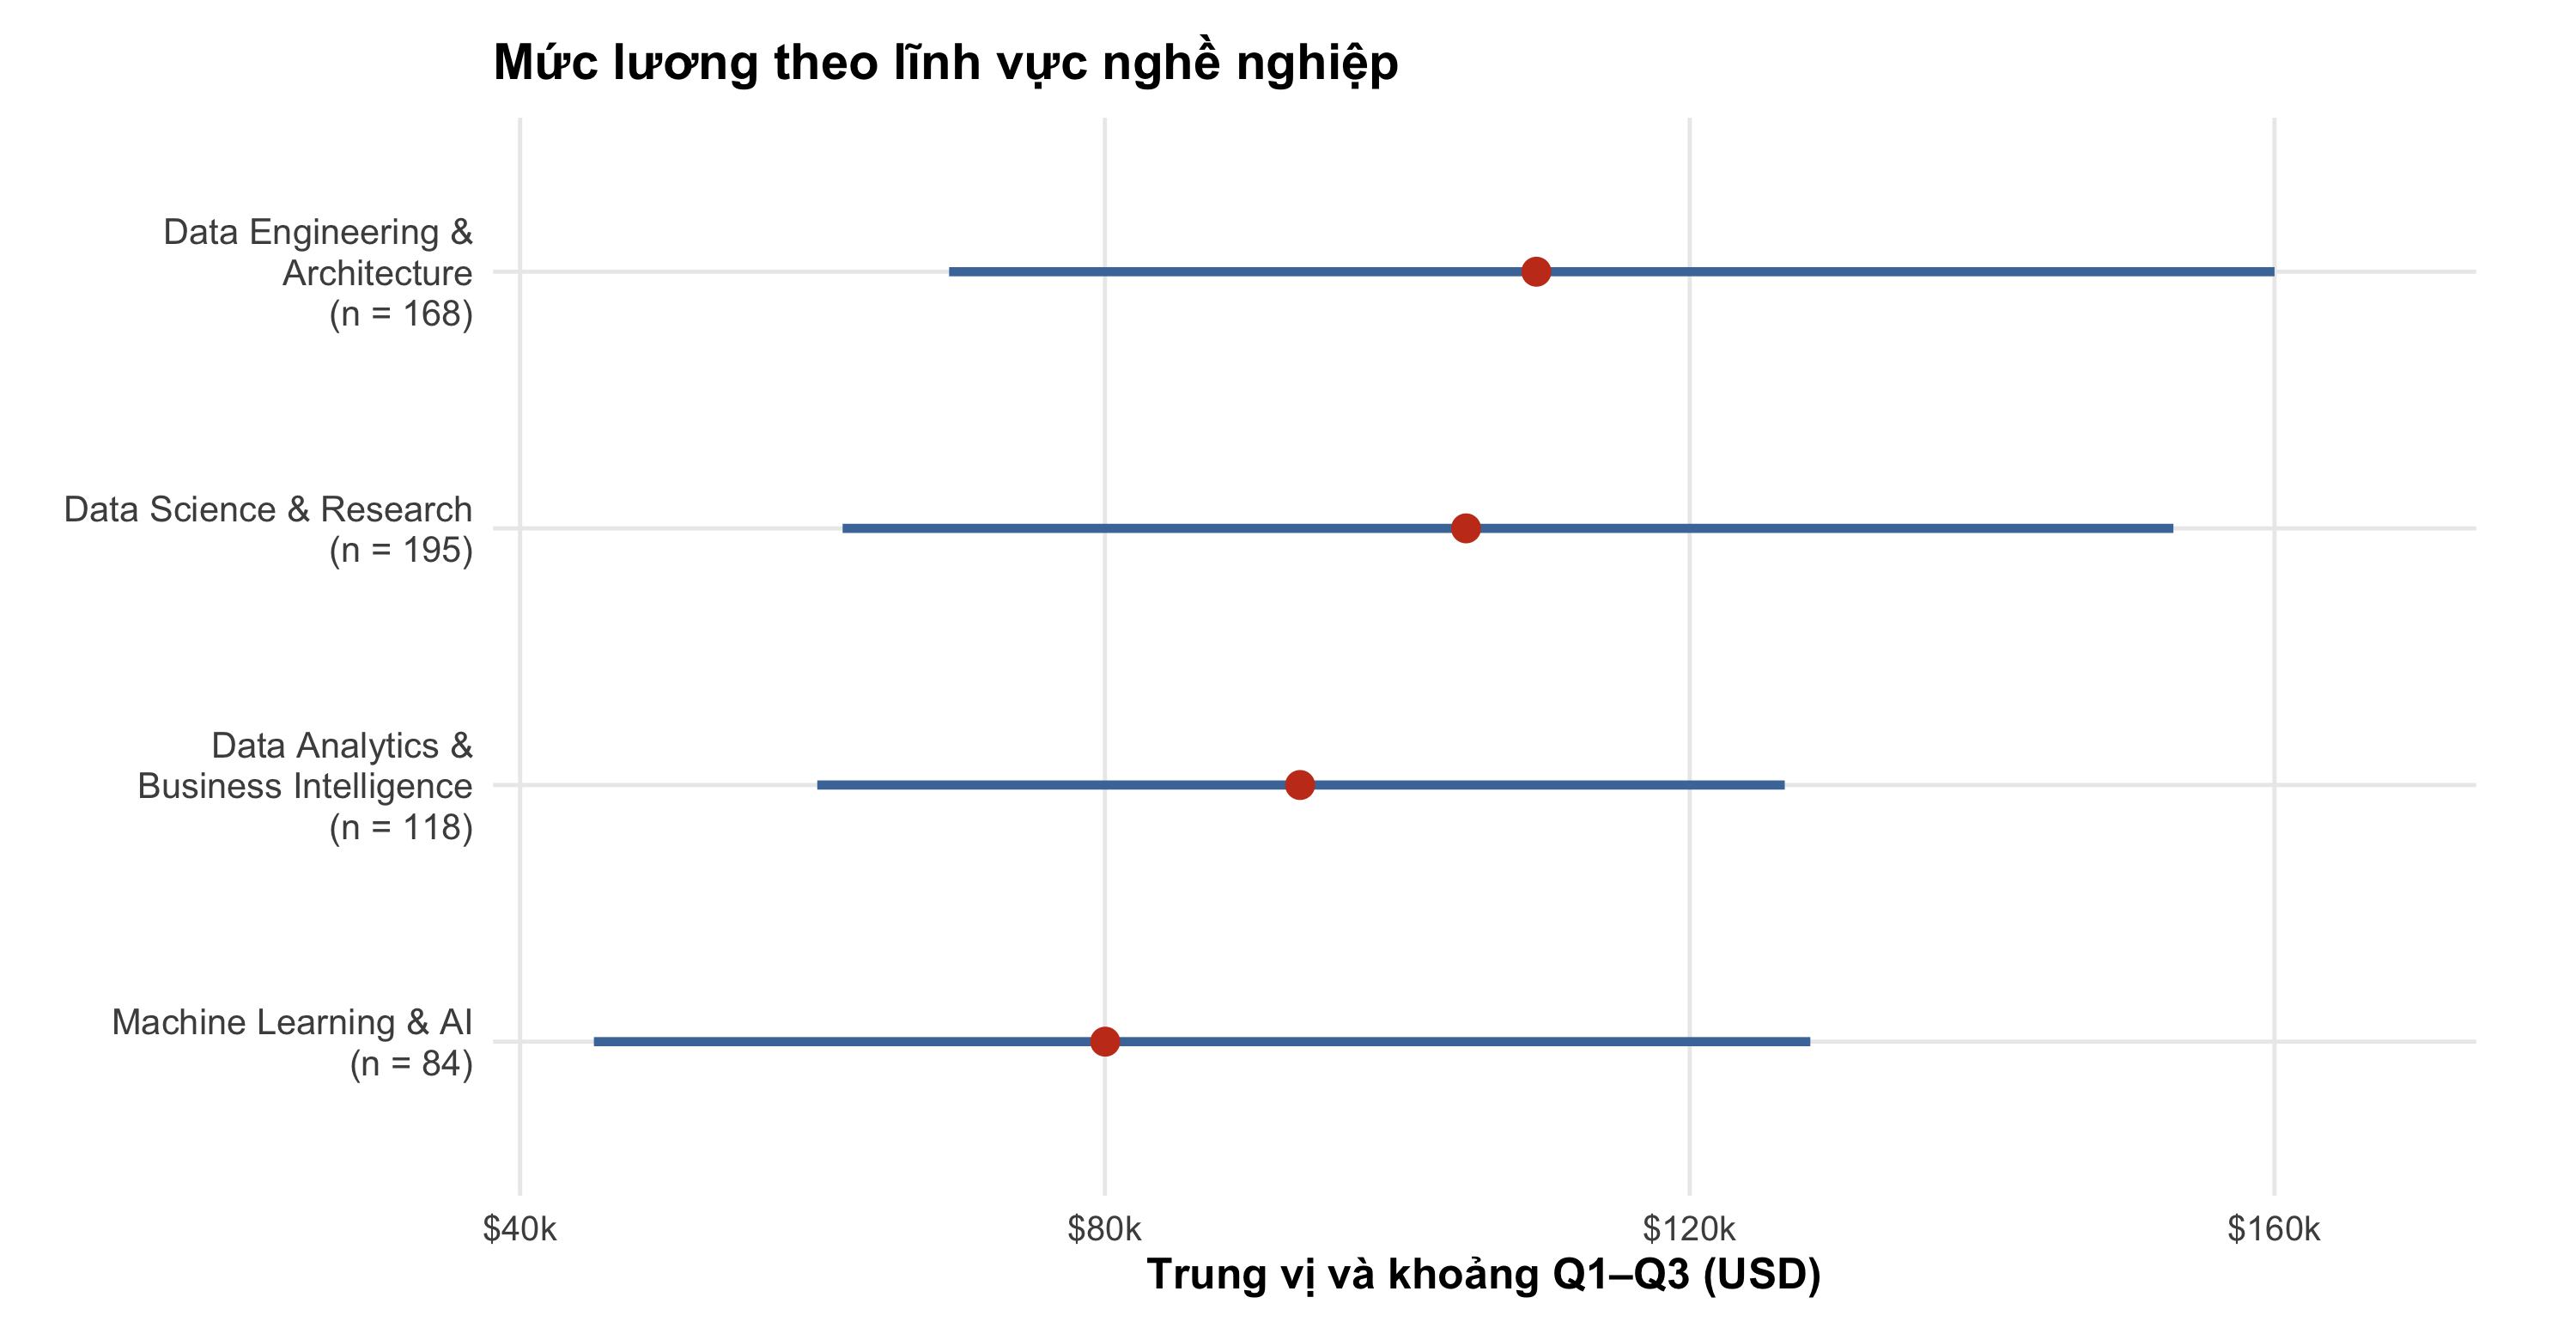
\includegraphics[width=1\linewidth]{img/nghi-plot-job-field-1.png} 

}

\caption{Trung vị và khoảng Q1–Q3 của mức lương theo lĩnh vực nghề nghiệp.}\label{nghi:fig:plot-job-field}
\end{figure}

Trung vị giữa bốn lĩnh vực trải từ \$80,020 ở Machine Learning \& AI đến
\$109,512 ở Data Engineering \& Architecture, tức chênh lệch khoảng
\$29,500. Tuy vậy, các khoảng Q1--Q3 chồng lấp rộng, nên phần trung tâm
của bốn phân phối chưa tách biệt rõ như thứ hạng trung vị gợi ý. Riêng
Machine Learning \& AI có trung bình cao hơn trung vị khoảng \$20,200 và
độ phân tán lớn, cho thấy một số mức lương cao kéo trung bình lên trong
khi phần giữa của phân phối vẫn thấp hơn. Chênh lệch theo lĩnh vực có
thể phản ánh nhiệm vụ chuyên môn và nhu cầu thị trường, nhưng cũng phụ
thuộc vào cơ cấu kinh nghiệm, khu vực và năm; vì vậy kết quả theo
\texttt{job\_field} cần được xem xét đồng thời với các đặc điểm này thay
vì diễn giải riêng lẻ.

\begin{figure}

{\centering 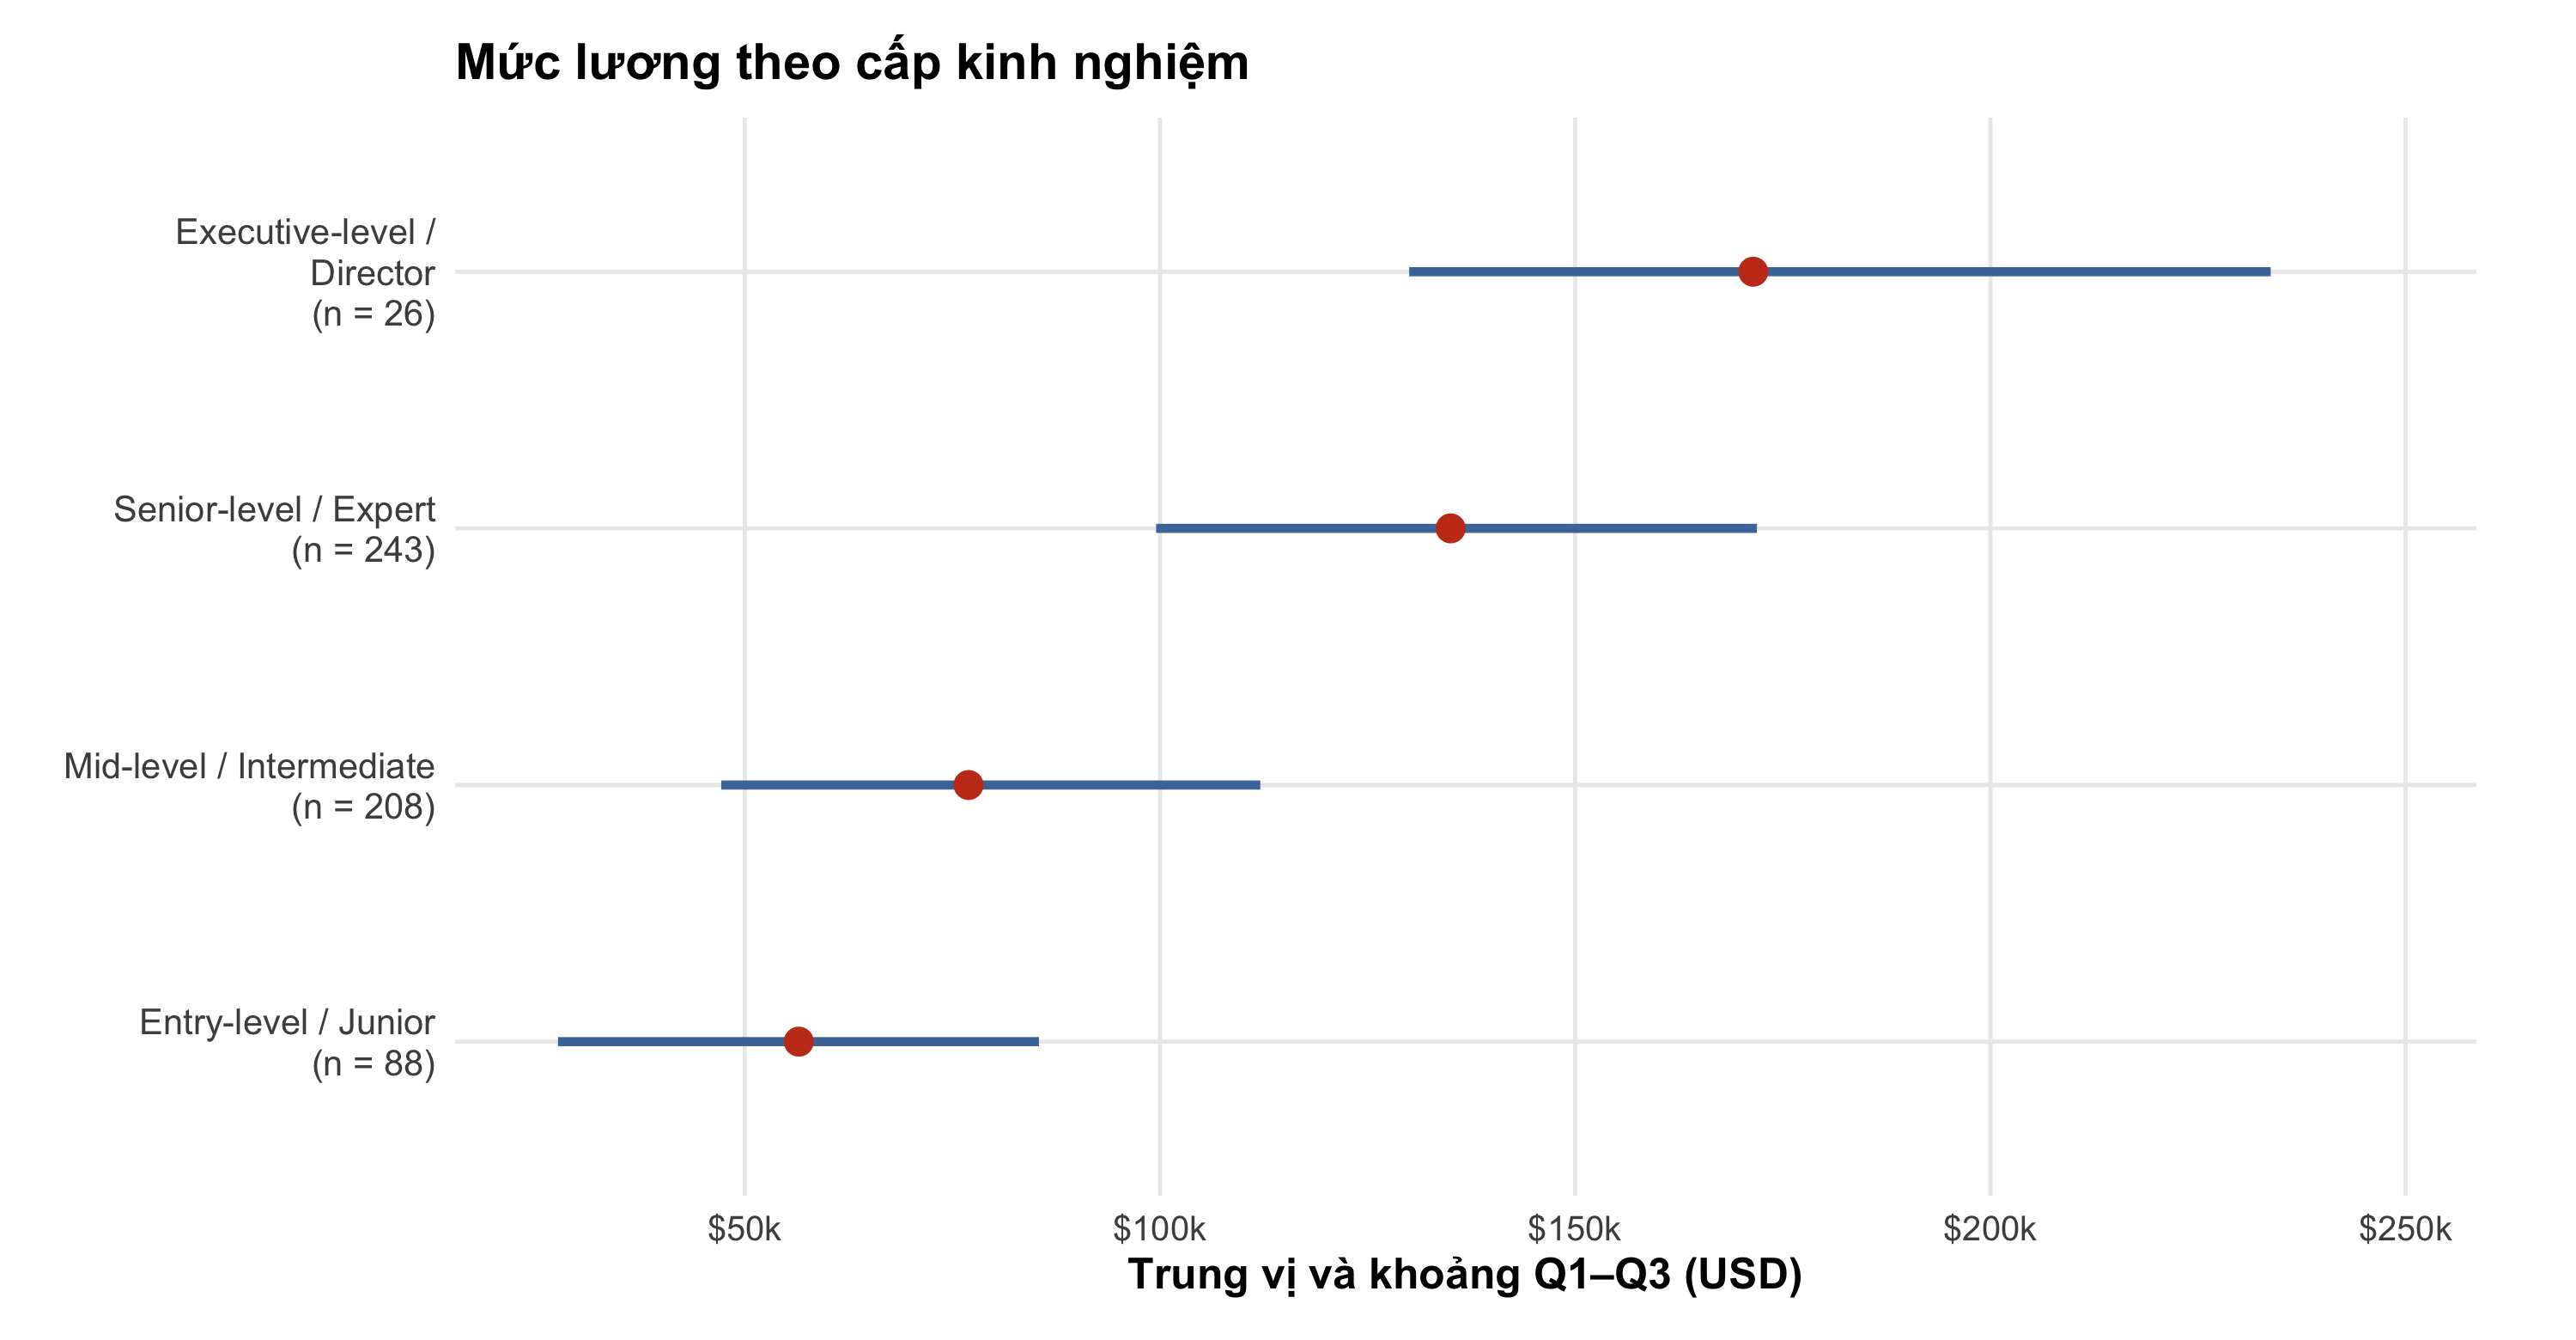
\includegraphics[width=1\linewidth]{img/nghi-plot-experience-1.png} 

}

\caption{Trung vị và khoảng Q1–Q3 của mức lương theo cấp kinh nghiệm.}\label{nghi:fig:plot-experience}
\end{figure}

Trung vị lương tăng liên tục từ \$56,500 ở Entry-level lên \$76,940 ở
Mid-level, \$135,000 ở Senior và \$171,438 ở Executive; bước tăng lớn
nhất, khoảng \$58,100, xuất hiện giữa Mid-level và Senior. Q3 của
Entry-level (\$85,426) vẫn thấp hơn Q1 của Senior (\$99,532), cho thấy
sự phân tầng lương giữa hai cấp này phản ánh dịch chuyển của phần trung
tâm chứ không chỉ một vài mức lương cao. Khoảng Q1--Q3 của Executive
rộng từ \$130,006 đến \$233,750 và nhóm chỉ có 26 quan sát, nên mức
lương ở cấp cao nhất biến động lớn hơn và ước lượng trung tâm kém ổn
định hơn. Mẫu hình tăng có thứ tự nhưng khoảng cách không đều cho thấy
kinh nghiệm có liên hệ rõ với mức lương, đồng thời độ lớn chênh lệch cần
được đặt trong cơ cấu nghề nghiệp của từng cấp.

\begin{figure}

{\centering 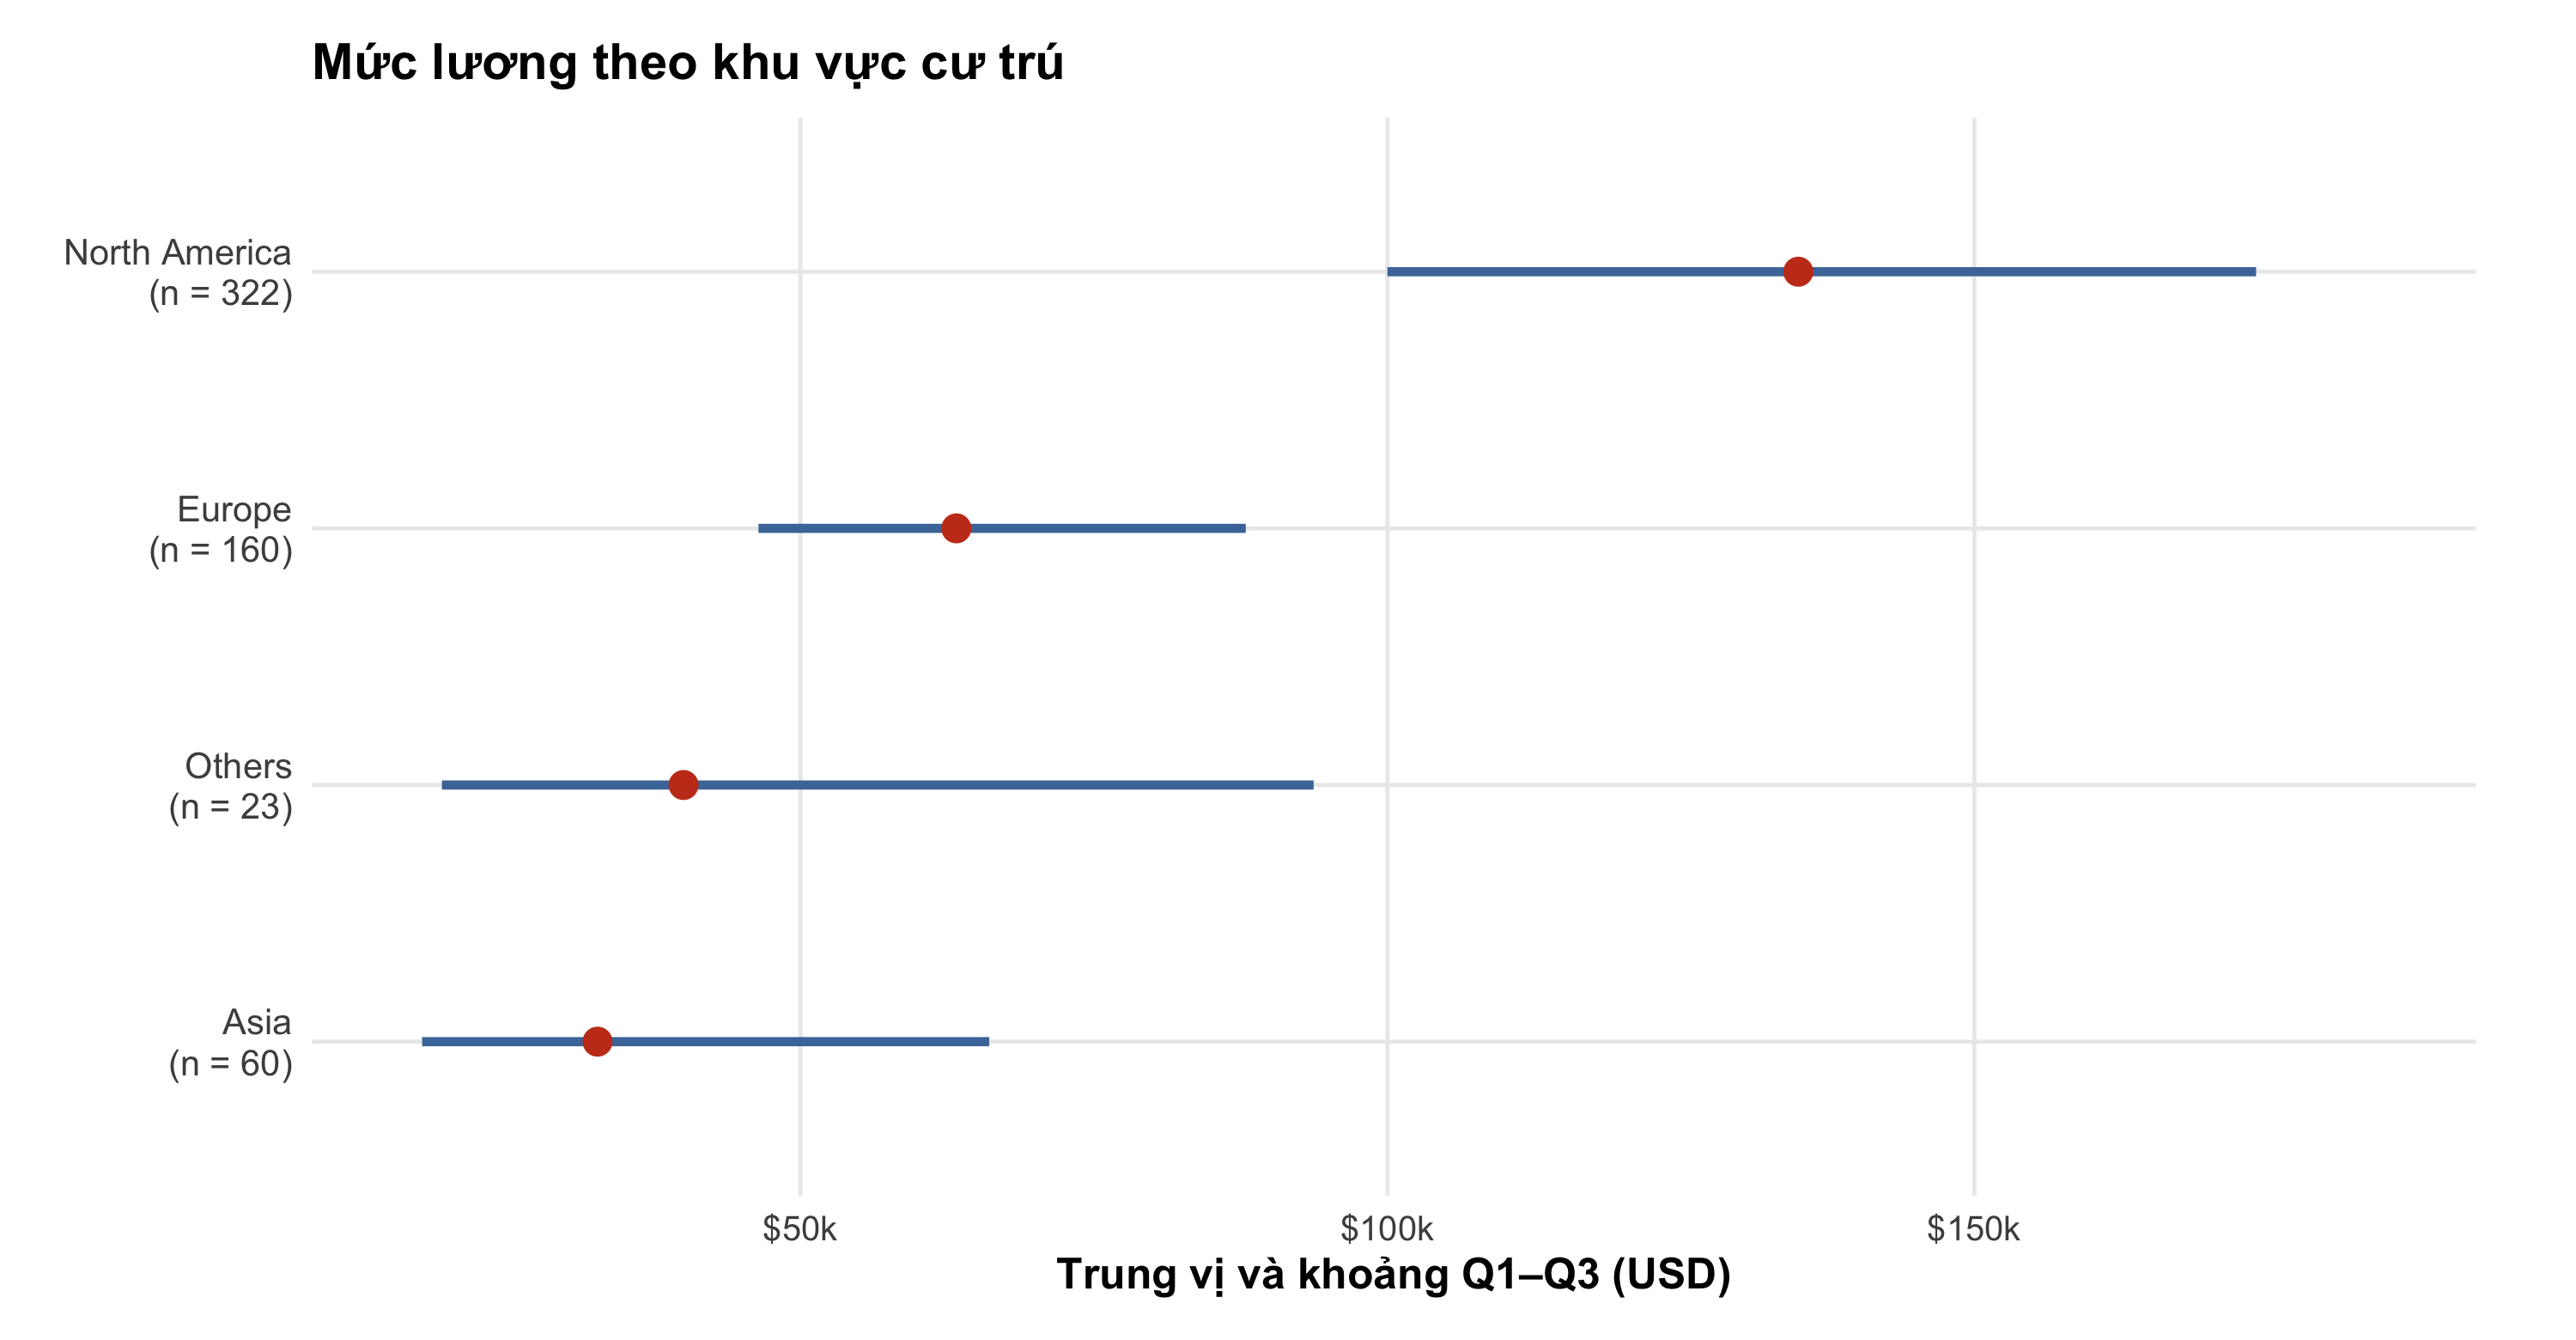
\includegraphics[width=1\linewidth]{img/nghi-plot-region-1.png} 

}

\caption{Trung vị và khoảng Q1–Q3 của mức lương theo khu vực cư trú.}\label{nghi:fig:plot-region}
\end{figure}

North America có trung vị \$135,000, cao hơn Europe khoảng \$71,700 và
gấp hơn bốn lần trung vị của Asia. Q1 của North America (\$100,000) còn
vượt Q3 của Europe (\$87,932), cho thấy phần trung tâm của hai phân phối
gần như tách biệt; giữa Europe và Asia, chênh lệch trung vị khoảng
\$30,600 nhưng hai khoảng Q1--Q3 vẫn chồng lấp. Khoảng cách này có thể
phản ánh mặt bằng lương, cấu trúc thị trường lao động, cơ cấu nghề
nghiệp và kinh nghiệm khác nhau giữa các khu vực, đồng thời mức lương
USD chưa được điều chỉnh theo sức mua. Khu vực cư trú vì vậy có khả năng
đóng góp đáng kể vào dự báo và cần được giữ trong mô hình cùng các biến
nghề nghiệp; \texttt{Others} chỉ là nhóm tổng hợp của ba khu vực thưa,
không đại diện cho một thị trường lao động đồng nhất.

\subsubsection{Phân tích kết
hợp}\label{nghi:phuxe2n-tuxedch-kux1ebft-hux1ee3p}

Phân tích kết hợp xem xét lĩnh vực nghề nghiệp theo cấp kinh nghiệm và
khu vực cư trú theo hình thức làm việc. Hai biểu đồ cho phép đánh giá
liệu chênh lệch quan sát được giữa các nhóm có duy trì giống nhau khi
xét thêm đặc điểm đi kèm hay không.

\begin{figure}

{\centering 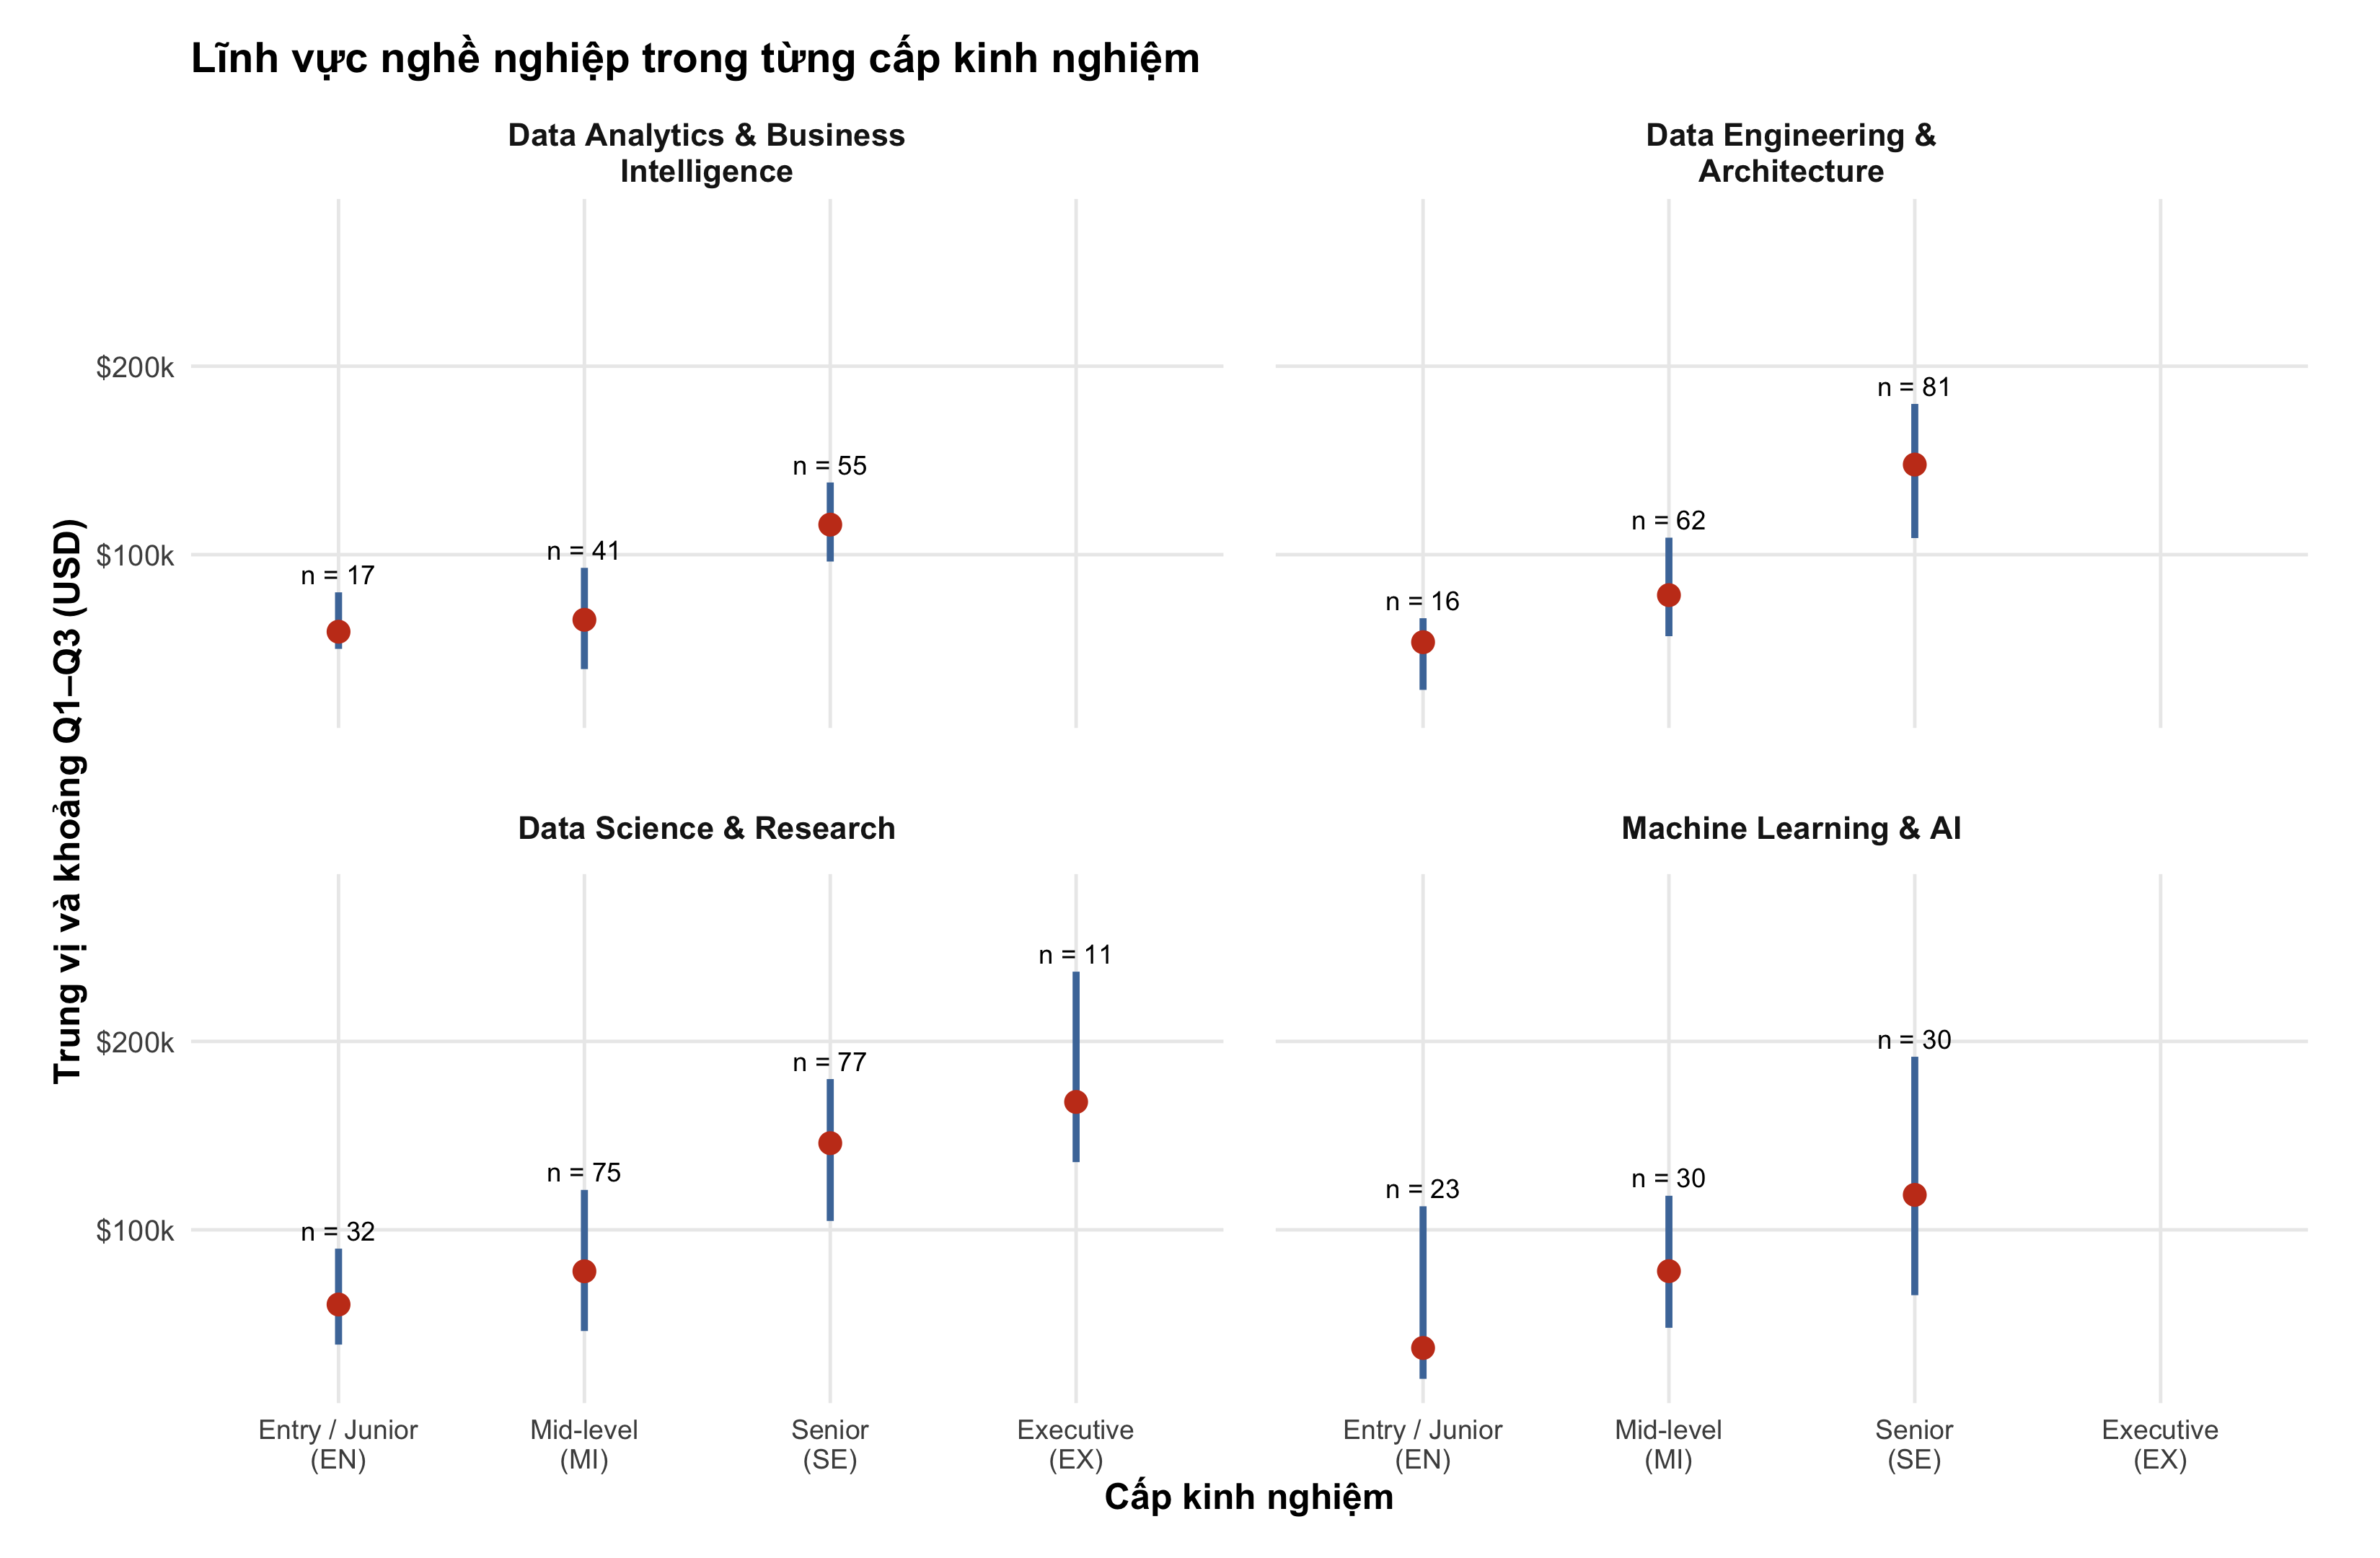
\includegraphics[width=1\linewidth]{img/nghi-interaction-field-experience-1.png} 

}

\caption{Trung vị và khoảng Q1–Q3 theo lĩnh vực nghề nghiệp và kinh nghiệm; chỉ gồm tổ hợp có n \(\geq\) 10.}\label{nghi:fig:interaction-field-experience}
\end{figure}

Ở Entry-level, Machine Learning \& AI có trung vị khoảng \$37,300, thấp
hơn ba lĩnh vực còn lại ở mức \$53,500--\$60,400; đến Mid-level, nhóm
này tăng lên khoảng \$78,100 và gần bằng Data Science \& Research cùng
Data Engineering \& Architecture. Tại Senior, hai lĩnh vực Data Science
và Data Engineering đạt khoảng \$146,000--\$147,800, cao hơn Data
Analytics và Machine Learning khoảng \$27,000--\$32,000, cho thấy khoảng
cách giữa các lĩnh vực mở rộng trở lại ở cấp kinh nghiệm cao. Các khoảng
Q1--Q3 vẫn chồng lấp, đặc biệt Machine Learning \& AI có độ phân tán
rộng; các quan sát Executive được phân tán giữa nhiều lĩnh vực nên cỡ
mẫu của từng tổ hợp nhỏ hơn các cấp còn lại và phản ánh xu hướng ban
đầu. Sự thay đổi cả thứ hạng lẫn độ lớn chênh lệch cho thấy mối liên hệ
giữa lĩnh vực nghề nghiệp và mức lương không hoàn toàn đồng nhất giữa
các cấp kinh nghiệm.

\begin{figure}

{\centering 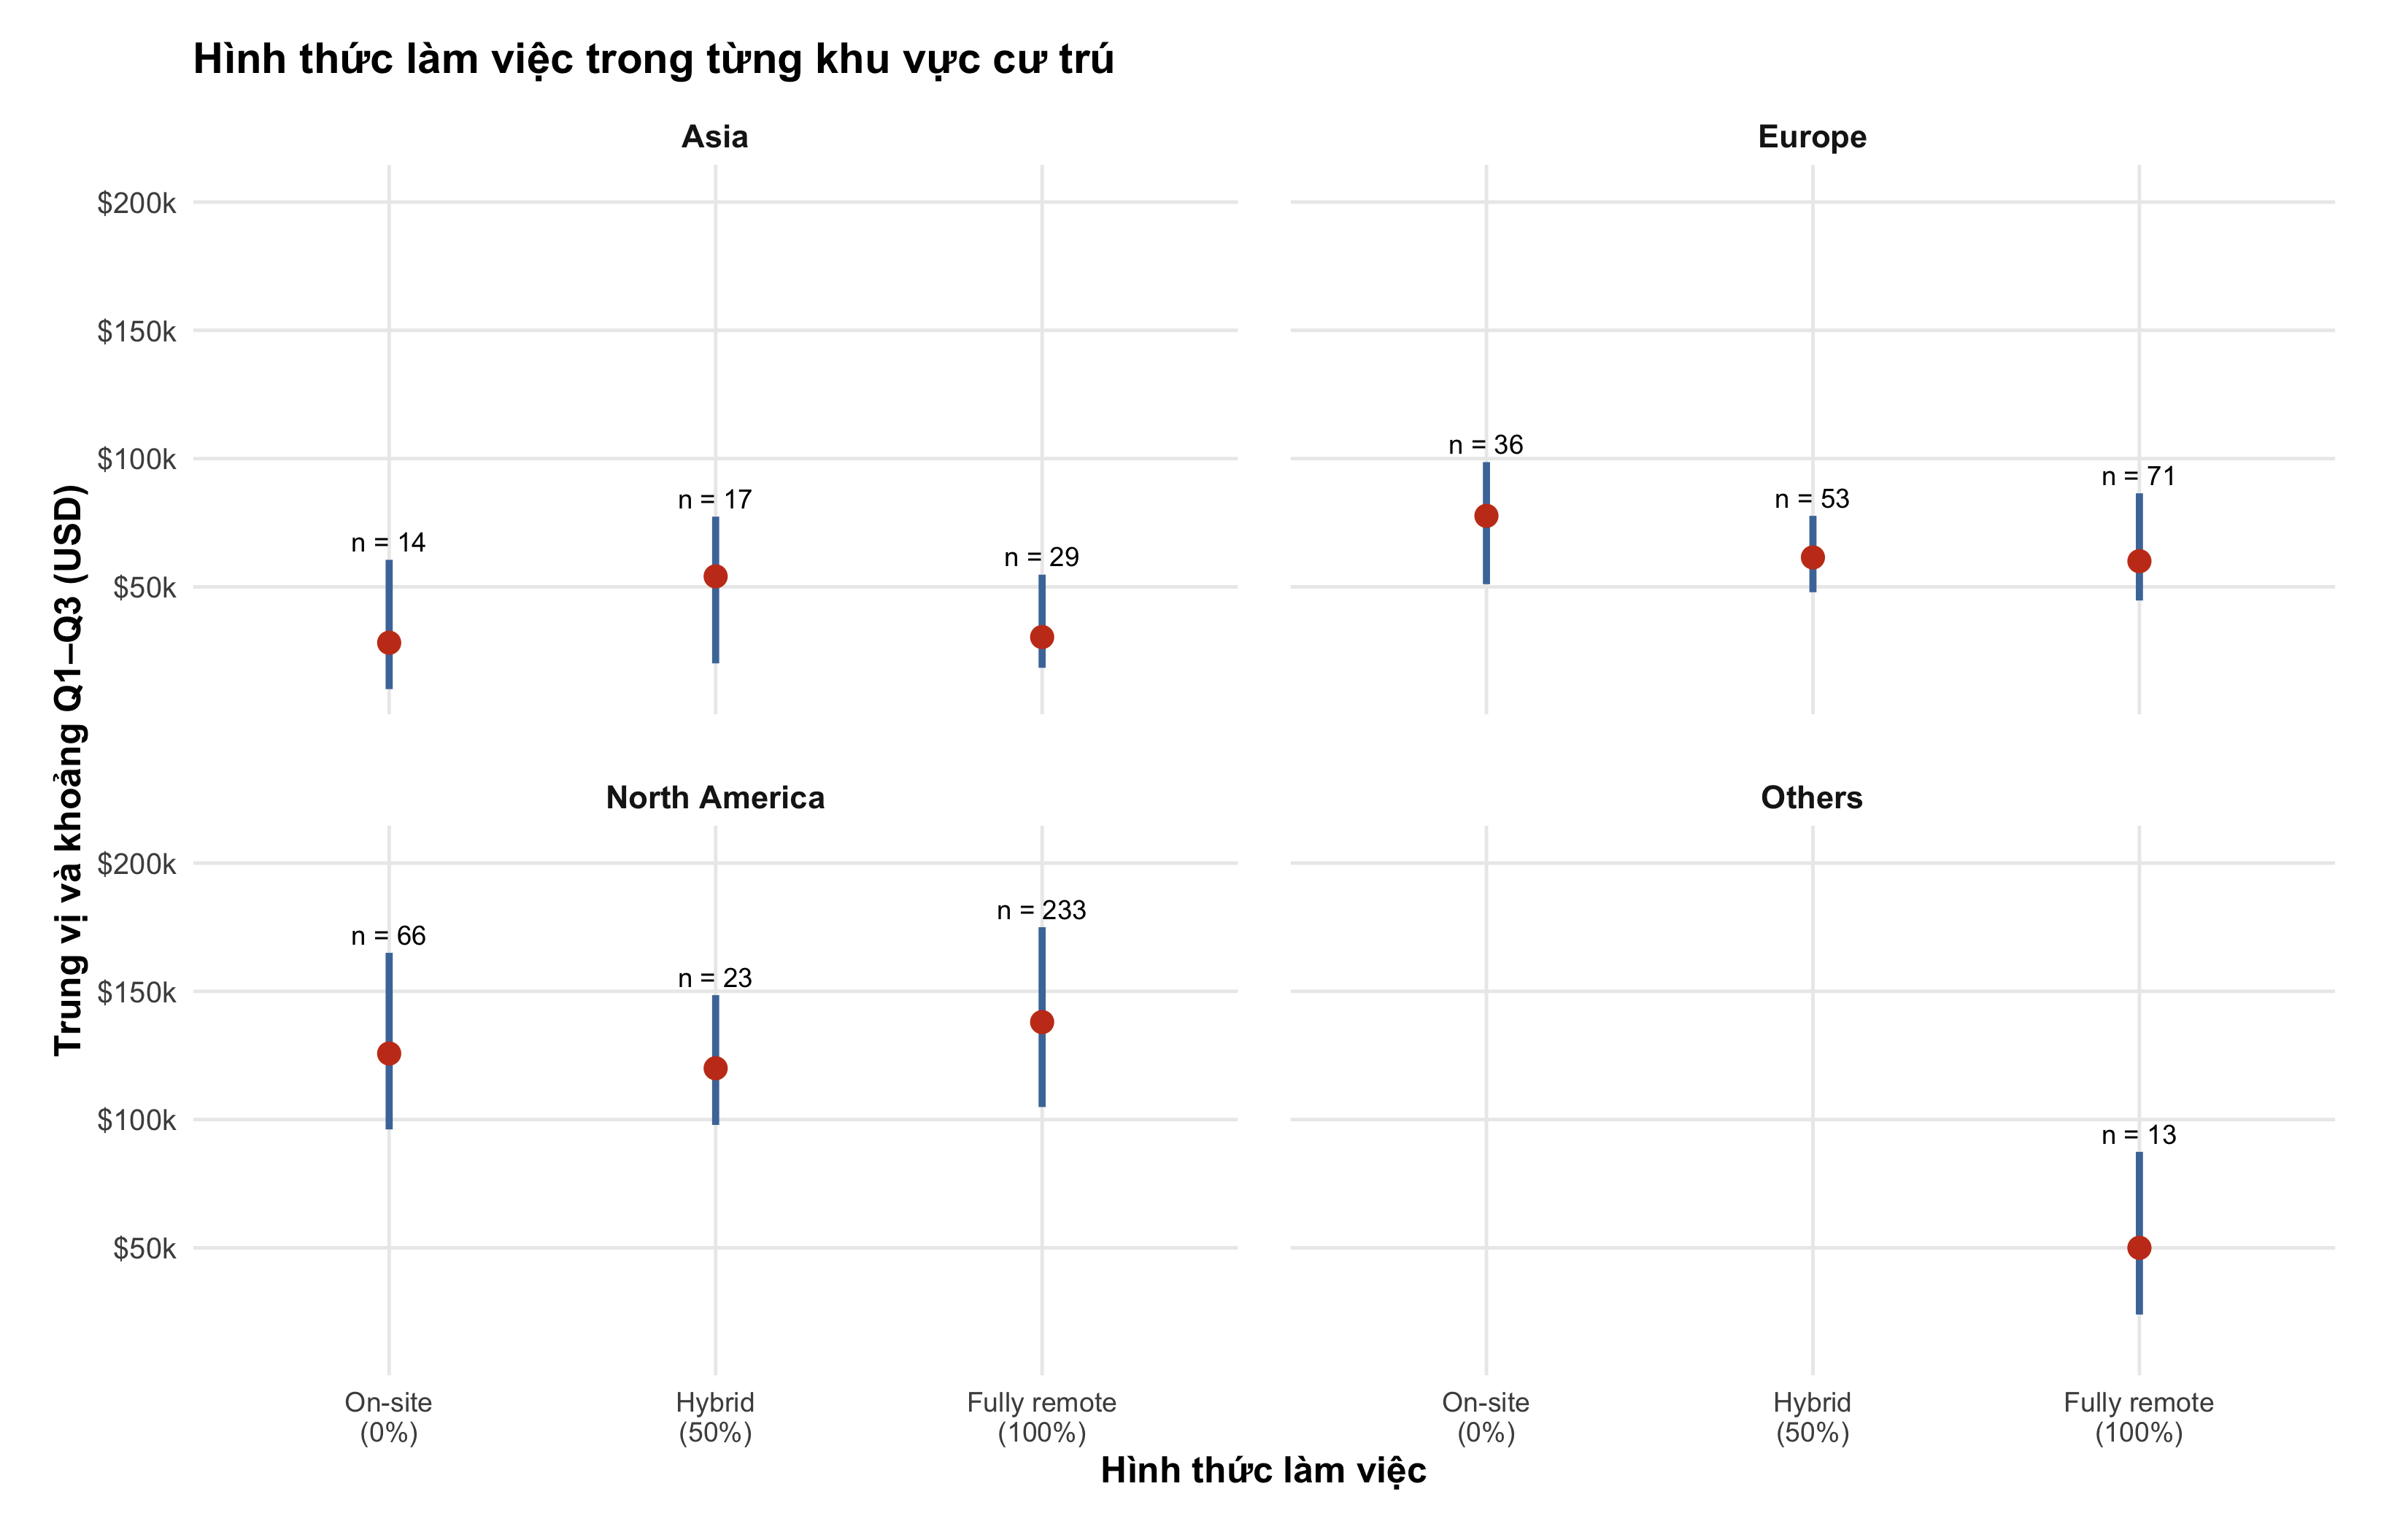
\includegraphics[width=1\linewidth]{img/nghi-interaction-region-remote-1.png} 

}

\caption{Trung vị và khoảng Q1–Q3 theo khu vực cư trú và hình thức làm việc; chỉ gồm tổ hợp có n \(\geq\) 10.}\label{nghi:fig:interaction-region-remote}
\end{figure}

Tại North America, Fully remote có trung vị \$138,000, cao hơn On-site
và Hybrid lần lượt khoảng \$12,300 và \$18,000; các khoảng Q1--Q3 vẫn
chồng lấp rộng nên mức chênh lệch trong khu vực này tương đối hạn chế.
Tại Europe, Fully remote có trung vị \$60,000, thấp hơn On-site khoảng
\$17,700, trong khi tại Asia nhóm Hybrid cao hơn cả On-site và Fully
remote khoảng \$24,000--\$26,000. Chiều của chênh lệch vì vậy thay đổi
giữa các khu vực, trái với ấn tượng từ thống kê chung rằng Fully remote
luôn gắn với mức lương cao hơn. Một số tổ hợp tại Asia và
\texttt{Others} có cỡ mẫu nhỏ hơn, nên kết quả chủ yếu cho thấy mối liên
hệ giữa hình thức làm việc và mức lương không đồng nhất giữa các khu
vực.

\subsubsection{Thay đổi mức lương theo thời
gian}\label{nghi:thay-ux111ux1ed5i-mux1ee9c-lux1b0ux1a1ng-theo-thux1eddi-gian}

\begin{figure}

{\centering 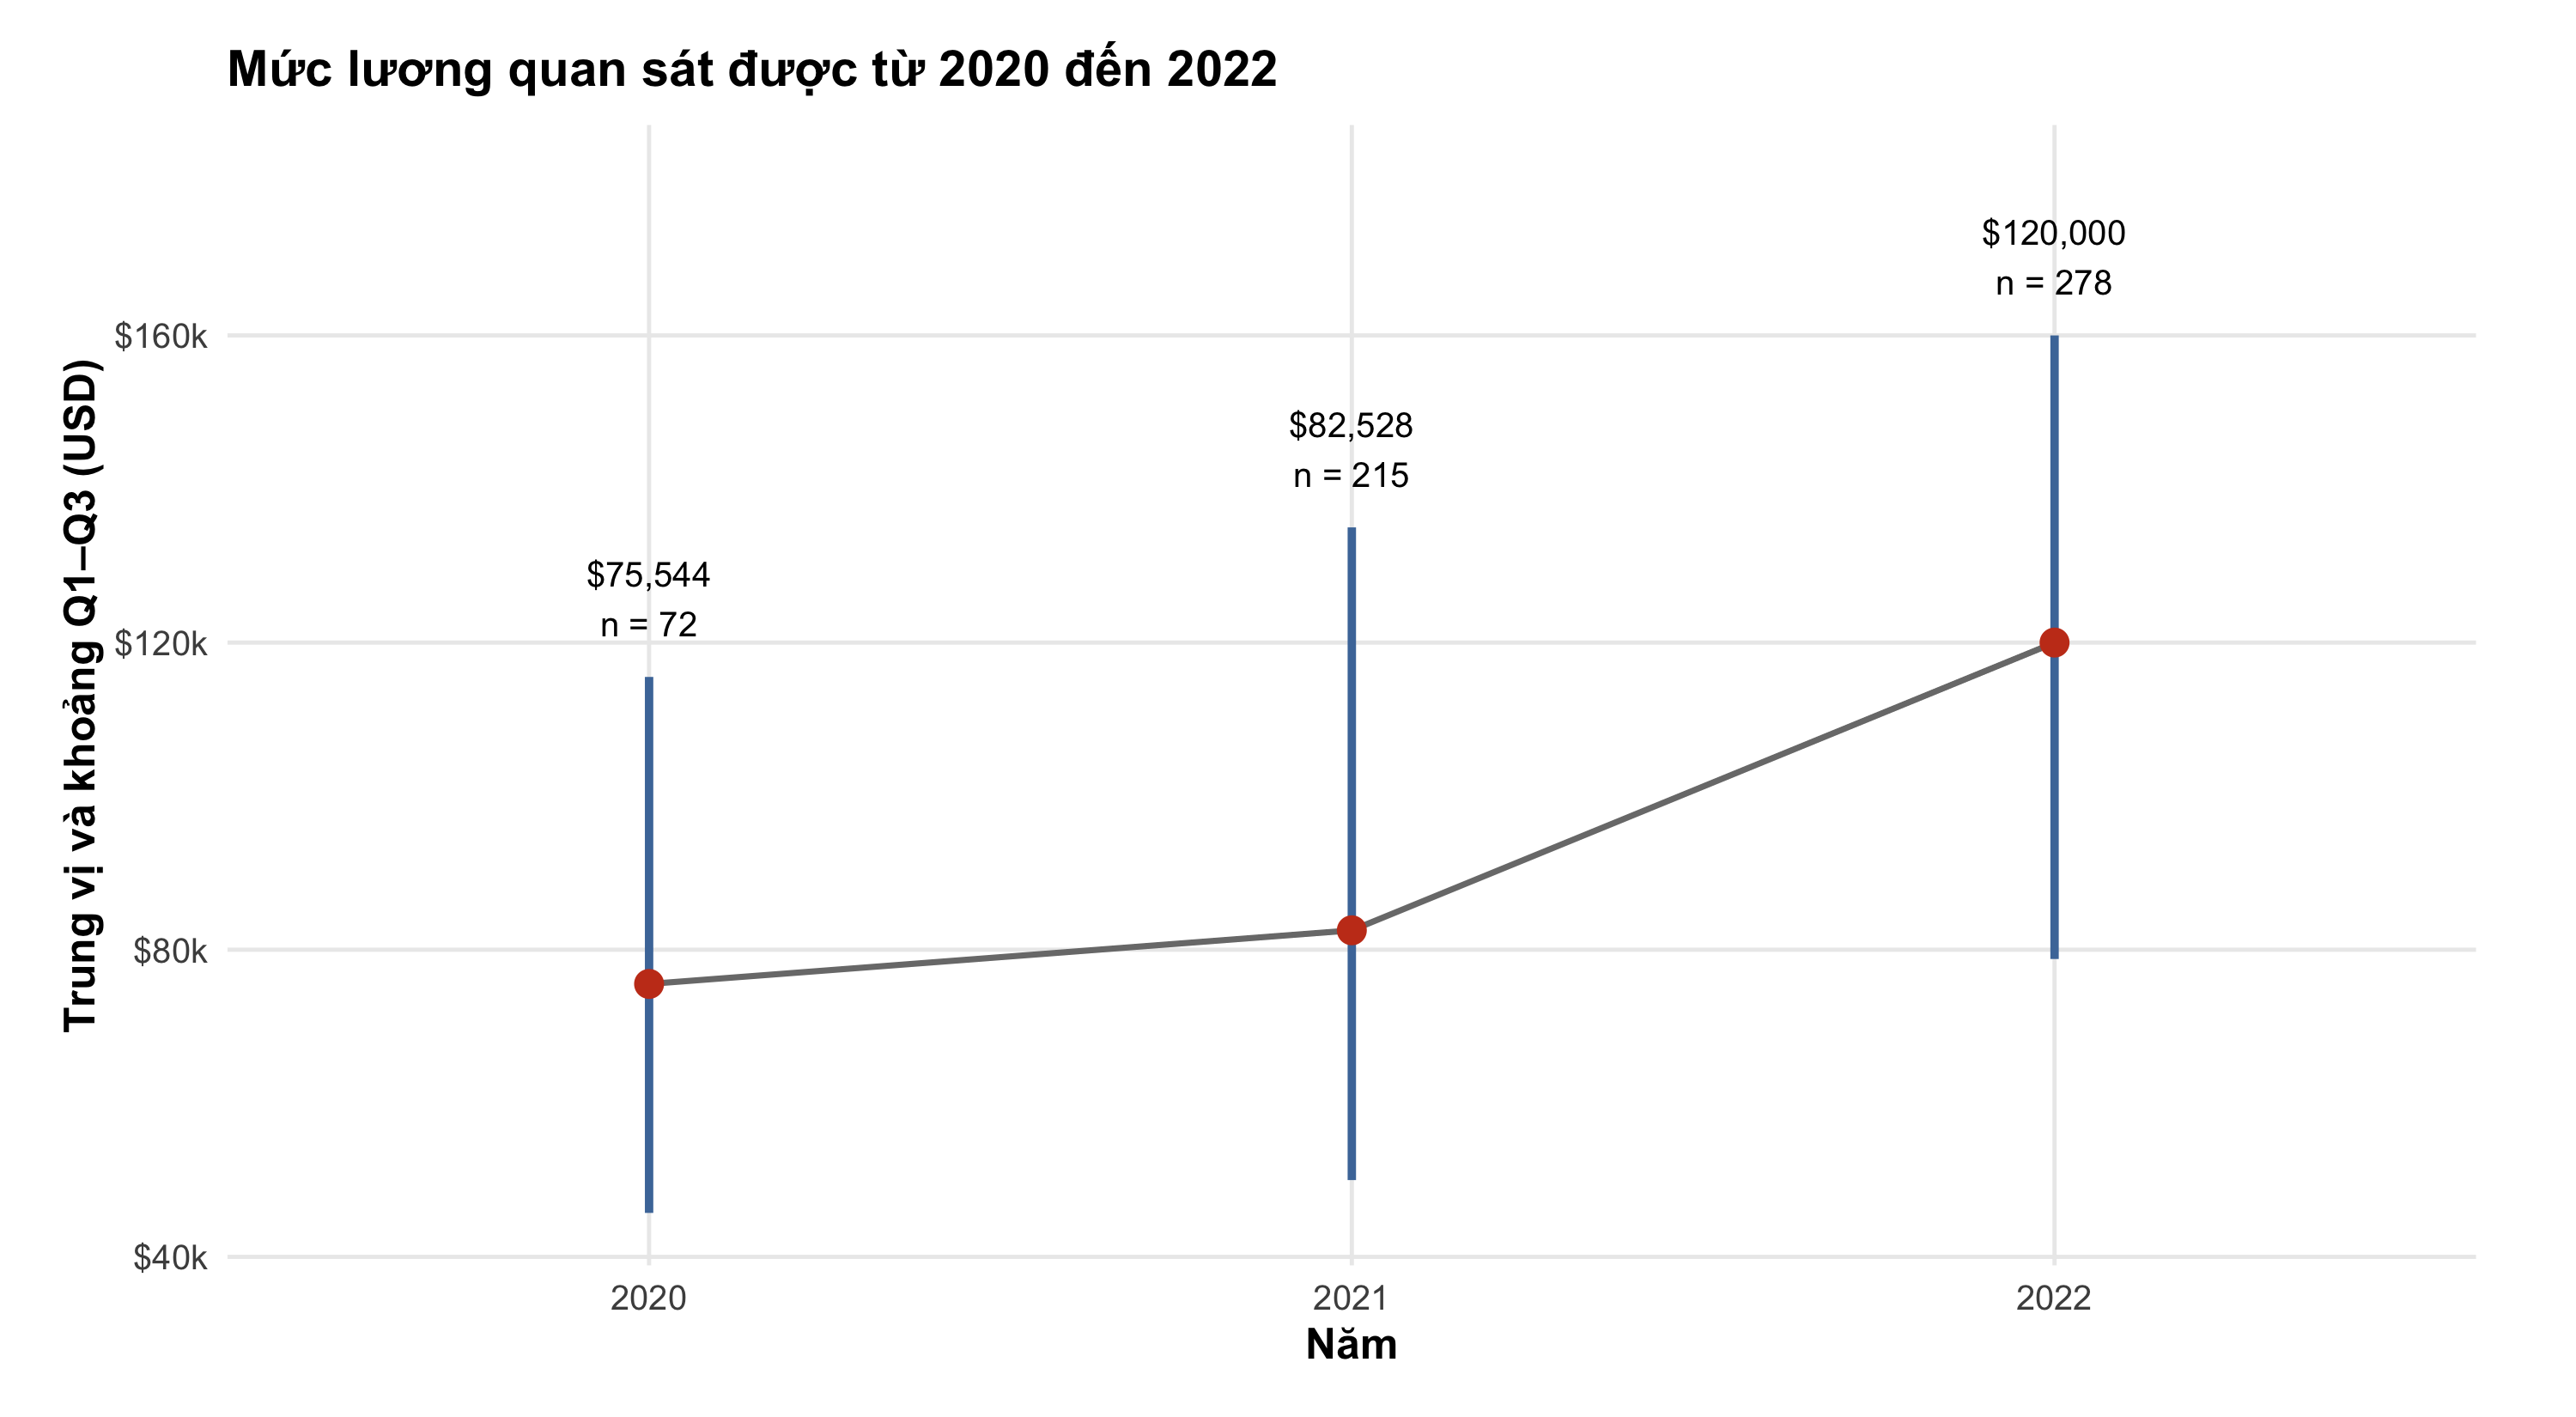
\includegraphics[width=1\linewidth]{img/nghi-year-plot-1.png} 

}

\caption{Trung vị và khoảng Q1–Q3 của mức lương theo năm quan sát.}\label{nghi:fig:year-plot}
\end{figure}

Từ 2020 đến 2021, trung vị chỉ tăng khoảng \$7,000 và trung bình tăng
khoảng \$3,600, trong khi hai khoảng Q1--Q3 chồng lấp rộng. Bước chuyển
sang 2022 rõ hơn: trung vị tăng khoảng \$37,500, trung bình tăng khoảng
\$23,700, đồng thời cả Q1 và Q3 đều dịch lên, gợi ý phần trung tâm của
phân phối tăng chứ không chỉ xuất hiện thêm một vài mức lương cao. Tuy
nhiên, năm 2022 chiếm gần một nửa mẫu và cơ cấu nghề nghiệp, kinh
nghiệm, khu vực hoặc quy mô công ty có thể khác hai năm trước. Mức tăng
không đều cho thấy ba năm nên được diễn giải như các thời kỳ rời rạc,
không phải một xu hướng tuyến tính dài hạn.

Sau tiền xử lý, dữ liệu còn 565 quan sát, không có giá trị khuyết hoặc
mã không hợp lệ; 42 dòng trùng hoàn toàn đã được loại. Phân phối lương
lệch phải, nhưng IQR rộng cho thấy mức độ không đồng nhất đáng kể ngay
trong 50\% quan sát trung tâm. Mười ngoại lai theo quy tắc 1,5 \(\times\) IQR
không có dấu hiệu rõ ràng của lỗi nhập liệu nên được giữ nguyên trong dữ
liệu.

Kinh nghiệm và khu vực cư trú tạo ra những dịch chuyển rõ nhất trong
phần trung tâm của phân phối, trong khi quy mô công ty biểu hiện hiệu
ứng ngưỡng giữa Small và Medium/Large. Chênh lệch theo lĩnh vực nghề
nghiệp vừa nhỏ hơn vừa phụ thuộc vào cấp kinh nghiệm; tương tự, thứ tự
lương giữa các hình thức làm việc đổi chiều theo khu vực. Bước tăng nổi
bật ở năm 2022 cũng cho thấy biến thời gian không nên được giả định có
quan hệ tuyến tính đơn giản với mức lương.

Các kết quả cho thấy kinh nghiệm, nghề nghiệp, quy mô công ty, hình thức
làm việc, khu vực và năm đều có liên hệ với mức lương ở những mức độ
khác nhau. Chênh lệch quan sát được giữa một số nhóm cũng thay đổi theo
đặc điểm đi kèm. Tuy nhiên, các kết quả này chưa kiểm soát đồng thời các
yếu tố và không cung cấp bằng chứng về quan hệ nhân quả. Vì vậy, các mô
hình được xây dựng để xét đồng thời các biến dự báo và đánh giá khả năng
dự báo ngoài mẫu.

\subsection{Mục tiêu nghiên
cứu}\label{nghi:mux1ee5c-tiuxeau-nghiuxean-cux1ee9u}

Trên cơ sở đặc điểm dữ liệu và các mẫu hình được nhận diện trong EDA,
nghiên cứu tập trung vào hai mục tiêu chính.

\textbf{Mục tiêu 1 -- Dự báo mức lương bằng các mô hình hồi quy.} Xây
dựng và so sánh OLS, Ridge Regression và LASSO Regression trong dự báo
mức lương, từ đó lựa chọn mô hình hồi quy có khả năng dự báo ngoài mẫu
phù hợp nhất.

\textbf{Mục tiêu 2 -- Đánh giá khả năng cải thiện dự báo bằng CatBoost.}
Xây dựng CatBoost như một hướng mở rộng và đánh giá liệu mô hình này có
cải thiện khả năng dự báo mức lương ngoài mẫu so với mô hình hồi quy
được lựa chọn hay không.

\subsection{Phương pháp nghiên
cứu}\label{nghi:phux1b0ux1a1ng-phuxe1p-nghiuxean-cux1ee9u}

\subsubsection{Thiết kế và dữ liệu nghiên
cứu}\label{nghi:thiux1ebft-kux1ebf-vuxe0-dux1eef-liux1ec7u-nghiuxean-cux1ee9u}

Nghiên cứu sử dụng phương pháp định lượng nhằm xây dựng và so sánh các
mô hình dự báo mức lương trong lĩnh vực khoa học dữ liệu. Dữ liệu mang
tính quan sát, vì vậy kết quả được diễn giải dưới góc độ dự báo và mối
liên hệ thống kê, không được xem là bằng chứng về quan hệ nhân quả.

Dữ liệu sau tiền xử lý gồm 565 quan sát và không có giá trị khuyết.
\texttt{salary\_in\_usd} là biến mục tiêu định lượng liên tục; mười
ngoại lai được giữ lại và sử dụng như các quan sát khác.

Tập biến dự báo gồm \texttt{work\_year}, \texttt{experience\_level},
\texttt{employment\_group}, \texttt{job\_field}, \texttt{remote\_ratio},
\texttt{company\_size}, \texttt{employee\_region} và
\texttt{same\_country}; tất cả được xử lý như biến phân loại.
\texttt{job\_field} là biến nghề nghiệp dùng chung cho bốn mô hình, còn
\texttt{job\_title\_standardized} chỉ phục vụ đối chiếu và diễn giải.
\texttt{salary} và \texttt{salary\_currency} không được sử dụng vì chứa
thông tin trực tiếp tạo nên biến mục tiêu, có thể gây rò rỉ thông tin.
Mô hình chính không bổ sung thành phần tương tác.

\subsubsection{Câu hỏi nghiên
cứu}\label{nghi:cuxe2u-hux1ecfi-nghiuxean-cux1ee9u}

Các câu hỏi nghiên cứu bám sát hai mục tiêu đã xác định và tập trung vào
khả năng dự báo mức lương ngoài mẫu.

\textbf{Câu hỏi nghiên cứu 1:}\\
Giữa OLS, Ridge Regression và LASSO Regression, mô hình nào có khả năng
dự báo mức lương ngoài mẫu phù hợp nhất?

\textbf{Câu hỏi nghiên cứu 2:}\\
CatBoost có cải thiện khả năng dự báo mức lương ngoài mẫu so với mô hình
hồi quy được lựa chọn hay không?

Các câu hỏi được trả lời chủ yếu bằng RMSE trên validation set; MAE,
MAPE và \(R^2\) được sử dụng để bổ sung cho việc diễn giải kết quả.

\subsubsection{Quy trình xây dựng và đánh giá mô
hình}\label{nghi:quy-truxecnh-xuxe2y-dux1ef1ng-vuxe0-ux111uxe1nh-giuxe1-muxf4-huxecnh}

Các biến phân loại, thứ tự mức và nhóm tham chiếu được xác định trước
theo quy tắc tiền xử lý và ý nghĩa nội dung, không dựa trên giá trị của
biến mục tiêu. Sau đó, dữ liệu được chia ngẫu nhiên thành 80\% training
set và 20\% validation set với \texttt{random\ seed} cố định. Mọi bước
ước lượng hệ số, lựa chọn lambda và điều chỉnh siêu tham số chỉ được
thực hiện trong training set; validation set không tham gia vào quá
trình học mô hình và chỉ được sử dụng để đánh giá ngoài mẫu.

OLS được sử dụng làm mô hình nền và không yêu cầu điều chỉnh siêu tham
số chính. Lambda của Ridge Regression và LASSO Regression, cùng các siêu
tham số của CatBoost, được lựa chọn bằng cross-validation trong training
set. Sau khi xác định cấu hình phù hợp, các mô hình được huấn luyện trên
toàn bộ training set và đánh giá trên cùng validation set bằng RMSE,
MAE, MAPE và \(R^2\) \cite{james2021}.

\subsubsection{Mô hình nghiên
cứu}\label{nghi:muxf4-huxecnh-nghiuxean-cux1ee9u}

\textbf{OLS.} OLS được sử dụng làm mô hình nền để biểu diễn mức lương dự
báo từ tổ hợp tuyến tính của các biến đầu vào. Do các biến dự báo đều là
biến phân loại, chúng được chuyển thành biến giả và mỗi biến có một mức
tham chiếu. Hệ số ước lượng thể hiện chênh lệch mức lương dự kiến giữa
một nhóm và mức tham chiếu khi giữ các đặc điểm còn lại cố định; kết quả
này không được diễn giải như quan hệ nhân quả \cite{james2021}.

\[
y_i = \beta_0 + \sum_{j=1}^{p} \beta_j x_{ij} + \varepsilon_i.
\]

Trong đó, \(y_i\) là mức lương của quan sát \(i\), \(x_{ij}\) là các
biến dự báo sau mã hóa, \(\beta_j\) là các hệ số hồi quy và
\(\varepsilon_i\) là sai số. OLS có cấu trúc dễ diễn giải nhưng có thể
nhạy với đa cộng tuyến, phương sai sai số không đồng nhất và các quan
sát có phần dư lớn; các giả định và chẩn đoán phù hợp sẽ được kiểm tra
sau khi mô hình được xây dựng \cite{james2021}.

\textbf{Ridge Regression.} Ridge Regression mở rộng hồi quy tuyến tính
bằng cách bổ sung khoản phạt L2 vào hàm mất mát. Khoản phạt làm co các
hệ số về gần 0 nhưng thường không đưa chúng về đúng 0, qua đó giúp kiểm
soát độ lớn hệ số và giảm độ nhạy trước sự phụ thuộc giữa các biến dự
báo. Mức điều chuẩn được kiểm soát bởi tham số \(\lambda\)
\cite{james2021,hastie2009}.

\[
\min_{\boldsymbol{\beta}} \left[\mathrm{RSS} + \lambda \sum_{j=1}^{p}\beta_j^2\right].
\]

Lambda càng lớn thì mức co hệ số càng mạnh; \texttt{lambda} được lựa
chọn bằng 10-fold cross-validation trong training set.

\textbf{LASSO Regression.} LASSO Regression sử dụng khoản phạt L1. Ngoài
việc co hệ số, phương pháp có thể đưa một số hệ số về đúng 0 và tạo mô
hình thưa hơn. Với dữ liệu factor, quá trình này diễn ra trên từng biến
dummy sau mã hóa; một dummy bằng 0 không đồng nghĩa toàn bộ factor bị
loại khỏi mô hình \cite{james2021,hastie2015}.

\[
\min_{\boldsymbol{\beta}} \left[\mathrm{RSS} + \lambda \sum_{j=1}^{p}|\beta_j|\right].
\]

Lambda của LASSO Regression được lựa chọn bằng 10-fold cross-validation
trong training set theo mục tiêu giảm sai số dự báo.

\textbf{CatBoost.} CatBoost thuộc nhóm tăng cường theo gradient
(\emph{gradient boosting}) trên cây quyết định và xây dựng các cây theo
trình tự. Mỗi cây bổ sung tập trung cải thiện phần sai số còn lại của
tập hợp trước đó; dự báo cuối cùng là tổng đóng góp của các cây
\cite{prokhorenkova2018}.

\[
F_M(\mathbf{x}) = \sum_{m=1}^{M} \eta h_m(\mathbf{x}).
\]

Trong đó, \(h_m(\mathbf{x})\) là cây thứ \(m\), \(\eta\) là
\emph{learning rate} (tốc độ học), \(M\) là số cây và
\(F_M(\mathbf{x})\) là dự báo cuối cùng.

CatBoost nhận các biến phân loại ở dạng gốc và thực hiện chuyển đổi
chúng bên trong thuật toán. Vì vậy, không cần tạo thủ công một biến nhị
phân cho mọi mức của toàn bộ biến phân loại trước khi huấn luyện; thuật
toán vẫn thực hiện quá trình xử lý và mã hóa nội bộ
\cite{prokhorenkova2018,catboost_docs}.

Với \emph{ordered statistics} (thống kê theo thứ tự), các thống kê dựa
trên biến mục tiêu được tính theo một thứ tự ngẫu nhiên mà không dùng
thông tin của một quan sát để tạo đặc trưng cho chính quan sát đó.
\emph{Ordered boosting} (boosting theo thứ tự) áp dụng nguyên tắc tương
tự khi xây dựng mô hình. Hai kỹ thuật được đề xuất nhằm hạn chế rò rỉ
biến mục tiêu và giảm \emph{prediction shift} (dịch chuyển dự báo),
nhưng không hàm ý các vấn đề này bị loại bỏ hoàn toàn trong mọi dữ liệu
\cite{prokhorenkova2018}.

CatBoost được sử dụng như một mô hình mở rộng vì dữ liệu có nhiều biến
phân loại và thuật toán có thể xử lý các biến này trong quá trình huấn
luyện. Mô hình được triển khai bằng thư viện CatBoost mã nguồn mở dành
cho R \cite{catboost_docs}.

\subsubsection{Tiêu chí đánh giá và khả năng tái
lập}\label{nghi:tiuxeau-chuxed-ux111uxe1nh-giuxe1-vuxe0-khux1ea3-nux103ng-tuxe1i-lux1eadp}

\textbf{RMSE --- căn bậc hai của sai số bình phương trung bình.} RMSE là
tiêu chí chính và nhạy hơn với các sai số dự báo lớn.

\[
\mathrm{RMSE} = \sqrt{\frac{1}{n}\sum_{i=1}^{n}\left(y_i-\hat{y}_i\right)^2}.
\]

\textbf{MAE --- sai số tuyệt đối trung bình.} MAE phản ánh độ lớn tuyệt
đối trung bình của sai số và có cùng đơn vị với mức lương.

\[
\mathrm{MAE} = \frac{1}{n}\sum_{i=1}^{n}\left|y_i-\hat{y}_i\right|.
\]

\textbf{MAPE --- sai số phần trăm tuyệt đối trung bình.} MAPE phản ánh
độ lớn trung bình của sai số tuyệt đối theo tỷ lệ phần trăm so với mức
lương thực tế.

\[
\mathrm{MAPE} = \frac{100}{n}\sum_{i=1}^{n}\left|\frac{y_i-\hat{y}_i}{y_i}\right|.
\]

MAPE không có đơn vị và được biểu thị bằng phần trăm, qua đó bổ sung
thông tin về quy mô sai số tương đối giữa các quan sát có mức lương khác
nhau. Chỉ số có thể trở nên rất lớn khi mức lương thực tế thấp vì giá
trị thực nằm ở mẫu số; do đó, MAPE chỉ được sử dụng như chỉ số bổ sung
và không phải tiêu chí chính để lựa chọn mô hình. Trong bộ dữ liệu hiện
tại, \texttt{salary\_in\_usd} không có giá trị bằng 0 nên MAPE được xác
định cho toàn bộ quan sát trong validation set.

\textbf{\(R^2\) --- hệ số xác định.} \(R^2\) cho biết mức độ biến thiên của mức
lương được mô hình giải thích trên dữ liệu đánh giá. Khi được tính trên
validation set trong báo cáo này, giá trị trung bình ở mẫu số là mức
lương trung bình thực tế của validation set; vì vậy, \(R^2\) so sánh mô hình
với phương án dùng giá trị trung bình này làm dự báo cho mọi quan sát.
\(R^2\) trên validation set có thể nhận giá trị âm khi tổng sai số bình
phương của mô hình lớn hơn tổng sai lệch của mức lương thực tế quanh giá
trị trung bình của validation set.

\[
R^2 = 1 - \frac{\sum_{i=1}^{n}\left(y_i-\hat{y}_i\right)^2}{\sum_{i=1}^{n}\left(y_i-\bar{y}\right)^2}.
\]

Mô hình có RMSE ngoài mẫu thấp nhất được ưu tiên. MAE, MAPE và \(R^2\) được
sử dụng để kiểm tra tính nhất quán của kết quả; nếu các thước đo dẫn đến
thứ tự khác nhau, nghiên cứu sẽ trình bày sự đánh đổi thay vì lựa chọn
dựa trên một chỉ số duy nhất \cite{james2021}.

Toàn bộ phân tích được thực hiện trong R với \texttt{random\ seed} cố
định. Phiên bản R và các gói sử dụng được ghi nhận tại thời điểm xây
dựng mô hình; quy tắc tiền xử lý và cách chia dữ liệu được giữ nhất quán
cho bốn mô hình. Mã lệnh và kết quả được lưu theo cấu trúc thư mục của
dự án. Phiên bản gói CatBoost cũng được ghi nhận khi thực hiện mô hình
\cite{catboost_docs}.

\subsection{Xây dựng và đánh giá các mô hình hồi
quy}\label{nghi:xuxe2y-dux1ef1ng-vuxe0-ux111uxe1nh-giuxe1-cuxe1c-muxf4-huxecnh-hux1ed3i-quy}

\subsubsection{Chuẩn bị dữ liệu và hồ sơ tham
chiếu}\label{nghi:chuux1ea9n-bux1ecb-dux1eef-liux1ec7u-vuxe0-hux1ed3-sux1a1-tham-chiux1ebfu}

Bộ dữ liệu mô hình gồm 565 quan sát, với \texttt{salary\_in\_usd} là
biến mục tiêu. Tám biến dự báo gồm \texttt{work\_year},
\texttt{experience\_level}, \texttt{employment\_group},
\texttt{job\_field}, \texttt{remote\_ratio}, \texttt{company\_size},
\texttt{employee\_region} và \texttt{same\_country}; \texttt{salary},
\texttt{salary\_currency}, \texttt{job\_title\_standardized} và thành
phần tương tác không được sử dụng. \texttt{employment\_group} được sử
dụng thay cho \texttt{employment\_type} vì Part-time, Contract và
Freelance đã được gộp thành Other employment arrangements để giảm các
mức quá thưa; hai biến không được đưa đồng thời vào mô hình vì chứa
thông tin trùng lặp.

Nghiên cứu giữ \texttt{salary\_in\_usd} trên thang đo gốc. Cách lựa chọn
này giúp hệ số hồi quy, mức lương dự kiến, RMSE và MAE được diễn giải
trực tiếp bằng USD, phù hợp với mục tiêu dự báo và giải thích kết quả
của báo cáo. Mặc dù mức lương có phân phối lệch phải, các giá trị cao đã
được kiểm tra và chưa cho thấy dấu hiệu rõ ràng của lỗi dữ liệu, vì vậy
chúng tiếp tục được giữ lại như các quan sát hợp lệ. Độ lệch phải và các
mức lương cao có thể làm phần dư có đuôi nặng và khiến RMSE nhạy hơn với
một số sai số lớn; đây là giới hạn cần lưu ý khi đánh giá mô hình, thay
vì được xử lý bằng biến đổi log trong đặc tả chính. Biến đổi log có thể
được xem xét trong một phân tích độ nhạy riêng nếu cần, nhưng dự báo khi
đó phải được chuyển ngược về USD và đánh giá trên cùng thang đo gốc để
bảo đảm khả năng so sánh.

\begin{verbatim}
##           Variable         Reference_level
## 1        work_year                    2020
## 2 experience_level    Entry-level / Junior
## 3 employment_group               Full-time
## 4        job_field Data Science & Research
## 5     remote_ratio            On-site (0%)
## 6     company_size                   Small
## 7  employee_region           North America
## 8     same_country           Cùng quốc gia
\end{verbatim}

Tám mức trên hợp thành hồ sơ tham chiếu của mô hình. Hệ số chặn OLS là
mức lương dự kiến của một hồ sơ đồng thời thuộc toàn bộ các mức tham
chiếu này. Mỗi hệ số biến giả thể hiện phần chênh lệch khi thay đổi mức
tương ứng và giữ các đặc điểm còn lại cố định.

\begin{verbatim}
## [1] 452
\end{verbatim}

\begin{verbatim}
## [1] 113
\end{verbatim}

Training set gồm 452 quan sát và được sử dụng để ước lượng mô hình cùng
lựa chọn \texttt{lambda}; validation set gồm 113 quan sát và được giữ
độc lập để đánh giá ngoài mẫu. OLS, Ridge Regression và LASSO Regression
sử dụng cùng phép chia dữ liệu; hai mô hình điều chuẩn cũng sử dụng cùng
các phần dữ liệu trong 10-fold cross-validation để kết quả có thể so
sánh trực tiếp.

\subsubsection{Hồi quy tuyến tính bội bằng
OLS}\label{nghi:hux1ed3i-quy-tuyux1ebfn-tuxednh-bux1ed9i-bux1eb1ng-ols}

\begin{table}[H]
\centering
\caption{Hệ số OLS cho thời gian, kinh nghiệm và lĩnh vực nghề nghiệp}
\label{tab:nghi-ols-coef-1}
\footnotesize
\begin{tabular}{>{\raggedright\arraybackslash}p{0.43\textwidth}rrrr}
\toprule
\textbf{Biến hoặc mức so sánh} & \textbf{Ước lượng} & \textbf{SE} &
\textbf{$t$} & \textbf{$p$} \\
\midrule
Hệ số chặn & 123,909.1 & 13,278.4 & 9.332 & $<0.001$ \\
Năm 2021 & $-12,654.3$ & 8,459.1 & $-1.496$ & 0.1354 \\
Năm 2022 & $-10,731.8$ & 9,038.8 & $-1.187$ & 0.2358 \\
Mid-level / Intermediate & 18,651.2 & 8,138.7 & 2.292 & 0.0224 \\
Senior-level / Expert & 45,462.3 & 8,410.5 & 5.405 & $<0.001$ \\
Executive-level / Director & 120,497.5 & 13,813.0 & 8.723 & $<0.001$ \\
Other employment arrangements & 5,899.5 & 14,281.7 & 0.413 & 0.6797 \\
Data Engineering \& Architecture & $-5,509.2$ & 6,473.8 & $-0.851$ & 0.3952 \\
Data Analytics \& Business Intelligence & $-36,174.7$ & 7,349.8 & $-4.922$ & $<0.001$ \\
Machine Learning \& AI & 3,837.0 & 8,026.0 & 0.478 & 0.6328 \\
\bottomrule
\end{tabular}
\end{table}

\begin{table}[H]
\centering
\caption{Hệ số OLS cho hình thức làm việc, quy mô công ty và địa lý}
\label{tab:nghi-ols-coef-2}
\footnotesize
\begin{tabular}{>{\raggedright\arraybackslash}p{0.43\textwidth}rrrr}
\toprule
\textbf{Biến hoặc mức so sánh} & \textbf{Ước lượng} & \textbf{SE} &
\textbf{$t$} & \textbf{$p$} \\
\midrule
Hybrid (50\%) & $-8,365.2$ & 9,201.9 & $-0.909$ & 0.3638 \\
Fully remote (100\%) & 365.2 & 6,601.8 & 0.055 & 0.9559 \\
Công ty quy mô trung bình & 747.6 & 9,001.4 & 0.083 & 0.9338 \\
Công ty quy mô lớn & 16,144.4 & 8,666.6 & 1.863 & 0.0632 \\
Europe & $-68,879.1$ & 6,852.2 & $-10.052$ & $<0.001$ \\
Asia & $-85,005.0$ & 9,735.3 & $-8.732$ & $<0.001$ \\
Khu vực khác (Others) & $-80,870.2$ & 13,585.8 & $-5.953$ & $<0.001$ \\
Khác quốc gia & 2,659.7 & 9,616.9 & 0.277 & 0.7822 \\
\bottomrule
\end{tabular}
\end{table}

Sai số chuẩn phần dư của mô hình là 53,540 trên 434 bậc tự do.
Mô hình đạt $R^2=0.489$ và $R^2$ hiệu chỉnh bằng 0.469; kiểm định tổng
thể cho kết quả $F(17,434)=24.43$ với $p<0.001$.

Sau khi đồng thời xét năm làm việc, nhóm tuyển dụng, lĩnh vực nghề
nghiệp, hình thức làm việc, quy mô công ty và đặc điểm địa lý, cấp kinh
nghiệm có mối liên hệ rõ với mức lương. So với nhóm người lao động có
cấp kinh nghiệm Entry-level / Junior, mức lương dự kiến của nhóm người
lao động có cấp kinh nghiệm Mid-level / Intermediate cao hơn khoảng
\$18,651, nhóm người lao động có cấp kinh nghiệm Senior-level / Expert
cao hơn khoảng \$45,462 và nhóm người lao động có cấp kinh nghiệm
Executive-level / Director cao hơn khoảng \$120,498. Cả ba chênh lệch
đều có p-value dưới 0,05, trong đó mức chênh lệch của nhóm người lao
động có cấp kinh nghiệm Executive-level / Director là lớn nhất.

Khu vực cư trú gắn với chênh lệch lớn sau khi đồng thời xét các biến còn
lại. So với người lao động cư trú tại Bắc Mỹ (North America), mức lương
dự kiến của người lao động cư trú tại châu Âu (Europe) thấp hơn khoảng
\$68,879, tại châu Á (Asia) thấp hơn khoảng \$85,005 và tại nhóm khu vực
khác (Others) thấp hơn khoảng \$80,870. Các chênh lệch này đều có
p-value dưới 0,05. Đối với lĩnh vực nghề nghiệp, nhóm ngành Data
Analytics \& Business Intelligence có mức lương dự kiến thấp hơn nhóm
ngành Data Science \& Research khoảng \$36,175; hai nhóm ngành Data
Engineering \& Architecture và Machine Learning \& AI chưa cho thấy
chênh lệch rõ so với nhóm tham chiếu.

Kết quả chưa cho thấy chênh lệch rõ theo năm làm việc, nhóm tuyển dụng,
hình thức làm việc, trạng thái làm việc cùng quốc gia và một số mức quy
mô công ty. Các biến này vẫn được giữ trong mô hình vì chúng đã được xác
định trước từ nội dung nghiên cứu và nghiên cứu tập trung vào dự báo,
không lựa chọn biến chỉ dựa trên p-value của training set. Ngoài ra,
việc một mức riêng lẻ chưa có ý nghĩa thống kê không đồng nghĩa toàn bộ
biến phân loại không cung cấp thông tin.

\begin{verbatim}
##         Reference         Executive            Europe Data_Analytics_BI 
##         123909.12         244406.67          55029.99          87734.46
\end{verbatim}

Hồ sơ tham chiếu đại diện cho một vị trí trong năm 2020, dành cho người
lao động có cấp kinh nghiệm Entry-level / Junior, làm việc toàn thời
gian trong nhóm ngành Data Science \& Research, theo hình thức On-site
tại công ty có quy mô nhỏ, cư trú ở Bắc Mỹ và làm việc cho công ty cùng
quốc gia. Mô hình OLS dự báo mức lương của hồ sơ này là \$123,909. Đây
là giá trị nền được ước lượng cho tổ hợp tham chiếu, không phải mức
lương trung bình của toàn bộ mẫu hoặc của một nhóm riêng lẻ.

Khi chỉ thay cấp kinh nghiệm từ Entry-level / Junior sang
Executive-level / Director và giữ nguyên bảy đặc điểm còn lại, mức lương
dự kiến tăng lên \$244,407, tương ứng chênh lệch \$120,498. Nếu chỉ thay
nơi cư trú từ Bắc Mỹ sang châu Âu, mức lương dự kiến giảm còn \$55,030,
thấp hơn \$68,879; nếu chỉ chuyển lĩnh vực nghề nghiệp sang nhóm ngành
Data Analytics \& Business Intelligence, mức dự kiến là \$87,734, thấp
hơn \$36,175. Các so sánh này giữ toàn bộ đặc điểm khác không đổi và
phản ánh chênh lệch do mô hình ước lượng, không phải quan hệ nhân quả.
Do mô hình không chứa thành phần tương tác, chênh lệch của một mức so
với mức tham chiếu được giả định không thay đổi theo các đặc điểm còn
lại; đây là giả định của đặc tả tuyến tính và sẽ được xem xét thêm khi
so sánh với CatBoost.

\begin{verbatim}
## Anova Table (Type II tests)
## 
## Response: salary_in_usd
##                         Sum Sq  Df F value                Pr(>F)    
## work_year           6540320385   2  1.1408               0.32053    
## experience_level  262519368136   3 30.5262 < 0.00000000000000022 ***
## employment_group     489151669   1  0.1706               0.67975    
## job_field          87104831550   3 10.1287           0.000001843 ***
## remote_ratio        3451335873   2  0.6020               0.54818    
## company_size       19588371327   2  3.4166               0.03371 *  
## employee_region   385006495896   3 44.7692 < 0.00000000000000022 ***
## same_country         219254008   1  0.0765               0.78225    
## Residuals        1244106771868 434                                  
## ---
## Signif. codes:  0 '***' 0.001 '**' 0.01 '*' 0.05 '.' 0.1 ' ' 1
\end{verbatim}

Kiểm định Type II ANOVA của mô hình OLS cho thấy khu vực cư trú, cấp
kinh nghiệm, lĩnh vực nghề nghiệp và quy mô công ty có mối liên hệ thống
kê với mức lương khi xét tổng thể toàn bộ các mức của từng biến. Khu vực
cư trú có F-statistic lớn nhất (44,769), tiếp theo là cấp kinh nghiệm,
cho thấy đây là hai nhóm thông tin phân biệt mức lương rõ nhất trong đặc
tả OLS hiện tại. Biến quy mô công ty có p-value dưới 0,05 khi xét tổng
thể, nhưng các so sánh riêng của công ty có quy mô trung bình (Medium)
và quy mô lớn (Large) với công ty có quy mô nhỏ (Small) chưa đạt mức ý
nghĩa 5\%. Kết quả này gợi ý cấu trúc khác biệt giữa các mức khi xét
chung, nhưng chưa đủ căn cứ quy chênh lệch rõ ràng cho một so sánh
riêng.

\begin{verbatim}
##                      GVIF Df GVIF^(1/(2*Df))
## work_year        1.737299  2        1.148071
## experience_level 1.415462  3        1.059619
## employment_group 1.098145  1        1.047924
## job_field        1.230296  3        1.035146
## remote_ratio     1.363638  2        1.080624
## company_size     1.728511  2        1.146616
## employee_region  1.761437  3        1.098950
## same_country     1.229139  1        1.108665
\end{verbatim}

Các biến phân loại nhiều mức được đánh giá bằng GVIF hiệu chỉnh. Giá trị
lớn nhất thuộc biến năm làm việc, bằng 1,148, và toàn bộ giá trị đều gần
1. Kết quả chưa cho thấy đa cộng tuyến đáng lo ngại, vì vậy không có
biến nào bị loại vì lý do này.

\textbf{Chẩn đoán phần dư của mô hình OLS.}

\begin{center}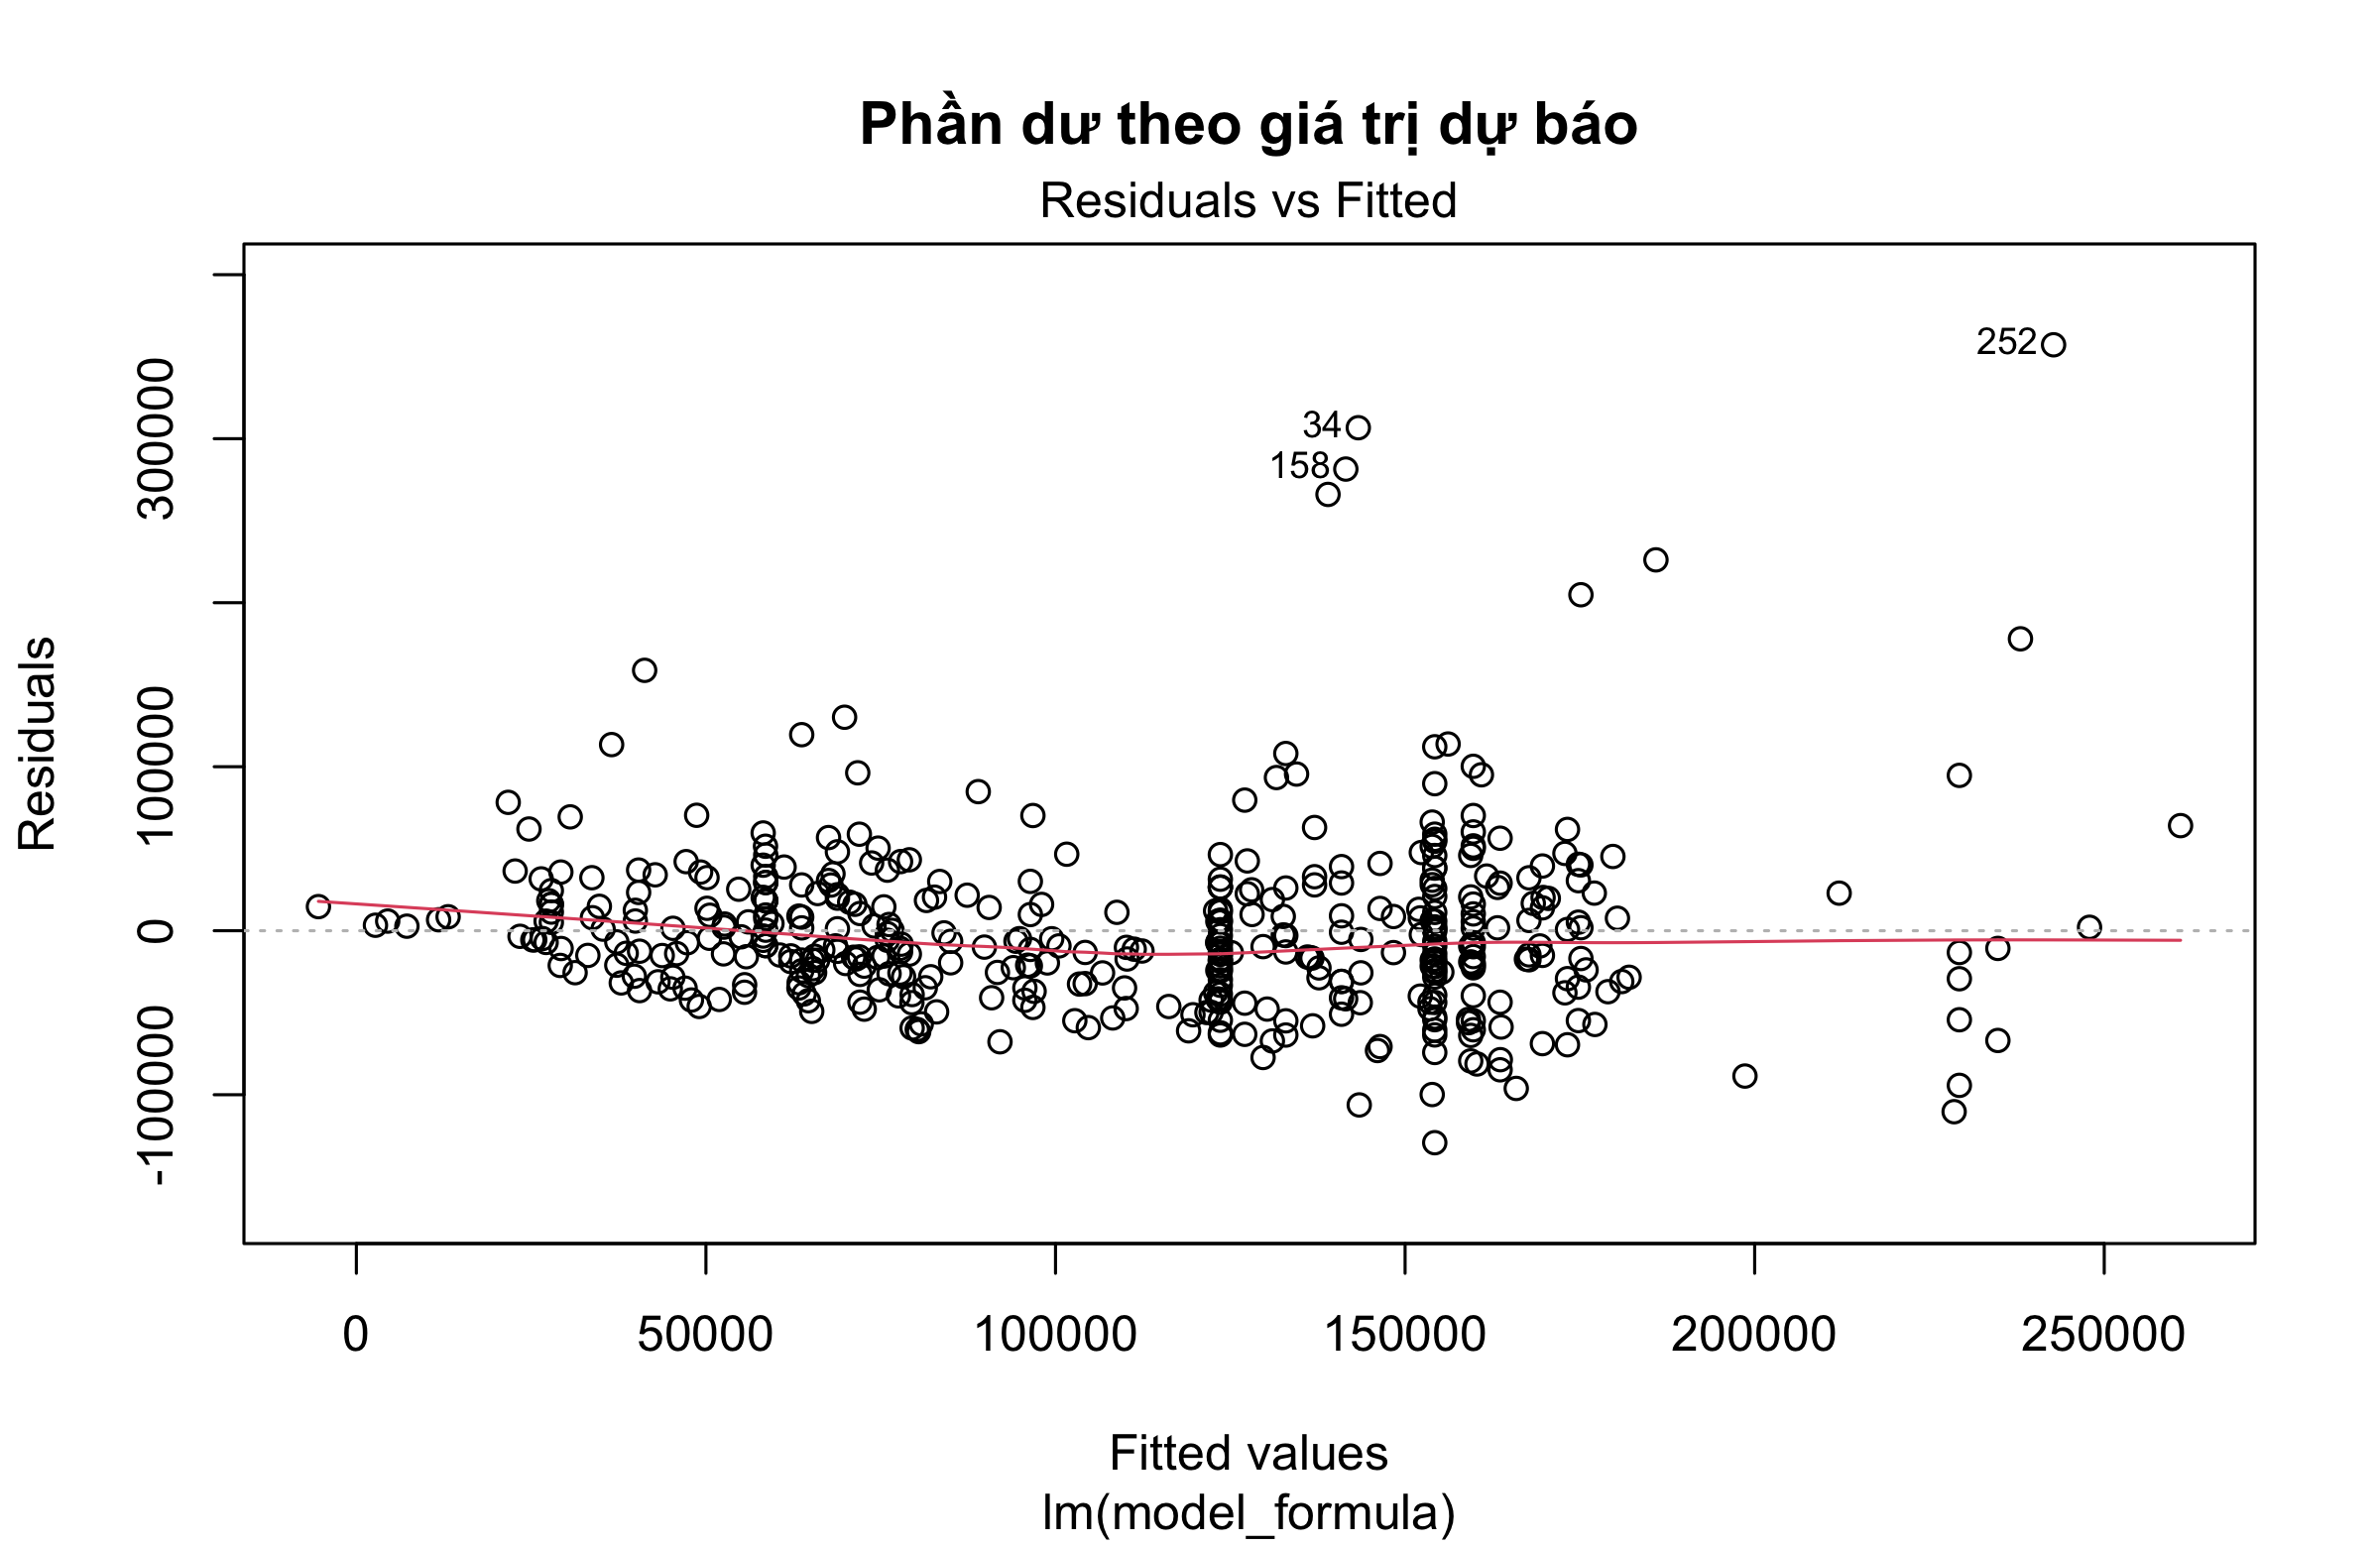
\includegraphics[width=1\linewidth]{img/nghi-ols-residuals-fitted-1.png} \end{center}

Phần dư xuất hiện ở cả hai phía của đường 0, nhưng đường làm trơn không
hoàn toàn nằm ngang: phần dư có xu hướng dương ở vùng dự báo thấp,
chuyển sang âm ở vùng giữa và tăng trở lại tại vùng dự báo cao. Độ phân
tán mở rộng rõ ở các mức lương dự báo cao, gợi ý phương sai sai số chưa
hoàn toàn đồng nhất. Biểu đồ cũng cho thấy một số phần dư dương lớn nổi
bật, phù hợp với phân phối lương lệch phải và sự hiện diện của các mức
lương cao. Những mẫu hình này cho thấy đặc tả tuyến tính cộng có thể
chưa biểu diễn hết cấu trúc dữ liệu, nhưng việc lựa chọn mô hình vẫn dựa
chủ yếu trên hiệu quả ở validation set.

\begin{center}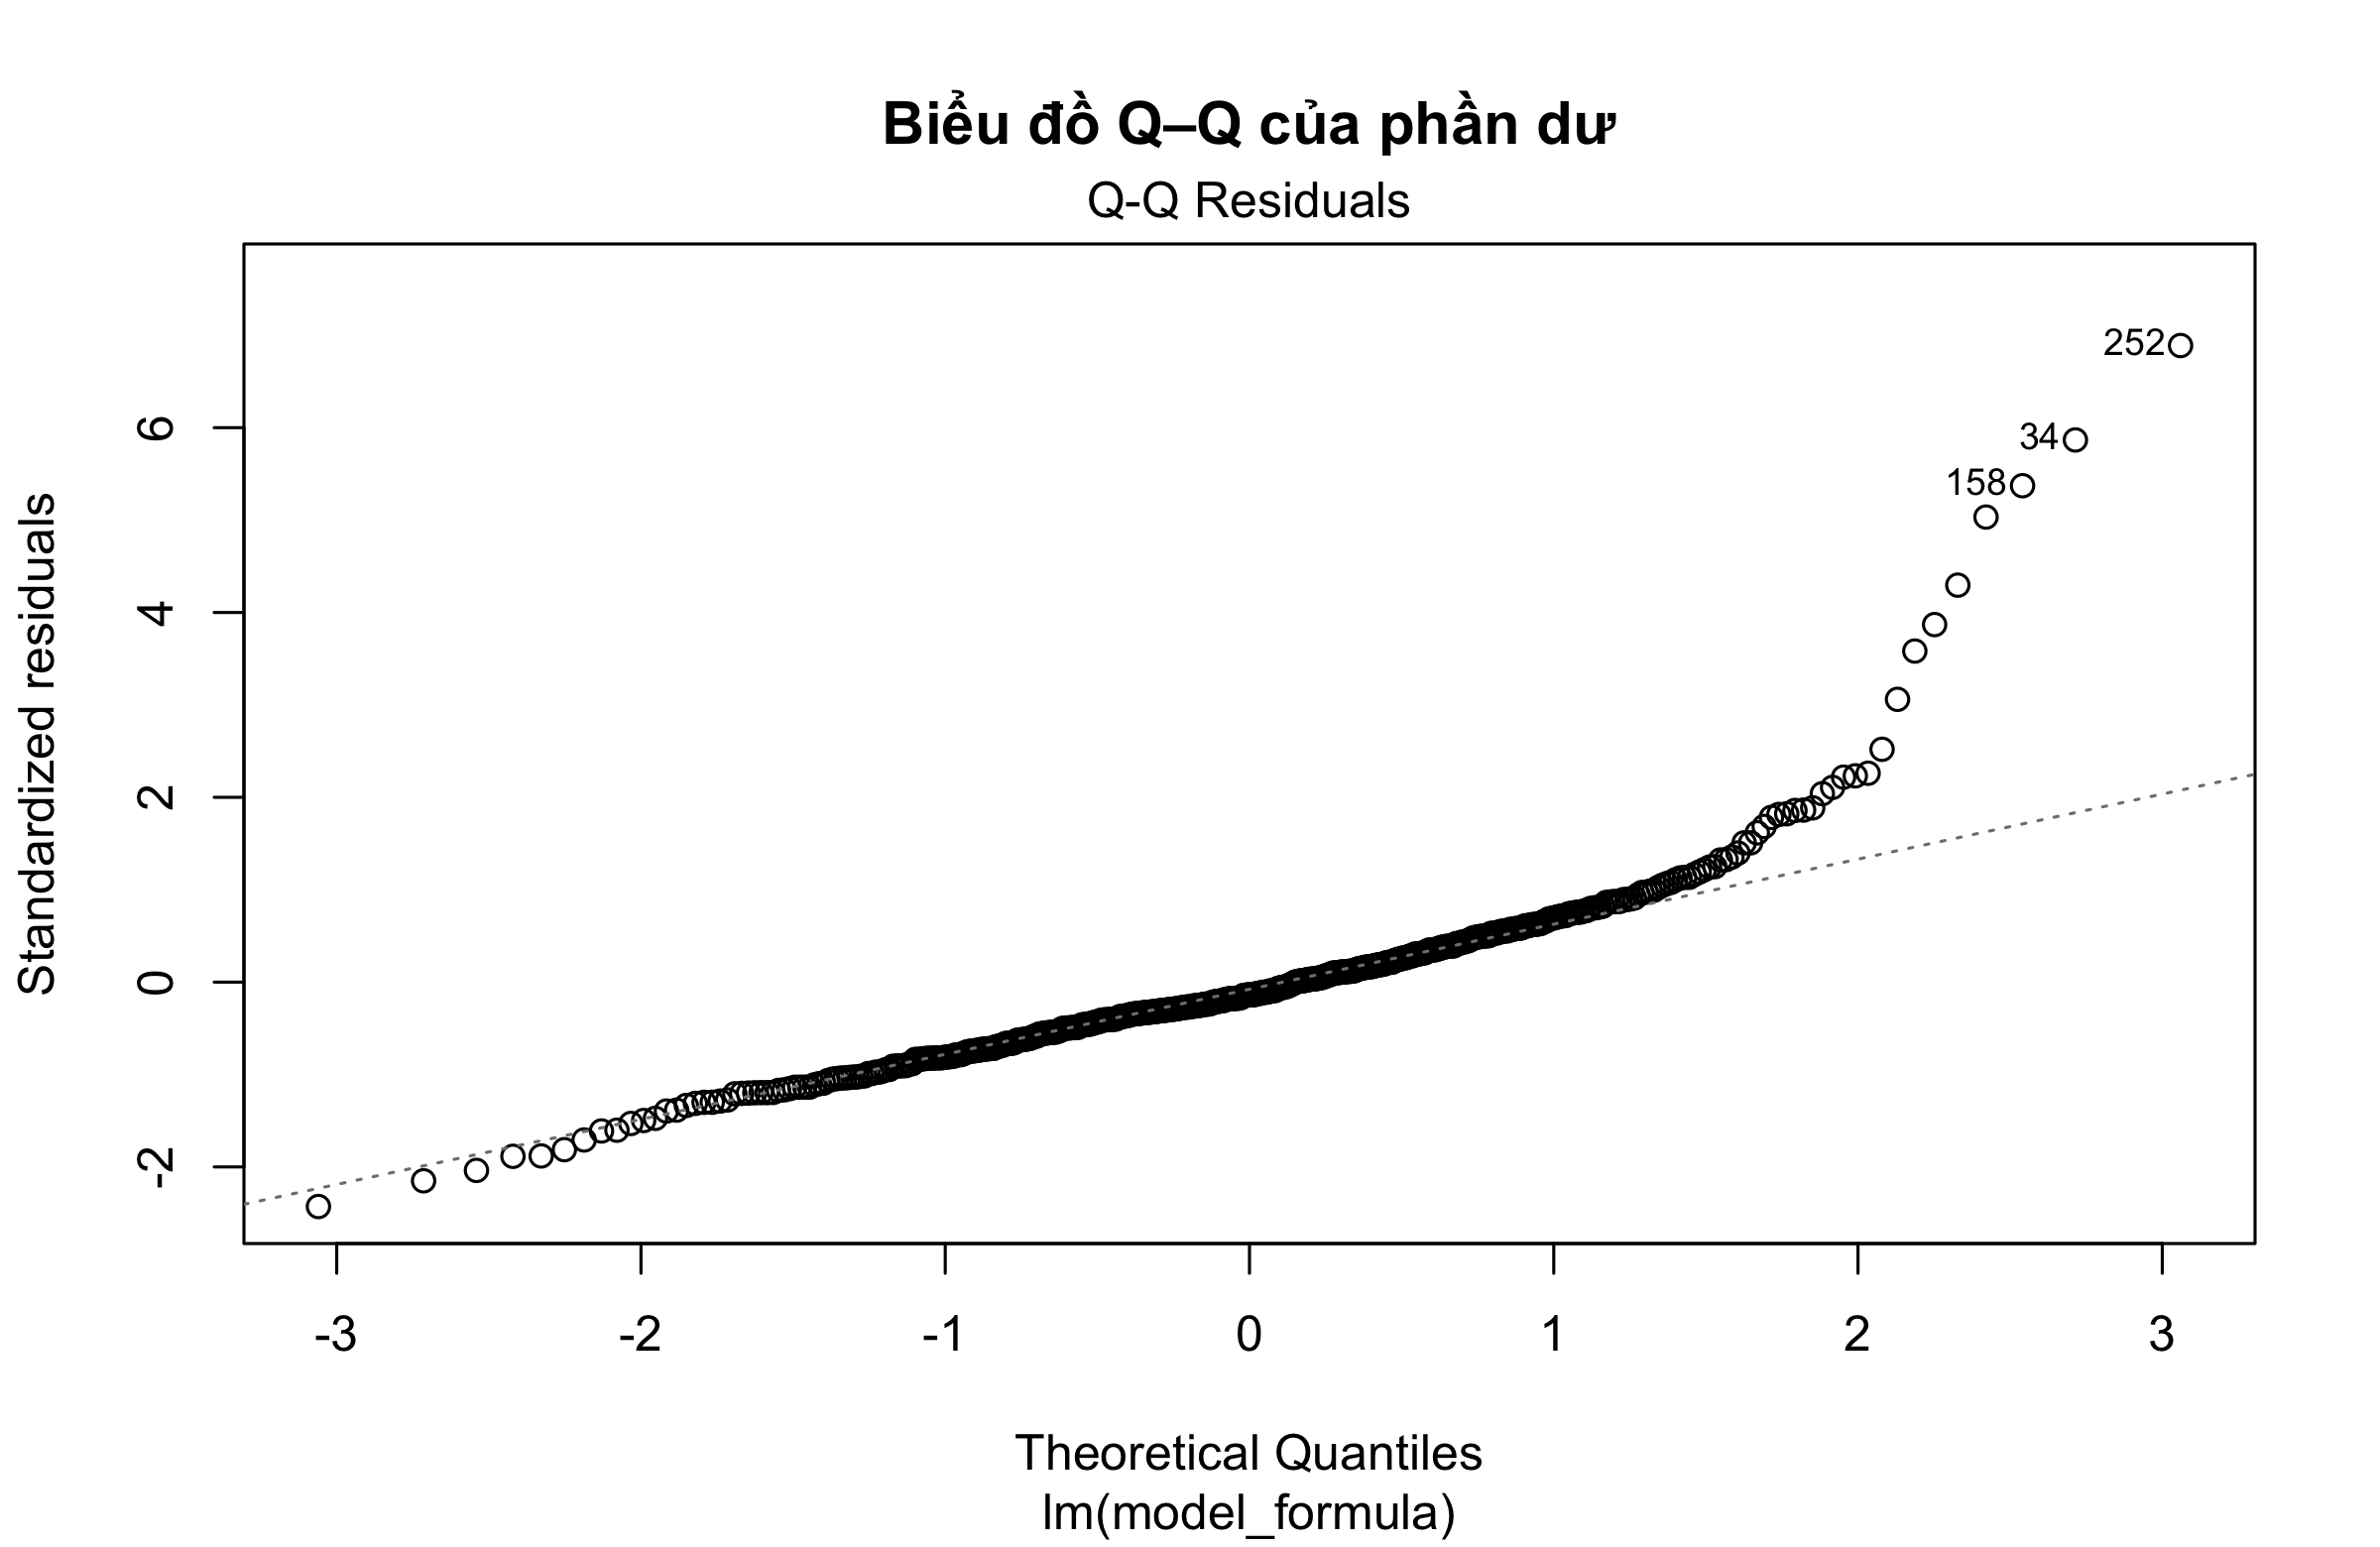
\includegraphics[width=1\linewidth]{img/nghi-ols-normal-qq-1.png} \end{center}

Trên biểu đồ Q--Q, các điểm ở phần trung tâm bám tương đối gần đường
tham chiếu, trong khi sai lệch rõ hơn tại hai đuôi và đặc biệt mạnh ở
phía phần dư dương lớn. Mẫu hình này cho thấy phần dư có đuôi phải nặng
và chưa hoàn toàn tuân theo phân phối chuẩn, có khả năng liên quan đến
một số quan sát lương cao. Kết quả không làm OLS mất vai trò mô hình
nền, nhưng yêu cầu thận trọng khi diễn giải các kết quả suy luận thống
kê. Do phần dư chưa đáp ứng hoàn toàn các giả định của OLS, p-value,
F-test và Type II ANOVA được sử dụng để hỗ trợ diễn giải mối liên hệ
thống kê, không phải làm tiêu chí lựa chọn mô hình; khả năng dự báo được
đánh giá chủ yếu bằng RMSE, MAE, MAPE và \(R^2\) trên validation set.

\subsubsection{Hồi quy điều chuẩn bằng Ridge Regression và LASSO
Regression}\label{nghi:hux1ed3i-quy-ux111iux1ec1u-chuux1ea9n-bux1eb1ng-ridge-regression-vuxe0-lasso-regression}

\textbf{Ridge Regression.}

\begin{verbatim}
##     lambda_min        cvm_min        CV_RMSE 
##       2601.676 3043462528.028      55167.586
\end{verbatim}

\texttt{alpha\ =\ 0} xác định Ridge Regression. \texttt{lambda.min} bằng
2.601,676 tại MSE cross-validation nhỏ nhất, tương ứng CV-RMSE khoảng
\$55,168. Giá trị này được chọn vì mục tiêu chính là giảm sai số dự báo
trong training set.

\begin{verbatim}
## 18 x 1 sparse Matrix of class "dgCMatrix"
##                                                  lambda.min
## (Intercept)                                     123130.0123
## work_year2021                                   -10397.0294
## work_year2022                                    -7420.2032
## experience_levelMid-level / Intermediate         13537.5064
## experience_levelSenior-level / Expert            40812.4022
## experience_levelExecutive-level / Director      112703.1070
## employment_groupOther employment arrangements     4348.0370
## job_fieldData Engineering & Architecture         -4880.2317
## job_fieldData Analytics & Business Intelligence -34601.8497
## job_fieldMachine Learning & AI                    2836.1567
## remote_ratioHybrid (50%)                         -8912.4612
## remote_ratioFully remote (100%)                   1132.9248
## company_sizeMedium                                 686.9866
## company_sizeLarge                                16322.8955
## employee_regionEurope                           -64467.6568
## employee_regionAsia                             -79872.6822
## employee_regionOthers                           -76422.6477
## same_countryKhác quốc gia                          405.1500
\end{verbatim}

Điều chuẩn L2 của Ridge Regression không đưa hệ số biến giả nào về đúng
0 tại giá trị lambda đã lựa chọn. Nhóm người lao động có cấp kinh nghiệm
Executive-level / Director có hệ số dương lớn nhất (\$112,703), trong
khi người lao động cư trú tại châu Á có hệ số âm với độ lớn lớn nhất
(\$79,873) so với người lao động cư trú tại Bắc Mỹ. Các hệ số này mô tả
đóng góp dự báo sau điều chuẩn và không đi kèm p-value theo cách ước
lượng OLS.

\textbf{LASSO Regression.}

\begin{verbatim}
##     lambda_min        cvm_min        CV_RMSE 
##       1207.591 3008167090.774      54846.760
\end{verbatim}

\texttt{alpha\ =\ 1} xác định LASSO Regression. \texttt{lambda.min} bằng
1.207,591 tại sai số cross-validation nhỏ nhất, tương ứng CV-RMSE khoảng
\$54,847. Cấu hình này được chọn theo mục tiêu giảm sai số dự báo trong
training set.

\begin{verbatim}
## 18 x 1 sparse Matrix of class "dgCMatrix"
##                                                 lambda.min
## (Intercept)                                     122540.172
## work_year2021                                    -2648.011
## work_year2022                                        .    
## experience_levelMid-level / Intermediate          6371.163
## experience_levelSenior-level / Expert            33939.368
## experience_levelExecutive-level / Director      104627.372
## employment_groupOther employment arrangements        .    
## job_fieldData Engineering & Architecture         -1579.898
## job_fieldData Analytics & Business Intelligence -31965.333
## job_fieldMachine Learning & AI                       .    
## remote_ratioHybrid (50%)                         -5847.552
## remote_ratioFully remote (100%)                      .    
## company_sizeMedium                                   .    
## company_sizeLarge                                14028.750
## employee_regionEurope                           -63764.727
## employee_regionAsia                             -78697.448
## employee_regionOthers                           -72803.910
## same_countryKhác quốc gia                            .
\end{verbatim}

Trong LASSO Regression, nhóm người lao động có cấp kinh nghiệm
Executive-level / Director có hệ số dương lớn nhất, còn người lao động
cư trú tại châu Á có hệ số âm với độ lớn lớn nhất so với các mức tham
chiếu tương ứng. Mô hình đưa 6 hệ số biến giả về 0; các hệ số còn lại
nhìn chung giữ cùng chiều với OLS và Ridge Regression nhưng chịu mức co
khác nhau. Một hệ số biến giả bằng 0 không đồng nghĩa toàn bộ biến phân
loại bị loại; chỉ khi mọi hệ số đại diện cho biến đó đều bằng 0 mới có
thể kết luận biến không được giữ trong cấu trúc dự báo. LASSO Regression
không cung cấp p-value theo cách ước lượng OLS, nên các hệ số được diễn
giải theo đóng góp dự báo thay vì kiểm định riêng lẻ.

\subsubsection{Đánh giá và lựa chọn mô
hình}\label{nghi:ux111uxe1nh-giuxe1-vuxe0-lux1ef1a-chux1ecdn-muxf4-huxecnh}

RMSE là tiêu chí lựa chọn chính; MAE, MAPE và \(R^2\) bổ sung thông tin về độ
lớn, tỷ lệ sai số và khả năng giải thích ngoài mẫu.

\begin{verbatim}
##              Model     RMSE      MAE     MAPE        R2
## 1              OLS 53339.41 35204.30 56.99144 0.3719520
## 2 Ridge Regression 53172.54 34948.09 59.50827 0.3758754
## 3 LASSO Regression 53338.39 34934.42 62.74898 0.3719760
\end{verbatim}

\textbf{Kết luận chung về các mô hình hồi quy.}

Trên validation set, Ridge Regression có RMSE thấp nhất, bằng \$53,173,
tiếp theo là LASSO Regression với \$53,338 và OLS với \$53,339. Ridge
Regression giảm RMSE khoảng \$167 so với OLS và \$166 so với LASSO
Regression, tương ứng mức cải thiện khoảng 0,31\%. Vì vậy, Ridge
Regression được lựa chọn theo tiêu chí RMSE đã xác định trước, nhưng
khoảng cách này quá nhỏ để kết luận mô hình vượt trội về mặt thực tiễn.
LASSO Regression có MAE thấp nhất, Ridge Regression có \(R^2\) cao nhất và
OLS có MAPE thấp nhất; không mô hình nào cho kết quả tốt nhất ở toàn bộ
chỉ số.

Nhìn chung, cả ba mô hình tạo ra khả năng dự báo ở mức vừa phải và có
thể được sử dụng làm các mô hình nền. \(R^2\) và \(R^2\) hiệu chỉnh của mô hình
OLS trên training set lần lượt bằng 0,489 và 0,469, phản ánh mức độ phù
hợp trong dữ liệu dùng để ước lượng. Các giá trị \(R^2\) từ 0,372 đến 0,376
trên validation set cho thấy các biến đầu vào giải thích được hơn một
phần ba biến thiên mức lương ngoài mẫu so với phương án dùng mức lương
trung bình thực tế của validation set làm dự báo cho mọi quan sát. MAE
khoảng \$35,000 và RMSE khoảng \$53,000 cho thấy sai số dự báo vẫn còn
đáng kể, do đó các mô hình mới nhận diện được một phần cấu trúc của mức
lương. Trong bối cảnh mức lương trung vị của toàn bộ mẫu là \$100,000,
quy mô MAE và RMSE cho thấy độ lệch dự báo không nhỏ.

Hiệu quả gần tương đương giữa OLS, Ridge Regression và LASSO Regression
có thể liên quan đến việc ba mô hình sử dụng cùng tập biến đầu vào và
cùng cấu trúc tuyến tính cộng. Ridge Regression và LASSO Regression thay
đổi cách ước lượng hệ số thông qua điều chuẩn nhưng không bổ sung thông
tin mới, quan hệ phi tuyến hoặc thành phần tương tác. Bên cạnh đó, các
GVIF hiệu chỉnh đều gần 1 và 17 biến sau mã hóa không lớn so với 452
quan sát trong training set, nên lợi ích của điều chuẩn đối với đa cộng
tuyến và độ phức tạp mô hình có khả năng bị giới hạn. Phân phối mức
lương lệch phải, có độ phân tán lớn và vẫn giữ các mức lương ngoại lai
hợp lý, khiến RMSE nhạy với một số sai số lớn. Dữ liệu đầu vào chủ yếu
gồm các nhóm phân loại tương đối rộng và không có những thông tin chi
tiết như số năm kinh nghiệm thực tế, trình độ học vấn, kỹ năng chuyên
môn, quốc gia hoặc thành phố cụ thể, ngành hoạt động và đặc điểm riêng
của doanh nghiệp; sự thiếu vắng này có thể giới hạn khả năng giải thích
và dự báo của cả ba mô hình. Kết quả cũng dựa trên một lần chia
training--validation, vì vậy mức chênh lệch rất nhỏ giữa ba mô hình
không nên được diễn giải quá mức.

Mặc dù Ridge Regression được lựa chọn làm mô hình hồi quy đại diện theo
tiêu chí RMSE, OLS vẫn phù hợp hơn cho việc diễn giải các đặc điểm liên
hệ với mức lương vì hệ số được trình bày trực tiếp theo nhóm tham chiếu
và đi kèm các kết quả suy luận thống kê. Như đã trình bày trong phần
OLS, cấp kinh nghiệm và khu vực cư trú là hai nhóm đặc điểm tạo ra chênh
lệch rõ nhất, tiếp theo là lĩnh vực nghề nghiệp và quy mô công ty. Các
hệ số của Ridge nhìn chung giữ nguyên chiều và thứ tự tương đối của
những mẫu hình chính sau điều chuẩn, cho thấy kết luận không phụ thuộc
hoàn toàn vào một phương pháp ước lượng duy nhất. Tuy nhiên, các hệ số
chỉ phản ánh mối liên hệ sau khi đồng thời xét các biến còn lại, không
phải tác động nhân quả.

OLS có ưu điểm lớn nhất về khả năng diễn giải và suy luận thống kê thông
qua hệ số, p-value, F-test và Type II ANOVA, nhưng không điều chuẩn hệ
số và bị giới hạn bởi cấu trúc tuyến tính cộng. Ridge Regression cải
thiện độ ổn định thông qua khoản phạt L2 và đạt RMSE thấp nhất, song mức
cải thiện chỉ khoảng 0,31\%, mô hình vẫn giữ toàn bộ biến và các hệ số
không đi kèm p-value theo cách ước lượng OLS. LASSO Regression tạo mô
hình gọn hơn khi đưa 6 hệ số biến giả về 0, nhưng việc loại từng mức
riêng lẻ khó diễn giải ở cấp toàn bộ biến phân loại và RMSE gần như
không khác OLS. Điểm hạn chế chung của ba mô hình là cùng dựa trên các
hiệu ứng tuyến tính cộng, trong khi EDA cho thấy chênh lệch mức lương có
thể thay đổi theo sự kết hợp giữa kinh nghiệm, lĩnh vực nghề nghiệp, khu
vực và hình thức làm việc. Vì vậy, CatBoost được xây dựng ở phần tiếp
theo để đánh giá liệu một mô hình dựa trên cây, có khả năng xử lý trực
tiếp biến phân loại và biểu diễn các quan hệ phức tạp hơn, có cải thiện
khả năng dự báo ngoài mẫu so với Ridge Regression hay không. CatBoost
không được mặc định là tốt hơn; mô hình phải được đánh giá trên cùng
validation set và cùng các chỉ số để bảo đảm so sánh nhất quán.

\subsection{Xây dựng và đánh giá mô hình
CatBoost}\label{nghi:xuxe2y-dux1ef1ng-vuxe0-ux111uxe1nh-giuxe1-muxf4-huxecnh-catboost}

\subsubsection{Phương pháp triển khai
CatBoost}\label{nghi:phux1b0ux1a1ng-phuxe1p-triux1ec3n-khai-catboost}

Sau khi các mô hình hồi quy tuyến tính cho kết quả dự báo tương đối gần
nhau, CatBoost được sử dụng để đánh giá liệu một mô hình dựa trên cây có
thể khai thác thêm các quan hệ phi tuyến và sự kết hợp giữa các đặc điểm
hay không. Việc sử dụng CatBoost phù hợp với bộ dữ liệu hiện tại vì toàn
bộ tám biến dự báo đều là biến phân loại. Mô hình được triển khai trên
cùng phép chia dữ liệu và cùng thang lương USD để kết quả có thể so sánh
trực tiếp với OLS, Ridge Regression và LASSO Regression.

CatBoost là mô hình gradient boosting trên cây quyết định. Mô hình bắt
đầu từ một dự báo nền rồi xây dựng nhiều cây theo trình tự; mỗi cây mới
tập trung điều chỉnh phần sai số còn lại của tập hợp cây đã có. Dự báo
cuối cùng là tổng đóng góp của toàn bộ các cây, còn tốc độ học giới hạn
mức độ mỗi cây được phép thay đổi dự báo chung. Khác với cấu trúc tuyến
tính cộng của ba mô hình hồi quy, các nhánh cây có thể sử dụng những tổ
hợp khác nhau giữa cấp kinh nghiệm, lĩnh vực nghề nghiệp, khu vực cư trú
và các đặc điểm khác, nhưng tính linh hoạt này không bảo đảm mọi quan hệ
được học đều khái quát tốt trên dữ liệu mới.

Việc xử lý biến phân loại và Ordered boosting là hai thành phần có liên
quan nhưng không đồng nhất. Các cột factor cho phép CatBoost xây dựng
biểu diễn biến phân loại bên trong thuật toán, trong đó các thống kê
liên quan đến biến mục tiêu có thể được hình thành theo thứ tự quan sát
nhằm hạn chế việc dùng thông tin của một quan sát để mã hóa chính nó.
Đồng thời, \texttt{boosting\_type\ =\ "Ordered"} áp dụng nguyên tắc thứ
tự trong chuỗi boosting để hạn chế \emph{prediction shift} (độ lệch giữa
dự báo trong quá trình học và trên dữ liệu mới). Hai thành phần này hỗ
trợ kiểm soát rò rỉ biến mục tiêu và quá khớp nhưng không loại bỏ hoàn
toàn các rủi ro đó \cite{prokhorenkova2018,catboost_docs}.

Trong quá trình triển khai, CatBoost sử dụng lại đúng training set và
validation set đã được tạo ở Phần 6. Khác với Ridge Regression và LASSO
Regression, dữ liệu không được chuyển qua \texttt{model.matrix()} vì tám
biến dự báo được giữ ở dạng factor và được xử lý bên trong mô hình. Đoạn
code dưới đây kiểm tra package, ghi nhận phiên bản thực tế và tách biến
mục tiêu khỏi tập đặc trưng.

\begin{verbatim}
## [1] '1.2.10'
\end{verbatim}

Package CatBoost được sử dụng ở phiên bản 1.2.10. Training set gồm 452
quan sát, validation set gồm 113 quan sát và cả hai có đúng tám biến dự
báo theo cùng thứ tự cột. Biến mục tiêu \texttt{salary\_in\_usd} được
lưu riêng trên thang USD gốc và không nằm trong tập đặc trưng đầu vào.

Dữ liệu được tổ chức thành Pool sau khi xác nhận toàn bộ cột đầu vào vẫn
là factor. Pool là cấu trúc dữ liệu của CatBoost, trong đó đặc trưng và
nhãn được đóng gói để phục vụ huấn luyện hoặc dự báo; việc tạo Pool chưa
làm phát sinh quá trình học mô hình \cite{catboost_docs}.

Cấu trúc Pool giữ nguyên biểu diễn phân loại thay vì one-hot encode thủ
công. Điều này không có nghĩa dữ liệu không được chuyển đổi, mà cho phép
CatBoost tự xác định cách biểu diễn biến phân loại trong quá trình huấn
luyện. Validation Pool có chứa nhãn để tính các chỉ số sau dự báo, nhưng
nhãn này không được sử dụng để ước lượng mô hình cuối cùng.

\subsubsection{Điều chỉnh siêu tham số bằng
cross-validation}\label{nghi:ux111iux1ec1u-chux1ec9nh-siuxeau-tham-sux1ed1-bux1eb1ng-cross-validation}

Hiệu quả của CatBoost phụ thuộc vào mức độ phức tạp của cây, tốc độ cập
nhật dự báo và mức điều chuẩn. Vì training set chỉ có 452 quan sát,
nghiên cứu sử dụng một lưới siêu tham số có phạm vi giới hạn nhằm cân
bằng giữa khả năng học cấu trúc dữ liệu và nguy cơ quá khớp. Độ sâu cây
kiểm soát số lớp phân chia và do đó ảnh hưởng trực tiếp đến khả năng
biểu diễn những tổ hợp đặc điểm phức tạp. Tốc độ học xác định mức đóng
góp của mỗi cây vào dự báo chung, trong khi hệ số điều chuẩn tại lá làm
co các giá trị dự báo tại lá để hạn chế những điều chỉnh quá cực đoan.

Số cây không được đưa trực tiếp vào lưới. Trong mỗi fold, mô hình được
phép xây dựng tối đa 1.500 cây, nhưng early stopping dừng quá trình nếu
RMSE không còn cải thiện trong 50 vòng. Cách thiết kế này cho phép số
cây thích ứng với từng phần dữ liệu đánh giá nội bộ thay vì áp đặt trước
một giá trị duy nhất \cite{catboost_docs}.

\begin{verbatim}
##    depth learning_rate l2_leaf_reg
## 1      4          0.03           3
## 2      6          0.03           3
## 3      8          0.03           3
## 4      4          0.05           3
## 5      6          0.05           3
## 6      8          0.05           3
## 7      4          0.03           7
## 8      6          0.03           7
## 9      8          0.03           7
## 10     4          0.05           7
## 11     6          0.05           7
## 12     8          0.05           7
\end{verbatim}

Lưới gồm 12 cấu hình, kết hợp độ sâu cây 4, 6 hoặc 8; tốc độ học 0,03
hoặc 0,05; và hệ số điều chuẩn tại lá 3 hoặc 7. Phạm vi này đối chiếu
cây tương đối đơn giản với cây có khả năng tạo nhiều phân chia hơn, đồng
thời xem xét hai mức cập nhật và hai mức điều chuẩn. Đây là một lưới có
kiểm soát phù hợp với quy mô training set, không phải tìm kiếm toàn
diện; vì vậy các cấu hình ngoài lưới chưa được đánh giá.

Đối với mỗi cấu hình, training set được đánh giá bằng 10-fold
cross-validation theo chính vector phân chia đã sử dụng cho Ridge
Regression và LASSO Regression. Mô hình được huấn luyện 10 lần, mỗi lần
dùng chín fold để học và một fold để đánh giá nội bộ; trung bình RMSE
của 10 lần đại diện cho cấu hình. Fold đánh giá nội bộ cũng theo dõi
early stopping, nên khác hoàn toàn với validation set gồm 113 quan sát
được giữ lại cho đánh giá ngoài mẫu. Tùy chọn
\texttt{use\_best\_model\ =\ TRUE} giữ mô hình tại vòng có RMSE tốt nhất
trong fold đánh giá nội bộ thay vì giữ toàn bộ 1.500 cây.

\begin{verbatim}
##    depth learning_rate l2_leaf_reg  CV_RMSE CV_RMSE_SD selected_iterations
## 1      8          0.05           3 51617.85   11884.17                 154
## 2      6          0.05           7 51633.08   12247.74                 160
## 3      8          0.03           3 51717.35   12094.17                 233
## 4      4          0.05           3 51783.62   11514.11                 160
## 5      6          0.03           7 51847.42   11760.44                 262
## 6      4          0.05           7 52031.40   12816.05                 140
## 7      6          0.05           3 52085.80   11946.12                 147
## 8      8          0.03           7 52137.18   12075.16                 240
## 9      8          0.05           7 52148.15   12310.90                 158
## 10     6          0.03           3 52196.45   11832.60                 208
## 11     4          0.03           7 52217.65   11745.11                 284
## 12     4          0.03           3 52328.78   12286.03                 276
\end{verbatim}

Kết quả cross-validation cho thấy cấu hình có độ sâu cây bằng 8, tốc độ
học 0,05 và điều chuẩn tại lá bằng 3 đạt CV-RMSE thấp nhất, khoảng
\$51,618. Cấu hình đứng thứ hai sử dụng độ sâu cây bằng 6, tốc độ học
0,05 và điều chuẩn tại lá bằng 7, với CV-RMSE khoảng \$51,633; chênh
lệch chỉ khoảng \$15. Một cấu hình có độ sâu cây bằng 4 đạt CV-RMSE
khoảng \$51,784, cao hơn cấu hình đứng đầu khoảng \$166.

Những chênh lệch này nhỏ hơn nhiều so với độ lệch chuẩn RMSE giữa các
fold, vốn nằm quanh \$11,500--\$12,800. Thứ hạng cấu hình vì vậy có độ
nhạy đáng kể với phần dữ liệu đảm nhiệm vai trò đánh giá nội bộ. Độ sâu
cây bằng 8 được chọn theo tiêu chí CV-RMSE nhỏ nhất đã xác định trước,
nhưng kết quả không cho thấy cấu hình này vượt trội rõ ràng so với các
cây đơn giản hơn. Độ lệch chuẩn giữa các fold phản ánh độ phân tán của
10 kết quả RMSE, không phải sai số chuẩn của CV-RMSE trung bình.

Các cấu hình có tốc độ học 0,05 nhìn chung cần ít cây hơn các cấu hình
có tốc độ học 0,03, phù hợp với việc mỗi cây đóng góp nhiều hơn vào dự
báo chung. Kết quả cũng không cho phép kết luận một giá trị điều chuẩn
tại lá luôn tốt hơn giá trị còn lại, vì hiệu quả phụ thuộc đồng thời vào
độ sâu cây và tốc độ học. CV-RMSE không được so sánh trực tiếp với RMSE
trên validation set như hai kết quả được tính trên cùng một tập quan
sát.

Cấu hình có CV-RMSE nhỏ nhất được tách ra để xác định siêu tham số và số
cây đại diện cho mô hình sẽ huấn luyện trên toàn bộ training set.

\begin{verbatim}
##   depth learning_rate l2_leaf_reg  CV_RMSE CV_RMSE_SD selected_iterations
## 1     8          0.05           3 51617.85   11884.17                 154
\end{verbatim}

Cấu hình được lựa chọn có độ sâu cây bằng 8, tốc độ học 0,05, điều chuẩn
tại lá bằng 3 và CV-RMSE khoảng \$51,618; độ lệch chuẩn RMSE giữa các
fold là \$11,884. Số cây của mô hình cuối cùng được xác định bằng trung
vị số cây được giữ lại trong 10 fold, bằng 154 cây. Trung vị tạo ra một
giá trị đại diện ít nhạy hơn với một fold có số cây đặc biệt cao hoặc
thấp. Đây là quy tắc thực hành để chuyển kết quả cross-validation sang
mô hình cuối cùng, không phải bằng chứng rằng 154 là số cây tối ưu tuyệt
đối trên mọi mẫu dữ liệu.

\subsubsection{Kết quả mô hình
CatBoost}\label{nghi:kux1ebft-quux1ea3-muxf4-huxecnh-catboost}

Cấu hình được lựa chọn từ cross-validation được sử dụng để huấn luyện
lại mô hình trên toàn bộ 452 quan sát của training set. Việc huấn luyện
lại cho phép mô hình sử dụng toàn bộ thông tin trong training set sau
khi các siêu tham số và số cây đã được cố định. Bảng dưới đây tổng hợp
cấu hình được chuyển sang mô hình cuối cùng.

\begin{verbatim}
##   depth learning_rate l2_leaf_reg iterations boosting_type task_type
## 1     8          0.05           3        154       Ordered       CPU
\end{verbatim}

Độ sâu cây bằng 8 cho phép mỗi cây có tám lớp phân chia, trong khi tốc
độ học 0,05 giới hạn đóng góp của từng cây ở mức tương đối thận trọng.
Hệ số điều chuẩn tại lá bằng 3 làm co các giá trị dự báo tại lá, còn 154
iterations xác định mô hình gồm 154 cây. Ordered boosting được sử dụng
trong toàn bộ quá trình và việc huấn luyện trên CPU giúp quy trình dễ
tái lập trong môi trường hiện tại.

Mô hình cuối cùng không nhận một Pool đánh giá nội bộ và đặt
\texttt{use\_best\_model\ =\ FALSE} vì số cây đã được xác định từ
cross-validation. Nếu validation set được dùng để chọn lại số cây, tập
đánh giá ngoài mẫu sẽ tham gia vào quá trình học. Từ cấu hình đã cố
định, mô hình được huấn luyện lại và tạo dự báo như sau.

Validation set chỉ được đưa qua mô hình sau khi quá trình huấn luyện đã
hoàn tất. Các dự báo được giữ ở độ chính xác đầy đủ, không làm tròn
trước khi tính RMSE, MAE, MAPE và \(R^2\). Đây là lần đầu 113 quan sát
validation được sử dụng để đánh giá hiệu quả CatBoost; chúng không tham
gia lựa chọn độ sâu cây, tốc độ học, điều chuẩn tại lá, số cây hoặc
early stopping.

Ngoài hiệu quả dự báo, cấu trúc của mô hình được xem xét thông qua mức
độ quan trọng của các biến. PredictionValuesChange đo mức thay đổi trung
bình của dự báo liên quan đến việc sử dụng một biến trong toàn bộ tập
hợp cây; biến tạo ra các phân chia làm dự báo thay đổi nhiều hơn sẽ nhận
điểm importance cao hơn \cite{catboost_docs}. Tên các biến được chuyển sang
nhãn tiếng Việt trong output để bảng và biểu đồ dễ đọc hơn.

\begin{verbatim}
##                   Variable Importance
## 1           Khu vực cư trú 41.3338736
## 2          Cấp kinh nghiệm 33.5820157
## 3     Lĩnh vực nghề nghiệp 10.0938509
## 4           Quy mô công ty  7.1369026
## 5             Năm làm việc  5.5724609
## 6       Hình thức làm việc  1.1167404
## 7 Trạng thái cùng quốc gia  0.7954835
## 8          Nhóm tuyển dụng  0.3686723
\end{verbatim}

Bảng sắp xếp tám biến theo điểm importance giảm dần. Biểu đồ thanh ngang
trình bày lại chính các giá trị này nhằm làm rõ thứ hạng tương đối,
không tạo thêm một thước đo khác.

\begin{center}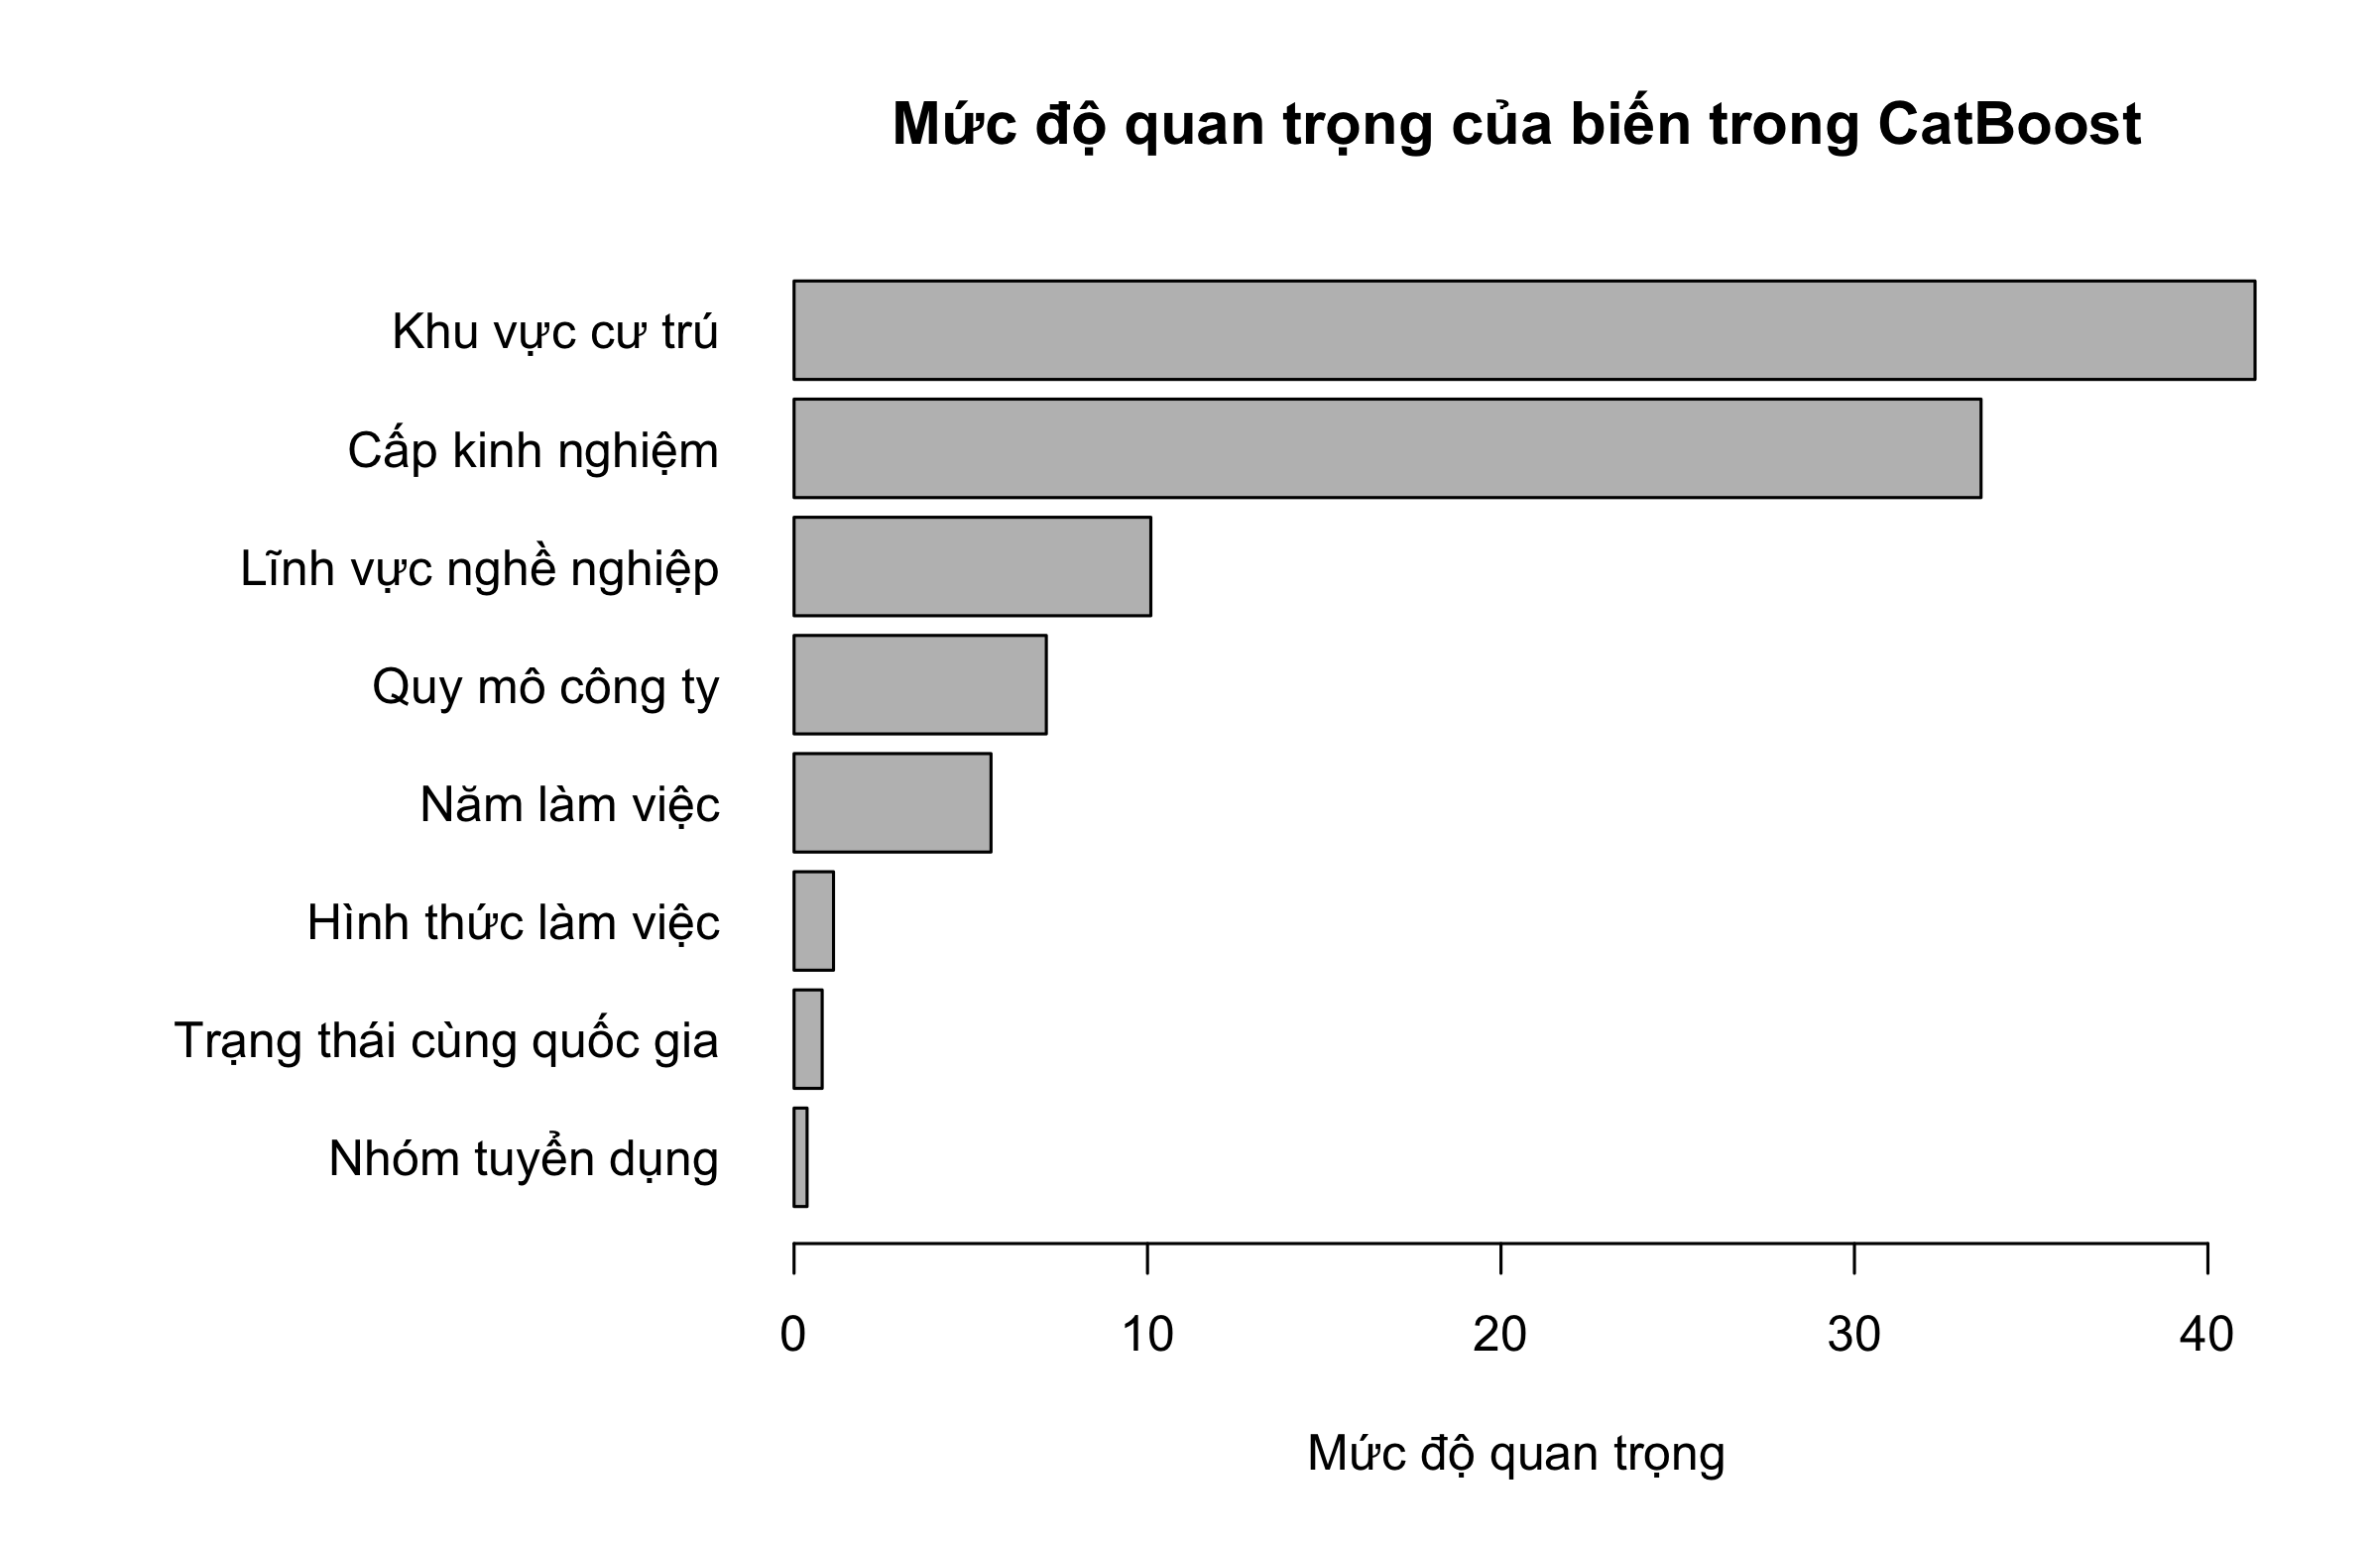
\includegraphics[width=1\linewidth]{img/nghi-catboost-feature-importance-plot-1.png} \end{center}

Khu vực cư trú có mức độ quan trọng cao nhất, bằng 41,33, tiếp theo là
cấp kinh nghiệm với 33,58 và lĩnh vực nghề nghiệp với 10,09. Ba biến này
chiếm phần lớn tổng điểm quan trọng của mô hình. Quy mô công ty và năm
làm việc đứng ở nhóm tiếp theo, trong khi hình thức làm việc, trạng thái
cùng quốc gia và nhóm tuyển dụng có mức độ quan trọng thấp hơn.

Thứ hạng này nhất quán với OLS và EDA ở việc khu vực cư trú cùng cấp
kinh nghiệm là hai nhóm thông tin nổi bật nhất. Lĩnh vực nghề nghiệp
tiếp tục có vai trò đáng kể, trong khi CatBoost dành thêm một phần thông
tin cho quy mô công ty và năm làm việc. Kết quả có thể phản ánh khả năng
CatBoost sử dụng các biến trong những tổ hợp phân chia khác nhau, nhưng
chưa đủ để xác định cụ thể tổ hợp nào tạo ra chênh lệch dự báo.

Giá trị 41,33 của khu vực cư trú không có nghĩa biến này giải thích
41,33\% biến thiên của mức lương. PredictionValuesChange không cho biết
khu vực nào có mức lương cao hoặc thấp hơn, không có đơn vị USD, không
đi kèm p-value và không phải bằng chứng về quan hệ nhân quả. Chiều và độ
lớn của các chênh lệch giữa nhóm vẫn được diễn giải chủ yếu từ OLS;
feature importance không được dùng để loại biến hoặc chạy lại CatBoost.

\subsubsection{Đánh giá ngoài mẫu và thảo
luận}\label{nghi:ux111uxe1nh-giuxe1-ngouxe0i-mux1eabu-vuxe0-thux1ea3o-luux1eadn}

Khả năng dự báo của mô hình được đánh giá trên 113 quan sát thuộc
validation set, sử dụng cùng RMSE, MAE, MAPE và \(R^2\) như các mô hình hồi
quy. Bốn chỉ số được tính từ dự báo chưa làm tròn và mức lương thực tế
trên thang USD gốc.

\begin{verbatim}
##      Model     RMSE      MAE     MAPE        R2
## 1 CatBoost 52942.54 34824.35 60.85503 0.3812631
\end{verbatim}

Trên validation set, CatBoost đạt RMSE khoảng \$52,943 và MAE khoảng
\$34,824. RMSE đặt trọng số lớn hơn cho các sai số lớn, trong khi MAE
cho biết độ lệch tuyệt đối trung bình giữa dự báo và mức lương thực tế
vào khoảng \$34,824. \(R^2\) bằng 0,3813 cho thấy mô hình giải thích được
khoảng 38,1\% biến thiên mức lương ngoài mẫu so với phương án dùng mức
lương trung bình thực tế của validation set làm dự báo cho mọi quan sát.

MAPE bằng 60,86\% tương đối cao và cần được đọc thận trọng vì chỉ số
nhạy với các quan sát có mức lương thực tế thấp. Kết quả cho thấy việc
đạt RMSE thấp nhất không đồng nghĩa CatBoost có sai số tỷ lệ tốt nhất ở
mọi phân đoạn mức lương. RMSE trên validation set cao hơn CV-RMSE trung
bình khoảng \$1,325; hai giá trị được tính trên các tập quan sát khác
nhau nên không tạo thành một phép kiểm định trực tiếp. Chênh lệch này
không lớn so với độ lệch chuẩn giữa các fold, cho thấy kết quả
validation chưa tách rời hoàn toàn mức hiệu quả quan sát được trong
cross-validation.

Bảng tổng hợp giữ nguyên ba kết quả hồi quy ở Phần 6 và bổ sung CatBoost
để so sánh bốn mô hình trên cùng validation set.

\begin{verbatim}
##              Model     RMSE      MAE     MAPE        R2
## 1              OLS 53339.41 35204.30 56.99144 0.3719520
## 2 Ridge Regression 53172.54 34948.09 59.50827 0.3758754
## 3 LASSO Regression 53338.39 34934.42 62.74898 0.3719760
## 4         CatBoost 52942.54 34824.35 60.85503 0.3812631
\end{verbatim}

CatBoost đạt RMSE thấp nhất và giảm khoảng \$230 so với Ridge
Regression, tương ứng 0,43\%. MAE giảm khoảng \$124 và \(R^2\) tăng từ 0,3759
lên 0,3813, nên hai chỉ số này ủng hộ CatBoost nhẹ. Ngược lại, MAPE của
CatBoost bằng 60,86\%, cao hơn 59,51\% của Ridge Regression khoảng 1,35
điểm phần trăm. Các thước đo vì vậy không tạo ra một thứ tự hoàn toàn
đồng nhất.

Mức cải thiện RMSE 0,43\% là rất nhỏ so với quy mô sai số chung khoảng
\$53,000. CatBoost và Ridge Regression nên được xem là có hiệu quả dự
báo gần tương đương trong phép chia dữ liệu hiện tại, thay vì coi độ
phức tạp của mô hình cây là một ưu thế thực tiễn rõ ràng. CatBoost được
chọn theo tiêu chí RMSE đã xác định trước, còn Ridge Regression vẫn là
phương án đơn giản hơn, dễ tái lập và phù hợp khi ưu tiên khả năng giải
thích.

Khả năng biểu diễn quan hệ phức tạp hơn không bảo đảm hiệu quả tốt hơn
khi chỉ có 452 quan sát để huấn luyện và các biến đầu vào chủ yếu là
những nhóm phân loại rộng. Những thông tin chi tiết như số năm kinh
nghiệm thực tế, kỹ năng, trình độ học vấn, địa điểm cụ thể và đặc điểm
doanh nghiệp không có trong dữ liệu; giới hạn thông tin đầu vào có thể
quan trọng hơn khác biệt về độ phức tạp giữa thuật toán. Chênh lệch nhỏ
cũng có thể thay đổi dưới một phép chia training--validation khác, nên
kết luận không được khái quát thành CatBoost luôn tốt hơn Ridge
Regression.

Nhìn chung, CatBoost đạt RMSE thấp nhất theo tiêu chí đã xác định trước,
nhưng mức cải thiện nhỏ và không đồng nhất giữa các chỉ số. Kết quả vì
vậy cần được xem xét cùng ưu điểm về tính đơn giản, khả năng tái lập và
khả năng diễn giải của Ridge Regression. Kết luận tổng hợp đối với hai
câu hỏi nghiên cứu được trình bày trong phần tiếp theo.

\subsection{Kết luận và hướng nghiên cứu tiếp
theo}\label{nghi:kux1ebft-luux1eadn-vuxe0-hux1b0ux1edbng-nghiuxean-cux1ee9u-tiux1ebfp-theo}

\subsubsection{Kết luận}\label{nghi:kux1ebft-luux1eadn}

\textbf{Đối với Câu hỏi nghiên cứu 1,} Ridge Regression đạt RMSE thấp
nhất trong ba mô hình hồi quy và được lựa chọn làm mô hình hồi quy đại
diện theo tiêu chí đã xác định trước. Mức cải thiện so với OLS và LASSO
Regression chỉ khoảng 0,31\%, vì vậy ba mô hình có hiệu quả gần tương
đương và Ridge Regression không vượt trội rõ ràng về mặt thực tiễn. OLS
vẫn phù hợp hơn cho mục tiêu diễn giải vì hệ số cho biết trực tiếp chiều
và độ lớn của chênh lệch mức lương dự kiến giữa các nhóm.

\textbf{Đối với Câu hỏi nghiên cứu 2,} CatBoost đạt RMSE thấp nhất trong
bốn mô hình và giảm khoảng \$230, tương ứng 0,43\%, so với Ridge
Regression. CatBoost vì vậy được lựa chọn làm mô hình dự báo cuối cùng
theo tiêu chí RMSE. Dù vậy, mức cải thiện nhỏ và thứ tự không hoàn toàn
đồng nhất giữa các chỉ số bổ sung cho thấy CatBoost chưa tạo ra ưu thế
rõ ràng về mặt thực tiễn. Ridge Regression vẫn là phương án thay thế hợp
lý khi ưu tiên một mô hình đơn giản, dễ tái lập và dễ diễn giải.

\textbf{Xét về các đặc điểm liên hệ với mức lương,} cấp kinh nghiệm và
khu vực cư trú tạo ra những chênh lệch nổi bật nhất theo ước lượng OLS.
Khi giữ các đặc điểm khác không đổi, nhóm Mid-level / Intermediate,
Senior-level / Expert và Executive-level / Director có mức lương dự kiến
cao hơn nhóm Entry-level / Junior lần lượt khoảng \$18,651, \$45,462 và
\$120,498. So với người lao động cư trú tại Bắc Mỹ, mức lương dự kiến
của người lao động cư trú tại châu Âu thấp hơn khoảng \$68,879, tại châu
Á thấp hơn khoảng \$85,005 và tại nhóm khu vực khác thấp hơn khoảng
\$80,870, khi các yếu tố còn lại trong mô hình không thay đổi. Nhóm Data
Analytics \& Business Intelligence cũng có mức lương dự kiến thấp hơn
nhóm Data Science \& Research khoảng \$36,175 trong cùng điều kiện so
sánh. Lĩnh vực nghề nghiệp và quy mô công ty cũng cung cấp thông tin
nhưng kém nổi bật hơn. Việc CatBoost tiếp tục xếp khu vực cư trú, cấp
kinh nghiệm và lĩnh vực nghề nghiệp vào nhóm biến quan trọng nhất cho
thấy sự nhất quán về vai trò dự báo của các nhóm thông tin này dưới hai
cấu trúc mô hình khác nhau.

Nhìn chung, cả bốn mô hình chỉ đạt khả năng dự báo ở mức vừa phải, với
RMSE quanh \$53,000 và MAE quanh \$35,000. Việc chuyển từ các mô hình
hồi quy sang CatBoost chỉ tạo ra mức cải thiện nhỏ, cho thấy mô hình
phức tạp hơn không tự động đem lại lợi ích dự báo lớn trong bộ dữ liệu
hiện tại. Do đó, lựa chọn mô hình cần cân bằng giữa sai số ngoài mẫu, độ
ổn định và khả năng diễn giải. Các chênh lệch mức lương được ghi nhận
phản ánh mối liên hệ thống kê và vai trò dự báo, không phải tác động
nhân quả.

\subsubsection{Hạn chế của nghiên
cứu}\label{nghi:hux1ea1n-chux1ebf-cux1ee7a-nghiuxean-cux1ee9u}

Bộ dữ liệu chỉ gồm 565 quan sát, trong đó 452 quan sát được dùng để huấn
luyện, và chỉ bao phủ ba năm 2020--2022. Một số mức nghề nghiệp, hình
thức tuyển dụng và khu vực đã được gộp để hạn chế các nhóm quá thưa.
Việc gộp nhóm hỗ trợ độ ổn định của mô hình nhưng có thể làm mất những
khác biệt chi tiết giữa các vị trí công việc và khu vực địa lý. Vì vậy,
mẫu hiện tại không được xem là đại diện đầy đủ cho toàn bộ thị trường
lao động khoa học dữ liệu trên phạm vi toàn cầu.

Dữ liệu không có nhiều thông tin có thể liên quan đến mức lương như số
năm kinh nghiệm thực tế, trình độ học vấn, kỹ năng và công nghệ chuyên
môn, quốc gia hoặc thành phố cụ thể, lĩnh vực hoạt động và đặc điểm của
doanh nghiệp, cũng như trách nhiệm và cấp bậc công việc chi tiết. Các cá
nhân có đặc điểm nghề nghiệp khác nhau đáng kể do đó vẫn có thể được xếp
chung vào những nhóm phân loại rộng. Sự thiếu vắng các thông tin này có
thể hạn chế mức hiệu quả dự báo mà cả mô hình tuyến tính và mô hình cây
có thể đạt được. Tuy nhiên, chưa có căn cứ từ phân tích hiện tại để
khẳng định việc bổ sung riêng một biến nào chắc chắn sẽ cải thiện kết
quả.

Kết quả đánh giá cuối cùng dựa trên một lần chia ngẫu nhiên thành
training set và validation set. Mặc dù 10-fold cross-validation được sử
dụng bên trong training set để lựa chọn tham số, validation set dùng cho
đánh giá cuối cùng vẫn chỉ gồm 113 quan sát. Chênh lệch RMSE 0,43\% giữa
CatBoost và Ridge Regression có thể thay đổi dưới một phép chia dữ liệu
khác, nên thứ tự hiện tại cần được diễn giải thận trọng. Nghiên cứu cũng
chưa thực hiện external validation trên một bộ dữ liệu độc lập để đánh
giá khả năng khái quát sang bối cảnh khác.

Biến mục tiêu có phân phối lệch phải và các mức lương cao hợp lý vẫn
được giữ lại như những quan sát hợp lệ. Mô hình chính sử dụng thang
lương gốc để duy trì khả năng diễn giải trực tiếp bằng USD, nhưng lựa
chọn này có thể đi kèm phần dư đuôi nặng và làm RMSE nhạy hơn với một số
sai số lớn. Lưới CatBoost được giới hạn để phù hợp với quy mô dữ liệu,
nên chưa bao phủ toàn bộ không gian siêu tham số, còn
PredictionValuesChange chỉ cung cấp thứ hạng quan trọng tương đối chứ
không cho biết chiều liên hệ. Cuối cùng, dữ liệu quan sát và thiết kế dự
báo không cho phép suy luận các mối quan hệ nhân quả.

\subsubsection{Hướng nghiên cứu tiếp
theo}\label{nghi:hux1b0ux1edbng-nghiuxean-cux1ee9u-tiux1ebfp-theo}

Các nghiên cứu tiếp theo có thể mở rộng số năm quan sát và quy mô mẫu,
đồng thời bổ sung số năm kinh nghiệm thực tế, trình độ học vấn, kỹ năng
chuyên môn, công nghệ sử dụng, địa điểm cụ thể, ngành hoạt động và đặc
điểm doanh nghiệp cùng trách nhiệm công việc. Những biến chi tiết hơn có
thể giúp phân biệt các cá nhân hiện đang được xếp chung trong những nhóm
nghề nghiệp, kinh nghiệm hoặc khu vực tương đối rộng. Việc thu thập dữ
liệu cũng cần duy trì quy tắc chuẩn hóa nhất quán để các kết quả có thể
so sánh qua thời gian. Các đề xuất này cần được đánh giá thực nghiệm
thay vì giả định trước rằng mọi biến bổ sung đều cải thiện dự báo.

Độ ổn định của thứ hạng mô hình có thể được kiểm tra bằng repeated
cross-validation và bằng cách lặp phép chia training--validation qua
nhiều random seed. Nếu việc điều chỉnh tham số và so sánh mô hình được
thực hiện đồng thời trên quy mô lớn hơn, nested cross-validation có thể
giúp tách rõ quá trình lựa chọn khỏi quá trình ước lượng hiệu quả.
External validation trên một bộ dữ liệu độc lập sẽ cung cấp bằng chứng
trực tiếp hơn về khả năng khái quát. Khi có đủ dữ liệu nhiều năm, thiết
kế huấn luyện trên các năm trước và dự báo một năm sau cũng phù hợp để
đánh giá khả năng dự báo theo thời gian; các phân tích này chưa được
thực hiện trong báo cáo hiện tại.

Một hướng phân tích độ nhạy là so sánh mô hình trên thang lương gốc với
mô hình sử dụng log của mức lương. Dự báo từ thang log cần được chuyển
ngược về USD bằng phương pháp hiệu chỉnh phù hợp và mọi phương án phải
được đánh giá trên cùng thang USD gốc. Tùy mục tiêu sử dụng, MAE, Huber
loss hoặc quantile loss có thể được xem xét để giảm mức chi phối của các
sai số rất lớn hoặc để dự báo các phân vị lương. Khoảng dự báo và phân
vị dự báo cũng có thể cung cấp thông tin về bất định tốt hơn một dự báo
điểm duy nhất; chưa có phương án nào trong số này được đánh giá ở phân
tích hiện tại.

Lưới CatBoost có thể được mở rộng một cách có kiểm soát khi có thêm dữ
liệu, đồng thời so sánh với các phương pháp boosting khác trong một
thiết kế đánh giá thống nhất. SHAP hoặc partial dependence có thể hỗ trợ
nghiên cứu chiều và cấu trúc của các quan hệ phi tuyến, còn interaction
importance có thể được dùng để khảo sát những tổ hợp như cấp kinh nghiệm
với khu vực hoặc cấp kinh nghiệm với lĩnh vực nghề nghiệp. Những công cụ
này mô tả cấu trúc dự báo của mô hình, không tạo ra bằng chứng nhân quả.
Việc mở rộng khả năng giải thích cũng không nên sử dụng validation set
để lựa chọn lại mô hình sau khi đã xem kết quả ngoài mẫu.

Các hướng mở rộng trên không chỉ nhằm giảm sai số dự báo mà còn giúp
đánh giá tính ổn định, khả năng khái quát và giá trị diễn giải của mô
hình trong những bối cảnh dữ liệu khác. Một thiết kế đánh giá chặt chẽ
hơn sẽ cho biết liệu chênh lệch nhỏ giữa CatBoost và Ridge Regression có
được duy trì khi dữ liệu hoặc cách phân chia thay đổi hay không. Đồng
thời, dữ liệu giàu thông tin hơn có thể làm rõ giới hạn hiện tại xuất
phát từ đặc trưng đầu vào hay từ cấu trúc của mô hình.
